\documentclass[]{article}
\usepackage{lmodern}
\usepackage{amssymb,amsmath}
\usepackage{ifxetex,ifluatex}
\usepackage{fixltx2e} % provides \textsubscript
\ifnum 0\ifxetex 1\fi\ifluatex 1\fi=0 % if pdftex
  \usepackage[T1]{fontenc}
  \usepackage[utf8]{inputenc}
\else % if luatex or xelatex
  \ifxetex
    \usepackage{mathspec}
  \else
    \usepackage{fontspec}
  \fi
  \defaultfontfeatures{Ligatures=TeX,Scale=MatchLowercase}
\fi
% use upquote if available, for straight quotes in verbatim environments
\IfFileExists{upquote.sty}{\usepackage{upquote}}{}
% use microtype if available
\IfFileExists{microtype.sty}{%
\usepackage{microtype}
\UseMicrotypeSet[protrusion]{basicmath} % disable protrusion for tt fonts
}{}
\usepackage[margin=1in]{geometry}
\usepackage{hyperref}
\hypersetup{unicode=true,
            pdftitle={Tipología y ciclo de vida de los datos},
            pdfauthor={Autores: César Fernández Domínguez, Isabel Fernández Esparza},
            pdfborder={0 0 0},
            breaklinks=true}
\urlstyle{same}  % don't use monospace font for urls
\usepackage{color}
\usepackage{fancyvrb}
\newcommand{\VerbBar}{|}
\newcommand{\VERB}{\Verb[commandchars=\\\{\}]}
\DefineVerbatimEnvironment{Highlighting}{Verbatim}{commandchars=\\\{\}}
% Add ',fontsize=\small' for more characters per line
\usepackage{framed}
\definecolor{shadecolor}{RGB}{48,48,48}
\newenvironment{Shaded}{\begin{snugshade}}{\end{snugshade}}
\newcommand{\AlertTok}[1]{\textcolor[rgb]{1.00,0.81,0.69}{#1}}
\newcommand{\AnnotationTok}[1]{\textcolor[rgb]{0.50,0.62,0.50}{\textbf{#1}}}
\newcommand{\AttributeTok}[1]{\textcolor[rgb]{0.80,0.80,0.80}{#1}}
\newcommand{\BaseNTok}[1]{\textcolor[rgb]{0.86,0.64,0.64}{#1}}
\newcommand{\BuiltInTok}[1]{\textcolor[rgb]{0.80,0.80,0.80}{#1}}
\newcommand{\CharTok}[1]{\textcolor[rgb]{0.86,0.64,0.64}{#1}}
\newcommand{\CommentTok}[1]{\textcolor[rgb]{0.50,0.62,0.50}{#1}}
\newcommand{\CommentVarTok}[1]{\textcolor[rgb]{0.50,0.62,0.50}{\textbf{#1}}}
\newcommand{\ConstantTok}[1]{\textcolor[rgb]{0.86,0.64,0.64}{\textbf{#1}}}
\newcommand{\ControlFlowTok}[1]{\textcolor[rgb]{0.94,0.87,0.69}{#1}}
\newcommand{\DataTypeTok}[1]{\textcolor[rgb]{0.87,0.87,0.75}{#1}}
\newcommand{\DecValTok}[1]{\textcolor[rgb]{0.86,0.86,0.80}{#1}}
\newcommand{\DocumentationTok}[1]{\textcolor[rgb]{0.50,0.62,0.50}{#1}}
\newcommand{\ErrorTok}[1]{\textcolor[rgb]{0.76,0.75,0.62}{#1}}
\newcommand{\ExtensionTok}[1]{\textcolor[rgb]{0.80,0.80,0.80}{#1}}
\newcommand{\FloatTok}[1]{\textcolor[rgb]{0.75,0.75,0.82}{#1}}
\newcommand{\FunctionTok}[1]{\textcolor[rgb]{0.94,0.94,0.56}{#1}}
\newcommand{\ImportTok}[1]{\textcolor[rgb]{0.80,0.80,0.80}{#1}}
\newcommand{\InformationTok}[1]{\textcolor[rgb]{0.50,0.62,0.50}{\textbf{#1}}}
\newcommand{\KeywordTok}[1]{\textcolor[rgb]{0.94,0.87,0.69}{#1}}
\newcommand{\NormalTok}[1]{\textcolor[rgb]{0.80,0.80,0.80}{#1}}
\newcommand{\OperatorTok}[1]{\textcolor[rgb]{0.94,0.94,0.82}{#1}}
\newcommand{\OtherTok}[1]{\textcolor[rgb]{0.94,0.94,0.56}{#1}}
\newcommand{\PreprocessorTok}[1]{\textcolor[rgb]{1.00,0.81,0.69}{\textbf{#1}}}
\newcommand{\RegionMarkerTok}[1]{\textcolor[rgb]{0.80,0.80,0.80}{#1}}
\newcommand{\SpecialCharTok}[1]{\textcolor[rgb]{0.86,0.64,0.64}{#1}}
\newcommand{\SpecialStringTok}[1]{\textcolor[rgb]{0.80,0.58,0.58}{#1}}
\newcommand{\StringTok}[1]{\textcolor[rgb]{0.80,0.58,0.58}{#1}}
\newcommand{\VariableTok}[1]{\textcolor[rgb]{0.80,0.80,0.80}{#1}}
\newcommand{\VerbatimStringTok}[1]{\textcolor[rgb]{0.80,0.58,0.58}{#1}}
\newcommand{\WarningTok}[1]{\textcolor[rgb]{0.50,0.62,0.50}{\textbf{#1}}}
\usepackage{graphicx,grffile}
\makeatletter
\def\maxwidth{\ifdim\Gin@nat@width>\linewidth\linewidth\else\Gin@nat@width\fi}
\def\maxheight{\ifdim\Gin@nat@height>\textheight\textheight\else\Gin@nat@height\fi}
\makeatother
% Scale images if necessary, so that they will not overflow the page
% margins by default, and it is still possible to overwrite the defaults
% using explicit options in \includegraphics[width, height, ...]{}
\setkeys{Gin}{width=\maxwidth,height=\maxheight,keepaspectratio}
\IfFileExists{parskip.sty}{%
\usepackage{parskip}
}{% else
\setlength{\parindent}{0pt}
\setlength{\parskip}{6pt plus 2pt minus 1pt}
}
\setlength{\emergencystretch}{3em}  % prevent overfull lines
\providecommand{\tightlist}{%
  \setlength{\itemsep}{0pt}\setlength{\parskip}{0pt}}
\setcounter{secnumdepth}{0}
% Redefines (sub)paragraphs to behave more like sections
\ifx\paragraph\undefined\else
\let\oldparagraph\paragraph
\renewcommand{\paragraph}[1]{\oldparagraph{#1}\mbox{}}
\fi
\ifx\subparagraph\undefined\else
\let\oldsubparagraph\subparagraph
\renewcommand{\subparagraph}[1]{\oldsubparagraph{#1}\mbox{}}
\fi

%%% Use protect on footnotes to avoid problems with footnotes in titles
\let\rmarkdownfootnote\footnote%
\def\footnote{\protect\rmarkdownfootnote}

%%% Change title format to be more compact
\usepackage{titling}

% Create subtitle command for use in maketitle
\providecommand{\subtitle}[1]{
  \posttitle{
    \begin{center}\large#1\end{center}
    }
}

\setlength{\droptitle}{-2em}

  \title{Tipología y ciclo de vida de los datos}
    \pretitle{\vspace{\droptitle}\centering\huge}
  \posttitle{\par}
  \subtitle{Práctica 2: Limpieza y validación de los datos}
  \author{Autores: César Fernández Domínguez, Isabel Fernández Esparza}
    \preauthor{\centering\large\emph}
  \postauthor{\par}
      \predate{\centering\large\emph}
  \postdate{\par}
    \date{Junio 2019}


\begin{document}
\maketitle

{
\setcounter{tocdepth}{2}
\tableofcontents
}
\begin{center}\rule{0.5\linewidth}{\linethickness}\end{center}

\hypertarget{solucion}{%
\section{Solución}\label{solucion}}

\begin{center}\rule{0.5\linewidth}{\linethickness}\end{center}

\hypertarget{descripcion-del-dataset}{%
\subsection{Descripción del dataset}\label{descripcion-del-dataset}}

Para la realización de esta práctica se ha seleccionado un conjunto de
datos relacionado con resultados académicos de estudiantes de dos
colegios de Portugal disponible en el repositorio de datos
\emph{kaggle}. En concreto este conjunto de datos se ha obtenido del
enlace: \url{https://www.kaggle.com/uciml/student-alcohol-consumption}

Este dataset contiene información de estudiantes de matemáticas en edad
de estudios secundarios. Se puede utilizar para analizar cómo afectan a
los estudiantes de secundaria sus circunstancias personales a la hora de
tener voluntad de continuar con estudios de mayor nivel. Estas
circunstancias personales podemos entenderlas desde el punto de vista
de: nivel de estudios de los padres, trabajo de los padres, si tienen
pareja o no\ldots{}

Por otro lado, también se podría hacer un análisis para estudiar la
relación entre el número de suspensos de los estudiantes y el nivel de
estudio de los padres, la distancia de los alumnos a los colegios, cómo
influye el hecho de disponer de ayuda extraescolar en los resultados
escolares, el tiempo de estudio semanal, el consumo de alcohol tanto
diario como semanal, el número de ausencias\ldots{}

Este conjunto de datos se presenta en dos ficheros distintos, en formato
CSV: student-mad.csv (asignatura de matemáticas) y student-por.csv
(asignatura de portugues), uno por cada asignatura.

El objetivo de esta práctica es limpiar los datos, unificarlos y poder
estimar un modelo que pueda predecir el número de suspensos de un
estudiante de matemáticas atendiendo a los factores anteriormente
descritos. Teniendo en cuenta que en el juego de datos tenemos
información de dos colegios diferentes podemos también intentar analizar
si las predicciones realizadas están también sesgadas por el colegio al
que pertenezcan los alumnos o por el sexo.

A continuación, se presenta una descripción de los atributos, para cada
estudiante, contenidos en los dos ficheros:

\begin{enumerate}
\def\labelenumi{\arabic{enumi}.}
\tightlist
\item
  school - colegio al que pertenece el alumno (binario: `GP' - Gabriel
  Pereira o `MS' - Mousinho da Silveira)
\item
  sex - sexo (binario: `F' - mujer o `M' - hombre)
\item
  age - edad (numérico: entre 15 y 22 años)
\item
  address - tipo de residencia (binario: `U' - urbana o `R' - rural)
\item
  famsize - tamaño de la familia (binario: `LE3' - menor o igual a 3 o
  `GT3' - mayor que 3)
\item
  Pstatus - padres separados o no (binario: `T' - viven juntos o `A' -
  separados)
\item
  Medu - nivel educativo de la madre (numérico: 0 - ninguno, 1 -
  educación primaria (4º grado), 2 -- entre 5º a 9º grado, 3 --
  educación secundaria o 4 -- educación superior)
\item
  Fedu - nivel educativo del padre (numérico: 0 - ninguno, 1 - educación
  primaria (4º grado), 2 -- entre 5º a 9º grado, 3 -- educación
  secundaria o 4 -- educación superior)
\item
  Mjob - trabajo de la madre (nominal: `teacher', `health' care related,
  civil `services' (p.e. administrativa o policía), `at\_home' o
  `other')
\item
  Fjob - trabajo del padre (nominal: `teacher', `health' care related,
  civil `services' (p.e. administrativa o policía), `at\_home' o
  `other')
\item
  reason - razón para elegir la escuela (nominal: cerca de `home',
  school `reputation', `course' preferencia o `other')
\item
  guardian - guardian del estudiante (nominal: `mother', `father' o
  `other')
\item
  traveltime - tiempo de viaje desde casa a la escuela (numérico: 1 -
  \textless{}15 min., 2 - 15 a 30 min., 3 - 30 min. a 1 hour, o 4 -
  \textgreater{}1 hora)
\item
  studytime - tiempo de estudio semanal (numérico: 1 - \textless{}2
  horas, 2 - 2 a 5 horas, 3 - 5 a 10 horas, o 4 - \textgreater{}10
  horas)
\item
  failures - número de asignaturas suspensas (numérico: n si
  1\textless{}=n\textless{}3, en cualquier otro caso 4)
\item
  schoolsup - apoyo educativo adicional (binario: yes o no)
\item
  famsup - ayuda educativa de la familia (binario: yes o no)
\item
  paid - clases privadas de las asignaturas (Matemáticas o Portugues)
  (binario: yes o no)
\item
  activities - actividades extra-escolares (binario: yes o no)
\item
  nursery - asistió a la guardería (binario: yes o no)
\item
  higher - el alumno quiere realizar estudios superiores (binario: yes o
  no)
\item
  internet - el alumno tiene Internet en casa (binario: yes o no)
\item
  romantic - el alumno tiene pareja o no (binario: yes o no)
\item
  famrel - calidad de la relación familiar (numérico: desde 1 - muy mal
  a 5 - excelente)
\item
  freetime - tiempo libre después de la escuela (numérico: desde 1 - muy
  poco a 5 - mucho)
\item
  goout - el alumno sale con amigo (numérico: desde 1 - muy poco a 5 -
  mucho)
\item
  Dalc - consumo de alcohol diario (numérico: desde 1 - muy poco a 5 -
  mucho)
\item
  Walc - consumo de alcohol durante el fin de semana (numérico: desde 1
  - muy poco a 5 - mucho)
\item
  health - estado de salud del alumno (numérico: desde 1 - muy mal a 5 -
  muy bueno)
\item
  absences - número de ausencias del alumno (numérico: desde 0 a 93)
\end{enumerate}

Además de los siguientes calificaciones relacionadas con las asignaturas
de matemáticas y portugues:

\begin{enumerate}
\def\labelenumi{\arabic{enumi}.}
\setcounter{enumi}{30}
\tightlist
\item
  G1 - calificación primer trimestre (numérico: entre 0 a 20)
\item
  G2 - calificación segundo trimestre (numérico: entre 0 a 20)
\item
  G3 - calificación tercer trimestre (numérico: entre 0 a 20)
\end{enumerate}

\hypertarget{importancia-y-objetivos-de-los-analisis}{%
\subsection{Importancia y objetivos de los
análisis}\label{importancia-y-objetivos-de-los-analisis}}

Se plantea la necesidad de responder a las siguientes preguntas:

\begin{itemize}
\item
  ¿ Cuales son las variables que influyen más en la calificación de los
  estudiantes ?
\item
  ¿ Predecir cuales serán la calificaciones de un estudiante en función
  de los otros atributos ?
\item
  Los alumnos que dedican más tiempo al estudio sacan mejores notas.
\item
  Aquellos alumnos que van a clases particulares o reciben ayuda por
  parte de sus padres sacan mejores notas.
\item
  En general, las chicas son mejores estudiantes que los chicos.
\end{itemize}

Estos análisis resultan de vital importancia tanto para el profesorado y
dirección de una escuela, como para los padres de estudiantes.

\hypertarget{integracion-y-seleccion-de-los-datos-de-interes-a-analizar.}{%
\subsection{Integración y selección de los datos de interés a
analizar.}\label{integracion-y-seleccion-de-los-datos-de-interes-a-analizar.}}

\begin{Shaded}
\begin{Highlighting}[]
\NormalTok{sMat=}\KeywordTok{read.table}\NormalTok{(}\StringTok{"data/student-mat.csv"}\NormalTok{,}\DataTypeTok{sep=}\StringTok{","}\NormalTok{,}\DataTypeTok{header=}\OtherTok{TRUE}\NormalTok{)}
\NormalTok{sPor=}\KeywordTok{read.table}\NormalTok{(}\StringTok{"data/student-por.csv"}\NormalTok{,}\DataTypeTok{sep=}\StringTok{","}\NormalTok{,}\DataTypeTok{header=}\OtherTok{TRUE}\NormalTok{)}

\CommentTok{# Según el propietario de los datos, los alumnos que están presentes en ambas asignaturas }
\CommentTok{# pueden ser identificados por los siguientes atributos}
\NormalTok{sBoth=}\KeywordTok{merge}\NormalTok{(sMat,sPor,}\DataTypeTok{by=}\KeywordTok{c}\NormalTok{(}\StringTok{"school"}\NormalTok{,}\StringTok{"sex"}\NormalTok{,}\StringTok{"age"}\NormalTok{,}\StringTok{"address"}\NormalTok{,}\StringTok{"famsize"}\NormalTok{,}\StringTok{"Pstatus"}\NormalTok{,}\StringTok{"Medu"}\NormalTok{,}\StringTok{"Fedu"}\NormalTok{,}\StringTok{"Mjob"}\NormalTok{,}\StringTok{"Fjob"}\NormalTok{,}\StringTok{"reason"}\NormalTok{,}\StringTok{"nursery"}\NormalTok{,}\StringTok{"internet"}\NormalTok{))}

\CommentTok{# school, sex, age, address, famsize, Pstatus, Medu, Fedu, Mjob, Fjob, reason, nursery, internet}
\CommentTok{# traveltime, studytime, failures, schoolsup, famsup, paid, activities, higher, romantic, famrel}
\CommentTok{# freetime, goout, Dalc, Walc, health, absences, subject}
\end{Highlighting}
\end{Shaded}

Ambos ficheros de datos de estudiantes contienen 33 atributos
(columnas). El fichero de estudiantes de la asignatura de portugues
contiene 649 estudiantes y, el de la asignatura de matemáticas 395
estudiantes. Si mezclamos ambos ficheros para obtener los alumnos que
están en ambas asignaturas obtenemos un total de 382 estudiantes.

Identificamos cada estudiante mediante los atributos indicados por el
propietario del juego de datos. Generamos un identificador con la
concatenación de estos atributos para cada estudiante. Después, en otro
paso, convertiremos este identificador en un valor numérico que
identifique a cada estudiante.

\begin{Shaded}
\begin{Highlighting}[]
\NormalTok{sMat}\OperatorTok{$}\NormalTok{id =}\StringTok{ }\KeywordTok{paste}\NormalTok{(sMat}\OperatorTok{$}\NormalTok{school,sMat}\OperatorTok{$}\NormalTok{sex,sMat}\OperatorTok{$}\NormalTok{age,sMat}\OperatorTok{$}\NormalTok{address,sMat}\OperatorTok{$}\NormalTok{famsize,sMat}\OperatorTok{$}\NormalTok{Pstatus,sMat}\OperatorTok{$}\NormalTok{Medu,sMat}\OperatorTok{$}\NormalTok{Fedu,sMat}\OperatorTok{$}\NormalTok{Mjob,sMat}\OperatorTok{$}\NormalTok{Fjob,sMat}\OperatorTok{$}\NormalTok{reason,sMat}\OperatorTok{$}\NormalTok{nursery,sMat}\OperatorTok{$}\NormalTok{internet, }\DataTypeTok{sep=}\StringTok{"-"}\NormalTok{)}
\NormalTok{sPor}\OperatorTok{$}\NormalTok{id =}\StringTok{ }\KeywordTok{paste}\NormalTok{(sPor}\OperatorTok{$}\NormalTok{school,sPor}\OperatorTok{$}\NormalTok{sex,sPor}\OperatorTok{$}\NormalTok{age,sPor}\OperatorTok{$}\NormalTok{address,sPor}\OperatorTok{$}\NormalTok{famsize,sPor}\OperatorTok{$}\NormalTok{Pstatus,sPor}\OperatorTok{$}\NormalTok{Medu,sPor}\OperatorTok{$}\NormalTok{Fedu,sPor}\OperatorTok{$}\NormalTok{Mjob,sPor}\OperatorTok{$}\NormalTok{Fjob,sPor}\OperatorTok{$}\NormalTok{reason,sPor}\OperatorTok{$}\NormalTok{nursery,sPor}\OperatorTok{$}\NormalTok{internet, }\DataTypeTok{sep=}\StringTok{"-"}\NormalTok{)}
\end{Highlighting}
\end{Shaded}

Creamos una variable ``score'' que contendrá la media de las tres notas
de los tres trimestres por cada alumno y asignatura. Luego, a partir de
esta variable, creamos una variable categórica que exprese si un alumno
ha aprobado o suspendido la asignatura.

5-Level classification -- based on the Erasmus1 grade conversion system:

\begin{Shaded}
\begin{Highlighting}[]
\NormalTok{sMat}\OperatorTok{$}\NormalTok{score =}\StringTok{ }\KeywordTok{rowMeans}\NormalTok{(}\KeywordTok{subset}\NormalTok{(sMat, }\DataTypeTok{select =} \KeywordTok{c}\NormalTok{(G1, G2, G3)), }\DataTypeTok{na.rm =} \OtherTok{TRUE}\NormalTok{)}
\NormalTok{sMat}\OperatorTok{$}\NormalTok{mark<-sMat}\OperatorTok{$}\NormalTok{score}
\NormalTok{sMat}\OperatorTok{$}\NormalTok{mark[sMat}\OperatorTok{$}\NormalTok{score}\OperatorTok{<}\DecValTok{10}\NormalTok{] <-}\StringTok{ "fail"}
\NormalTok{sMat}\OperatorTok{$}\NormalTok{mark[sMat}\OperatorTok{$}\NormalTok{score}\OperatorTok{>=}\DecValTok{10}\NormalTok{] <-}\StringTok{ "pass"}
\NormalTok{sMat}\OperatorTok{$}\NormalTok{mark <-}\StringTok{ }\KeywordTok{as.factor}\NormalTok{(sMat}\OperatorTok{$}\NormalTok{mark)}
\NormalTok{sMat}\OperatorTok{$}\NormalTok{calification <-}\StringTok{ }\NormalTok{sMat}\OperatorTok{$}\NormalTok{score}
\NormalTok{sMat}\OperatorTok{$}\NormalTok{calification[(sMat}\OperatorTok{$}\NormalTok{score}\OperatorTok{<=}\DecValTok{20}\NormalTok{) }\OperatorTok{&}\StringTok{ }\NormalTok{(sMat}\OperatorTok{$}\NormalTok{score}\OperatorTok{>=}\DecValTok{16}\NormalTok{)] <-}\StringTok{ "A"}
\NormalTok{sMat}\OperatorTok{$}\NormalTok{calification[(sMat}\OperatorTok{$}\NormalTok{score}\OperatorTok{<}\DecValTok{16}\NormalTok{) }\OperatorTok{&}\StringTok{ }\NormalTok{(sMat}\OperatorTok{$}\NormalTok{score}\OperatorTok{>=}\DecValTok{14}\NormalTok{)] <-}\StringTok{ "B"}
\NormalTok{sMat}\OperatorTok{$}\NormalTok{calification[sMat}\OperatorTok{$}\NormalTok{score}\OperatorTok{<}\DecValTok{14} \OperatorTok{&}\StringTok{ }\NormalTok{sMat}\OperatorTok{$}\NormalTok{score}\OperatorTok{>=}\DecValTok{12}\NormalTok{] <-}\StringTok{ "C"}
\NormalTok{sMat}\OperatorTok{$}\NormalTok{calification[sMat}\OperatorTok{$}\NormalTok{score}\OperatorTok{<}\DecValTok{12} \OperatorTok{&}\StringTok{ }\NormalTok{sMat}\OperatorTok{$}\NormalTok{score}\OperatorTok{>=}\DecValTok{10}\NormalTok{] <-}\StringTok{ "D"}
\NormalTok{sMat}\OperatorTok{$}\NormalTok{calification[sMat}\OperatorTok{$}\NormalTok{score}\OperatorTok{<}\DecValTok{10}\NormalTok{] <-}\StringTok{ "F"}
\NormalTok{sMat}\OperatorTok{$}\NormalTok{calification <-}\StringTok{ }\KeywordTok{as.factor}\NormalTok{(sMat}\OperatorTok{$}\NormalTok{calification)}

\NormalTok{sPor}\OperatorTok{$}\NormalTok{score =}\StringTok{ }\KeywordTok{rowMeans}\NormalTok{(}\KeywordTok{subset}\NormalTok{(sPor, }\DataTypeTok{select =} \KeywordTok{c}\NormalTok{(G1, G2, G3)), }\DataTypeTok{na.rm =} \OtherTok{TRUE}\NormalTok{)}
\NormalTok{sPor}\OperatorTok{$}\NormalTok{mark<-sPor}\OperatorTok{$}\NormalTok{score}
\NormalTok{sPor}\OperatorTok{$}\NormalTok{mark[sPor}\OperatorTok{$}\NormalTok{score}\OperatorTok{<}\DecValTok{10}\NormalTok{] <-}\StringTok{ "fail"}
\NormalTok{sPor}\OperatorTok{$}\NormalTok{mark[sPor}\OperatorTok{$}\NormalTok{score}\OperatorTok{>=}\DecValTok{10}\NormalTok{] <-}\StringTok{ "pass"}
\NormalTok{sPor}\OperatorTok{$}\NormalTok{mark <-}\StringTok{ }\KeywordTok{as.factor}\NormalTok{(sPor}\OperatorTok{$}\NormalTok{mark)}
\NormalTok{sPor}\OperatorTok{$}\NormalTok{calification <-}\StringTok{ }\NormalTok{sPor}\OperatorTok{$}\NormalTok{score}
\NormalTok{sPor}\OperatorTok{$}\NormalTok{calification[(sPor}\OperatorTok{$}\NormalTok{score}\OperatorTok{<=}\DecValTok{20}\NormalTok{) }\OperatorTok{&}\StringTok{ }\NormalTok{(sPor}\OperatorTok{$}\NormalTok{score}\OperatorTok{>=}\DecValTok{16}\NormalTok{)] <-}\StringTok{ "A"}
\NormalTok{sPor}\OperatorTok{$}\NormalTok{calification[(sPor}\OperatorTok{$}\NormalTok{score}\OperatorTok{<}\DecValTok{16}\NormalTok{) }\OperatorTok{&}\StringTok{ }\NormalTok{(sPor}\OperatorTok{$}\NormalTok{score}\OperatorTok{>=}\DecValTok{14}\NormalTok{)] <-}\StringTok{ "B"}
\NormalTok{sPor}\OperatorTok{$}\NormalTok{calification[sPor}\OperatorTok{$}\NormalTok{score}\OperatorTok{<}\DecValTok{14} \OperatorTok{&}\StringTok{ }\NormalTok{sPor}\OperatorTok{$}\NormalTok{score}\OperatorTok{>=}\DecValTok{12}\NormalTok{] <-}\StringTok{ "C"}
\NormalTok{sPor}\OperatorTok{$}\NormalTok{calification[sPor}\OperatorTok{$}\NormalTok{score}\OperatorTok{<}\DecValTok{12} \OperatorTok{&}\StringTok{ }\NormalTok{sPor}\OperatorTok{$}\NormalTok{score}\OperatorTok{>=}\DecValTok{10}\NormalTok{] <-}\StringTok{ "D"}
\NormalTok{sPor}\OperatorTok{$}\NormalTok{calification[sPor}\OperatorTok{$}\NormalTok{score}\OperatorTok{<}\DecValTok{10}\NormalTok{] <-}\StringTok{ "F"}
\NormalTok{sPor}\OperatorTok{$}\NormalTok{calification <-}\StringTok{ }\KeywordTok{as.factor}\NormalTok{(sPor}\OperatorTok{$}\NormalTok{calification)}
\end{Highlighting}
\end{Shaded}

Vamos a crear un par de variables binarias nuevas para después unir los
dos ficheros en un solo dataset:

\begin{Shaded}
\begin{Highlighting}[]
\NormalTok{sMat}\OperatorTok{$}\NormalTok{subject =}\StringTok{ 'Math'}
\NormalTok{sPor}\OperatorTok{$}\NormalTok{subject =}\StringTok{ 'Portuguese'}
\NormalTok{students =}\StringTok{ }\KeywordTok{rbind}\NormalTok{(sMat,sPor)}
\NormalTok{students}\OperatorTok{$}\NormalTok{subject =}\StringTok{ }\KeywordTok{as.factor}\NormalTok{(students}\OperatorTok{$}\NormalTok{subject)}
\end{Highlighting}
\end{Shaded}

Ahora, a partir del identificador que anteriormente habiamos creado para
cada estudiante, lo transformamos en un identificador numérico simple.

\begin{Shaded}
\begin{Highlighting}[]
\NormalTok{students =}\StringTok{ }\KeywordTok{transform}\NormalTok{(students, }\DataTypeTok{id=}\KeywordTok{as.numeric}\NormalTok{(}\KeywordTok{factor}\NormalTok{(id)))}
\NormalTok{students}\OperatorTok{$}\NormalTok{id =}\StringTok{ }\KeywordTok{as.factor}\NormalTok{(students}\OperatorTok{$}\NormalTok{id)}
\end{Highlighting}
\end{Shaded}

Ahora tenemos un dataset con 1044 instancias y 38 atributos para un
total de 662 estudiantes de ambas asignaturas.

\begin{Shaded}
\begin{Highlighting}[]
\CommentTok{# Resumen}
\KeywordTok{glimpse}\NormalTok{(students)}
\end{Highlighting}
\end{Shaded}

\begin{verbatim}
## Observations: 1,044
## Variables: 38
## $ school       <fct> GP, GP, GP, GP, GP, GP, GP, GP, GP, GP, GP, GP, G...
## $ sex          <fct> F, F, F, F, F, M, M, F, M, M, F, F, M, M, M, F, F...
## $ age          <int> 18, 17, 15, 15, 16, 16, 16, 17, 15, 15, 15, 15, 1...
## $ address      <fct> U, U, U, U, U, U, U, U, U, U, U, U, U, U, U, U, U...
## $ famsize      <fct> GT3, GT3, LE3, GT3, GT3, LE3, LE3, GT3, LE3, GT3,...
## $ Pstatus      <fct> A, T, T, T, T, T, T, A, A, T, T, T, T, T, A, T, T...
## $ Medu         <int> 4, 1, 1, 4, 3, 4, 2, 4, 3, 3, 4, 2, 4, 4, 2, 4, 4...
## $ Fedu         <int> 4, 1, 1, 2, 3, 3, 2, 4, 2, 4, 4, 1, 4, 3, 2, 4, 4...
## $ Mjob         <fct> at_home, at_home, at_home, health, other, service...
## $ Fjob         <fct> teacher, other, other, services, other, other, ot...
## $ reason       <fct> course, course, other, home, home, reputation, ho...
## $ guardian     <fct> mother, father, mother, mother, father, mother, m...
## $ traveltime   <int> 2, 1, 1, 1, 1, 1, 1, 2, 1, 1, 1, 3, 1, 2, 1, 1, 1...
## $ studytime    <int> 2, 2, 2, 3, 2, 2, 2, 2, 2, 2, 2, 3, 1, 2, 3, 1, 3...
## $ failures     <int> 0, 0, 3, 0, 0, 0, 0, 0, 0, 0, 0, 0, 0, 0, 0, 0, 0...
## $ schoolsup    <fct> yes, no, yes, no, no, no, no, yes, no, no, no, no...
## $ famsup       <fct> no, yes, no, yes, yes, yes, no, yes, yes, yes, ye...
## $ paid         <fct> no, no, yes, yes, yes, yes, no, no, yes, yes, yes...
## $ activities   <fct> no, no, no, yes, no, yes, no, no, no, yes, no, ye...
## $ nursery      <fct> yes, no, yes, yes, yes, yes, yes, yes, yes, yes, ...
## $ higher       <fct> yes, yes, yes, yes, yes, yes, yes, yes, yes, yes,...
## $ internet     <fct> no, yes, yes, yes, no, yes, yes, no, yes, yes, ye...
## $ romantic     <fct> no, no, no, yes, no, no, no, no, no, no, no, no, ...
## $ famrel       <int> 4, 5, 4, 3, 4, 5, 4, 4, 4, 5, 3, 5, 4, 5, 4, 4, 3...
## $ freetime     <int> 3, 3, 3, 2, 3, 4, 4, 1, 2, 5, 3, 2, 3, 4, 5, 4, 2...
## $ goout        <int> 4, 3, 2, 2, 2, 2, 4, 4, 2, 1, 3, 2, 3, 3, 2, 4, 3...
## $ Dalc         <int> 1, 1, 2, 1, 1, 1, 1, 1, 1, 1, 1, 1, 1, 1, 1, 1, 1...
## $ Walc         <int> 1, 1, 3, 1, 2, 2, 1, 1, 1, 1, 2, 1, 3, 2, 1, 2, 2...
## $ health       <int> 3, 3, 3, 5, 5, 5, 3, 1, 1, 5, 2, 4, 5, 3, 3, 2, 2...
## $ absences     <int> 6, 4, 10, 2, 4, 10, 0, 6, 0, 0, 0, 4, 2, 2, 0, 4,...
## $ G1           <int> 5, 5, 7, 15, 6, 15, 12, 6, 16, 14, 10, 10, 14, 10...
## $ G2           <int> 6, 5, 8, 14, 10, 15, 12, 5, 18, 15, 8, 12, 14, 10...
## $ G3           <int> 6, 6, 10, 15, 10, 15, 11, 6, 19, 15, 9, 12, 14, 1...
## $ id           <fct> 184, 123, 39, 25, 72, 341, 336, 121, 279, 260, 32...
## $ score        <dbl> 5.666667, 5.333333, 8.333333, 14.666667, 8.666667...
## $ mark         <fct> fail, fail, fail, pass, fail, pass, pass, fail, p...
## $ calification <fct> F, F, F, B, F, B, D, F, A, B, F, D, B, D, B, B, C...
## $ subject      <fct> Math, Math, Math, Math, Math, Math, Math, Math, M...
\end{verbatim}

\begin{Shaded}
\begin{Highlighting}[]
\CommentTok{# Estadísticas básicas}
\KeywordTok{summary}\NormalTok{(students)}
\end{Highlighting}
\end{Shaded}

\begin{verbatim}
##  school   sex          age        address famsize   Pstatus
##  GP:772   F:591   Min.   :15.00   R:285   GT3:738   A:121  
##  MS:272   M:453   1st Qu.:16.00   U:759   LE3:306   T:923  
##                   Median :17.00                            
##                   Mean   :16.73                            
##                   3rd Qu.:18.00                            
##                   Max.   :22.00                            
##                                                            
##       Medu            Fedu             Mjob           Fjob    
##  Min.   :0.000   Min.   :0.000   at_home :194   at_home : 62  
##  1st Qu.:2.000   1st Qu.:1.000   health  : 82   health  : 41  
##  Median :3.000   Median :2.000   other   :399   other   :584  
##  Mean   :2.603   Mean   :2.388   services:239   services:292  
##  3rd Qu.:4.000   3rd Qu.:3.000   teacher :130   teacher : 65  
##  Max.   :4.000   Max.   :4.000                                
##                                                               
##         reason      guardian     traveltime      studytime   
##  course    :430   father:243   Min.   :1.000   Min.   :1.00  
##  home      :258   mother:728   1st Qu.:1.000   1st Qu.:1.00  
##  other     :108   other : 73   Median :1.000   Median :2.00  
##  reputation:248                Mean   :1.523   Mean   :1.97  
##                                3rd Qu.:2.000   3rd Qu.:2.00  
##                                Max.   :4.000   Max.   :4.00  
##                                                              
##     failures      schoolsup famsup     paid     activities nursery  
##  Min.   :0.0000   no :925   no :404   no :824   no :528    no :209  
##  1st Qu.:0.0000   yes:119   yes:640   yes:220   yes:516    yes:835  
##  Median :0.0000                                                     
##  Mean   :0.2644                                                     
##  3rd Qu.:0.0000                                                     
##  Max.   :3.0000                                                     
##                                                                     
##  higher    internet  romantic      famrel         freetime    
##  no : 89   no :217   no :673   Min.   :1.000   Min.   :1.000  
##  yes:955   yes:827   yes:371   1st Qu.:4.000   1st Qu.:3.000  
##                                Median :4.000   Median :3.000  
##                                Mean   :3.936   Mean   :3.201  
##                                3rd Qu.:5.000   3rd Qu.:4.000  
##                                Max.   :5.000   Max.   :5.000  
##                                                               
##      goout            Dalc            Walc           health     
##  Min.   :1.000   Min.   :1.000   Min.   :1.000   Min.   :1.000  
##  1st Qu.:2.000   1st Qu.:1.000   1st Qu.:1.000   1st Qu.:3.000  
##  Median :3.000   Median :1.000   Median :2.000   Median :4.000  
##  Mean   :3.156   Mean   :1.494   Mean   :2.284   Mean   :3.543  
##  3rd Qu.:4.000   3rd Qu.:2.000   3rd Qu.:3.000   3rd Qu.:5.000  
##  Max.   :5.000   Max.   :5.000   Max.   :5.000   Max.   :5.000  
##                                                                 
##     absences            G1              G2              G3       
##  Min.   : 0.000   Min.   : 0.00   Min.   : 0.00   Min.   : 0.00  
##  1st Qu.: 0.000   1st Qu.: 9.00   1st Qu.: 9.00   1st Qu.:10.00  
##  Median : 2.000   Median :11.00   Median :11.00   Median :11.00  
##  Mean   : 4.435   Mean   :11.21   Mean   :11.25   Mean   :11.34  
##  3rd Qu.: 6.000   3rd Qu.:13.00   3rd Qu.:13.00   3rd Qu.:14.00  
##  Max.   :75.000   Max.   :19.00   Max.   :19.00   Max.   :20.00  
##                                                                  
##        id           score          mark     calification       subject   
##  317    :   4   Min.   : 1.333   fail:321   A: 76        Math      :395  
##  326    :   4   1st Qu.: 9.333   pass:723   B:142        Portuguese:649  
##  360    :   4   Median :11.333              C:239                        
##  408    :   4   Mean   :11.267              D:266                        
##  158    :   3   3rd Qu.:13.333              F:321                        
##  185    :   3   Max.   :19.333                                           
##  (Other):1022
\end{verbatim}

\begin{Shaded}
\begin{Highlighting}[]
\CommentTok{# Tipo de dato asignado a cada campo}
\KeywordTok{sapply}\NormalTok{(students, class)}
\end{Highlighting}
\end{Shaded}

\begin{verbatim}
##       school          sex          age      address      famsize 
##     "factor"     "factor"    "integer"     "factor"     "factor" 
##      Pstatus         Medu         Fedu         Mjob         Fjob 
##     "factor"    "integer"    "integer"     "factor"     "factor" 
##       reason     guardian   traveltime    studytime     failures 
##     "factor"     "factor"    "integer"    "integer"    "integer" 
##    schoolsup       famsup         paid   activities      nursery 
##     "factor"     "factor"     "factor"     "factor"     "factor" 
##       higher     internet     romantic       famrel     freetime 
##     "factor"     "factor"     "factor"    "integer"    "integer" 
##        goout         Dalc         Walc       health     absences 
##    "integer"    "integer"    "integer"    "integer"    "integer" 
##           G1           G2           G3           id        score 
##    "integer"    "integer"    "integer"     "factor"    "numeric" 
##         mark calification      subject 
##     "factor"     "factor"     "factor"
\end{verbatim}

\hypertarget{limpieza-de-los-datos}{%
\subsection{Limpieza de los datos}\label{limpieza-de-los-datos}}

\hypertarget{los-datos-tienen-contienen-ceros-o-elementos-vacios-como-gestionariamos-cada-uno-de-estos-casos}{%
\paragraph{¿Los datos tienen contienen ceros o elementos vacíos? ¿Cómo
gestionaríamos cada uno de estos
casos?}\label{los-datos-tienen-contienen-ceros-o-elementos-vacios-como-gestionariamos-cada-uno-de-estos-casos}}

Primero vamos a comprobar si nuestro juego de datos contiene valores
nulos.

\begin{Shaded}
\begin{Highlighting}[]
\CommentTok{# Con datos nulos}
\KeywordTok{colSums}\NormalTok{(}\KeywordTok{is.na}\NormalTok{(students))}
\end{Highlighting}
\end{Shaded}

\begin{verbatim}
##       school          sex          age      address      famsize 
##            0            0            0            0            0 
##      Pstatus         Medu         Fedu         Mjob         Fjob 
##            0            0            0            0            0 
##       reason     guardian   traveltime    studytime     failures 
##            0            0            0            0            0 
##    schoolsup       famsup         paid   activities      nursery 
##            0            0            0            0            0 
##       higher     internet     romantic       famrel     freetime 
##            0            0            0            0            0 
##        goout         Dalc         Walc       health     absences 
##            0            0            0            0            0 
##           G1           G2           G3           id        score 
##            0            0            0            0            0 
##         mark calification      subject 
##            0            0            0
\end{verbatim}

vemos que no existen valores vacíos.

Ahora vamos a comprobar si existen valores vacíos

\begin{Shaded}
\begin{Highlighting}[]
\CommentTok{# Con datos ""}
\KeywordTok{colSums}\NormalTok{(students}\OperatorTok{==}\StringTok{""}\NormalTok{)}
\end{Highlighting}
\end{Shaded}

\begin{verbatim}
##       school          sex          age      address      famsize 
##            0            0            0            0            0 
##      Pstatus         Medu         Fedu         Mjob         Fjob 
##            0            0            0            0            0 
##       reason     guardian   traveltime    studytime     failures 
##            0            0            0            0            0 
##    schoolsup       famsup         paid   activities      nursery 
##            0            0            0            0            0 
##       higher     internet     romantic       famrel     freetime 
##            0            0            0            0            0 
##        goout         Dalc         Walc       health     absences 
##            0            0            0            0            0 
##           G1           G2           G3           id        score 
##            0            0            0            0            0 
##         mark calification      subject 
##            0            0            0
\end{verbatim}

Se observa que tampoco existen valores vacíos.

Luego como no existen nulos o elementos vacios no tenemos que hacer nada
a este respecto.

Comprobamos, también, la existencia de valores cero.

\begin{Shaded}
\begin{Highlighting}[]
\KeywordTok{colSums}\NormalTok{(students}\OperatorTok{==}\DecValTok{0}\NormalTok{)}
\end{Highlighting}
\end{Shaded}

\begin{verbatim}
##       school          sex          age      address      famsize 
##            0            0            0            0            0 
##      Pstatus         Medu         Fedu         Mjob         Fjob 
##            0            9            9            0            0 
##       reason     guardian   traveltime    studytime     failures 
##            0            0            0            0          861 
##    schoolsup       famsup         paid   activities      nursery 
##            0            0            0            0            0 
##       higher     internet     romantic       famrel     freetime 
##            0            0            0            0            0 
##        goout         Dalc         Walc       health     absences 
##            0            0            0            0          359 
##           G1           G2           G3           id        score 
##            1           20           53            0            0 
##         mark calification      subject 
##            0            0            0
\end{verbatim}

En este caso, vemos que algunos atributos contienen valores cero. Sin
embargo, estos valores corresponden a variables numéricas y comprobamos
la validez los mismos.

Por último, visualizamos el número de valores únicos por cada atributo,
comprobando su correspondencia con los datos.

\begin{Shaded}
\begin{Highlighting}[]
\CommentTok{# Valores unicos}
\KeywordTok{apply}\NormalTok{(students,}\DecValTok{2}\NormalTok{, }\ControlFlowTok{function}\NormalTok{(x) }\KeywordTok{length}\NormalTok{(}\KeywordTok{unique}\NormalTok{(x)))}
\end{Highlighting}
\end{Shaded}

\begin{verbatim}
##       school          sex          age      address      famsize 
##            2            2            8            2            2 
##      Pstatus         Medu         Fedu         Mjob         Fjob 
##            2            5            5            5            5 
##       reason     guardian   traveltime    studytime     failures 
##            4            3            4            4            4 
##    schoolsup       famsup         paid   activities      nursery 
##            2            2            2            2            2 
##       higher     internet     romantic       famrel     freetime 
##            2            2            2            5            5 
##        goout         Dalc         Walc       health     absences 
##            5            5            5            5           35 
##           G1           G2           G3           id        score 
##           18           17           19          662           54 
##         mark calification      subject 
##            2            5            2
\end{verbatim}

\hypertarget{identificacion-y-tratamiento-de-valores-extremos.}{%
\paragraph{Identificación y tratamiento de valores
extremos.}\label{identificacion-y-tratamiento-de-valores-extremos.}}

Los valores extremos o outliers son aquellas observaciones que están
fuera de 1,5*IQR, donde IQR es la diferencia entre los cuartiles 75 y
25. Para buscar los outliers en nuestro juego de datos recorremos el
dataset para encontrar todas aquellas variables numéricas y hacemos la
representación gráfica de los outliers de cada una de ellas.

\begin{Shaded}
\begin{Highlighting}[]
\KeywordTok{par}\NormalTok{(}\DataTypeTok{mfrow=}\KeywordTok{c}\NormalTok{(}\DecValTok{1}\NormalTok{,}\DecValTok{3}\NormalTok{))}
\ControlFlowTok{for}\NormalTok{(i }\ControlFlowTok{in} \DecValTok{1}\OperatorTok{:}\KeywordTok{ncol}\NormalTok{(students)) \{}
  \ControlFlowTok{if}\NormalTok{ (}\KeywordTok{is.numeric}\NormalTok{(students[,i]))\{}
    \KeywordTok{boxplot}\NormalTok{(students[,i], }\DataTypeTok{main =} \KeywordTok{colnames}\NormalTok{(students)[i], }\DataTypeTok{width =} \DecValTok{100}\NormalTok{)}
\NormalTok{  \}}
\NormalTok{\}}
\end{Highlighting}
\end{Shaded}

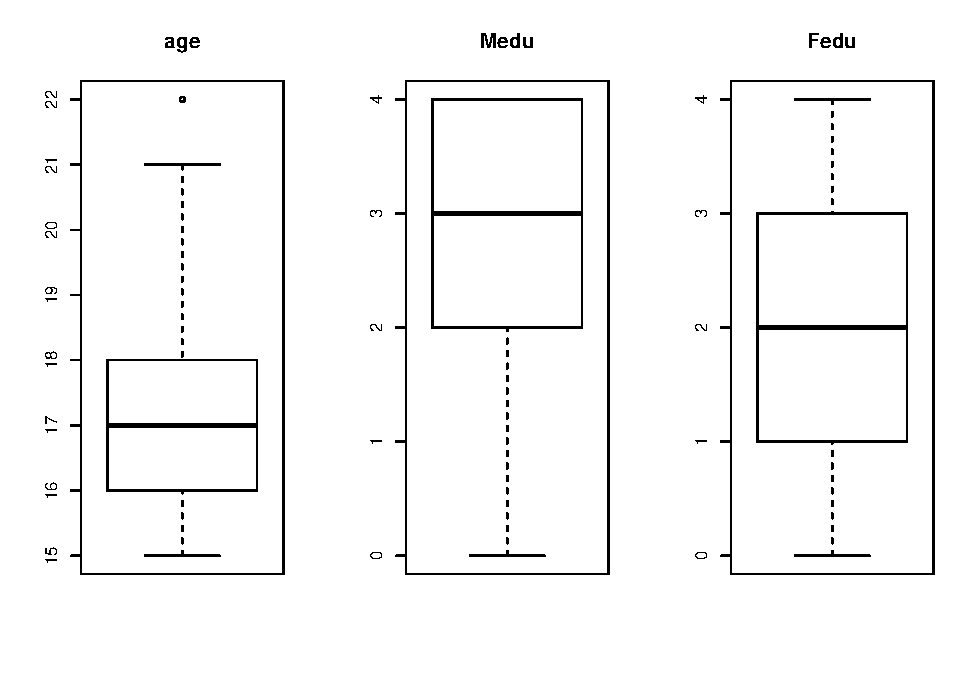
\includegraphics{Practica2_files/figure-latex/unnamed-chunk-13-1.pdf}
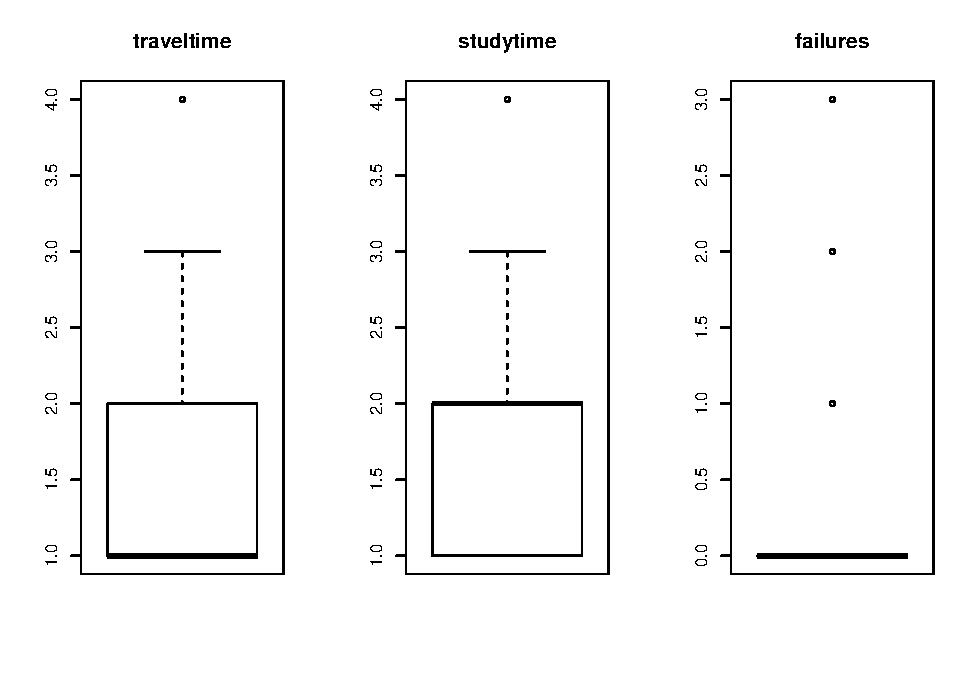
\includegraphics{Practica2_files/figure-latex/unnamed-chunk-13-2.pdf}
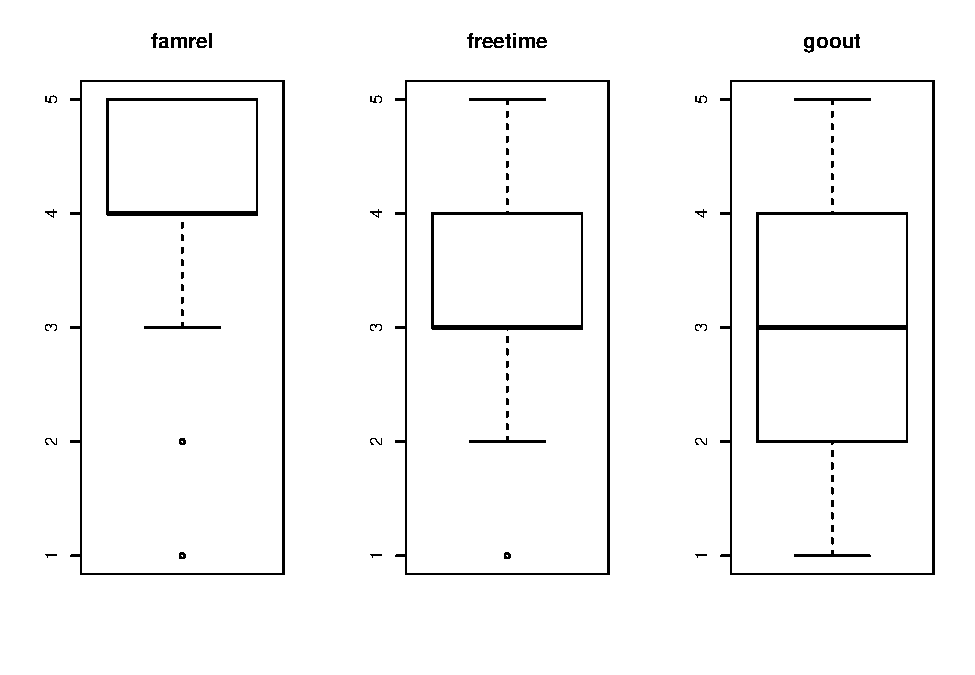
\includegraphics{Practica2_files/figure-latex/unnamed-chunk-13-3.pdf}
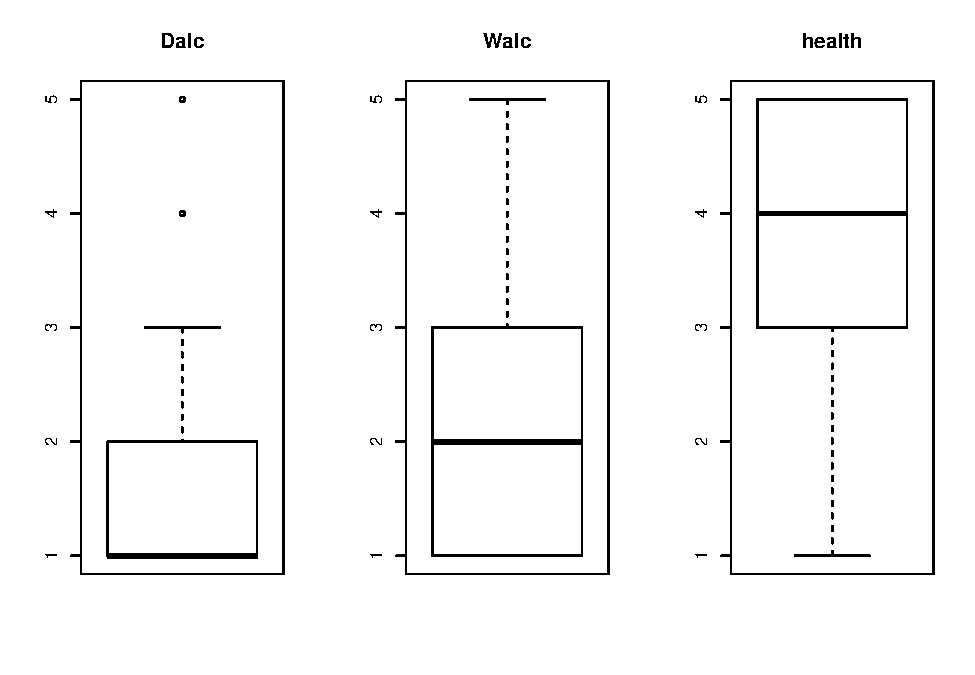
\includegraphics{Practica2_files/figure-latex/unnamed-chunk-13-4.pdf}
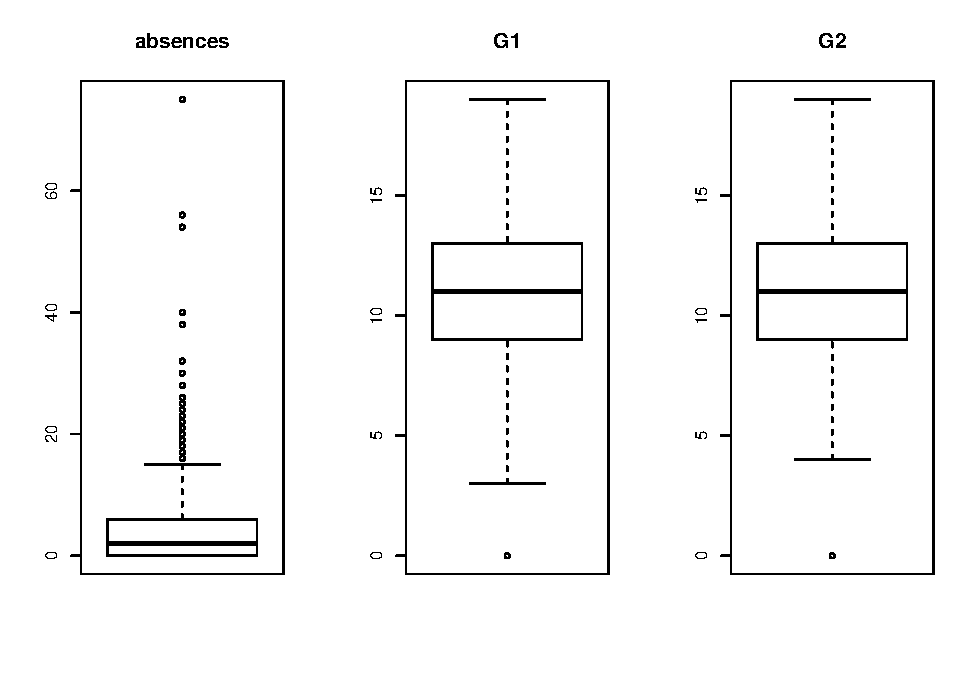
\includegraphics{Practica2_files/figure-latex/unnamed-chunk-13-5.pdf}
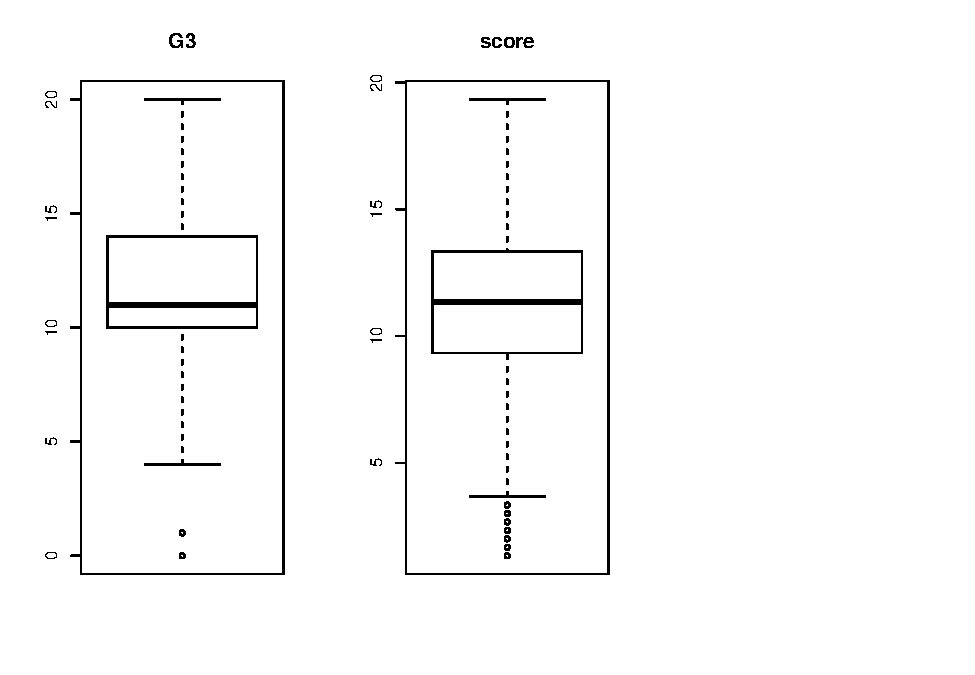
\includegraphics{Practica2_files/figure-latex/unnamed-chunk-13-6.pdf}

Vamos a analizar los diferentes outliers para cada una de las variables
numéricas:

Hemos encontrado información interesante para el tratamiento de los
outliers en la siguiente dirección web

\url{https://www.ugr.es/~fmocan/MATERIALES\%20DOCTORADO/Tratamiento\%20de\%20outliers\%20y\%20missing.pdf}

Variable Age: Vemos que hay un outlier en el valor 22. En este caso
consideramos que este valor no debería eliminarse y deberia tratarse
como uno más, probablemente el hecho de que haya alumnos de 22 años en
el mismos curso que alumnos de 18 años estará relacionado con algunas de
las variables que queremos analizar, principalmente las notas.

Variables Medu y Fedu: No tienen valores extremos.

Variable traveltime: Vemos que hay un outlier en el valor 4. Es decir,
se dan casos extremos en los que los alumnos tardan 4 horas en llegar al
colegio. Vamos a ver cuántas veces se da este valor en nuestra muestra

\begin{Shaded}
\begin{Highlighting}[]
\KeywordTok{length}\NormalTok{(}\KeywordTok{boxplot.stats}\NormalTok{(students[,}\KeywordTok{c}\NormalTok{(}\StringTok{"traveltime"}\NormalTok{)])}\OperatorTok{$}\NormalTok{out)}
\end{Highlighting}
\end{Shaded}

\begin{verbatim}
## [1] 24
\end{verbatim}

Vemos que tenemos 24 alumnos que tardan más de 3 horas en ir al colegio.
El tiempo que tardan los alumnos en llegar al colegio no es una
varaiable sobre la que queramos realizar hipótesis, como además, el
número total de outliers para este atributo es 24, esto representa el
2\% de la muestra así que los eliminamos.

\begin{Shaded}
\begin{Highlighting}[]
\NormalTok{students =}\StringTok{ }\NormalTok{students[students}\OperatorTok{$}\NormalTok{traveltime}\OperatorTok{<=}\DecValTok{3}\NormalTok{,]}
\end{Highlighting}
\end{Shaded}

La variable tiempo de estudio studytime vemos que también tiene un
outlier en el valor 4. El tiempo de estudio de los alumnos sí que
pensamos que es una variable que puede influir en los resultados finales
y es una de los atributos que vamos a tener en cuenta en nuestros
análisis. No consideramos que el 4 sea un outlier que haya ni que
eliminar ni tratar puesto que es un valor aceptable para nuestro
estudio, luego con este outlier no hacemos nada.

Lo mismo pasa con la variable que mide los suspensos, los valores que
aparecen representados como outliers son precisamente los valores que
pueden ser relevantes para nuestro estudio, luego no hacemos nada con
ellos

La variable freetime tiene un outlier en el valor 1, vamos a ver cuántos
estudiantes cumplen esta condición.

\begin{Shaded}
\begin{Highlighting}[]
\NormalTok{students[students}\OperatorTok{$}\NormalTok{freetime}\OperatorTok{==}\DecValTok{1}\NormalTok{,]}
\end{Highlighting}
\end{Shaded}

\begin{verbatim}
##      school sex age address famsize Pstatus Medu Fedu     Mjob     Fjob
## 8        GP   F  17       U     GT3       A    4    4    other  teacher
## 20       GP   M  16       U     LE3       T    4    3   health    other
## 69       GP   F  15       R     LE3       T    2    2   health services
## 90       GP   M  16       U     LE3       A    4    4  teacher   health
## 96       GP   F  15       R     GT3       T    1    1  at_home    other
## 107      GP   F  15       U     GT3       T    2    2    other    other
## 112      GP   F  16       R     GT3       T    3    3 services    other
## 113      GP   F  16       U     GT3       T    2    2  at_home    other
## 169      GP   F  16       U     GT3       T    2    2    other    other
## 190      GP   M  17       R     GT3       T    1    2  at_home    other
## 239      GP   F  17       R     GT3       T    2    1  at_home services
## 261      GP   F  18       U     GT3       T    4    3 services    other
## 277      GP   F  18       R     GT3       A    3    2    other services
## 294      GP   F  17       R     LE3       T    3    1 services    other
## 302      GP   M  17       U     LE3       T    4    4    other  teacher
## 315      GP   F  19       U     GT3       T    1    1  at_home   health
## 316      GP   F  19       R     GT3       T    2    3    other    other
## 379      MS   F  18       U     GT3       T    3    3    other    other
## 390      MS   F  18       U     GT3       T    1    1    other    other
## 403      GP   F  17       U     GT3       A    4    4    other  teacher
## 415      GP   M  16       U     LE3       T    4    3   health    other
## 464      GP   F  15       R     LE3       T    2    2   health services
## 485      GP   M  16       U     LE3       A    4    4  teacher   health
## 491      GP   F  15       R     GT3       T    1    1  at_home    other
## 502      GP   F  15       U     GT3       T    2    2    other    other
## 507      GP   F  16       R     GT3       T    3    3 services    other
## 508      GP   F  16       U     GT3       T    2    2  at_home    other
## 578      GP   F  16       U     GT3       T    2    2    other    other
## 599      GP   M  17       R     GT3       T    1    2  at_home    other
## 651      GP   F  18       U     GT3       T    3    3    other    other
## 657      GP   F  17       R     GT3       T    2    1  at_home services
## 660      GP   F  17       U     LE3       A    2    2    other    other
## 696      GP   F  18       U     GT3       T    4    3 services    other
## 714      GP   F  18       R     GT3       A    3    2    other services
## 734      GP   F  17       R     LE3       T    3    1 services    other
## 742      GP   M  17       U     LE3       T    4    4    other  teacher
## 756      GP   F  18       U     GT3       T    3    3  at_home    other
## 802      GP   F  17       U     GT3       T    3    1    other  at_home
## 814      GP   M  18       R     GT3       T    2    3    other services
## 816      GP   F  18       U     LE3       A    2    2 services    other
## 818      GP   F  18       U     GT3       T    3    2 services    other
## 821      MS   F  15       R     GT3       T    1    1  at_home services
## 835      MS   F  15       R     GT3       T    3    3    other services
## 845      MS   F  15       R     GT3       T    1    2    other services
## 887      MS   F  19       U     GT3       T    1    1    other    other
## 909      MS   F  16       U     GT3       T    3    1    other    other
## 910      MS   F  16       U     GT3       T    3    2 services  at_home
## 924      MS   F  17       R     GT3       T    2    2  at_home    other
## 925      MS   F  16       U     LE3       T    4    4 services services
## 926      MS   M  17       U     GT3       T    3    3 services services
## 927      MS   M  17       U     GT3       T    1    1  at_home services
## 930      MS   M  16       U     LE3       T    4    4  teacher   health
## 937      MS   F  17       R     GT3       T    2    2    other    other
## 940      MS   M  17       R     LE3       T    1    3    other    other
## 943      MS   M  16       R     LE3       T    4    1    other  at_home
## 946      MS   M  16       U     LE3       A    2    2    other services
## 947      MS   M  17       U     GT3       T    3    2    other    other
## 949      MS   M  17       U     LE3       A    1    0    other    other
## 994      MS   M  18       U     LE3       T    1    2  at_home services
## 1005     MS   F  18       U     GT3       T    1    2  at_home  at_home
## 1030     MS   F  18       U     GT3       T    3    3    other    other
## 1042     MS   F  18       U     GT3       T    1    1    other    other
##          reason guardian traveltime studytime failures schoolsup famsup
## 8          home   mother          2         2        0       yes    yes
## 20         home   father          1         1        0        no     no
## 69   reputation   mother          2         2        0       yes    yes
## 90   reputation   mother          1         2        0        no    yes
## 96         home   mother          2         4        1       yes    yes
## 107      course   mother          1         4        0       yes    yes
## 112  reputation   father          1         3        1       yes    yes
## 113        home   mother          1         2        1       yes     no
## 169        home   mother          1         2        0        no    yes
## 190        home   mother          1         2        0        no     no
## 239      course   mother          3         2        0        no     no
## 261        home   father          1         2        0        no    yes
## 277        home   mother          2         2        0        no     no
## 294  reputation   mother          2         4        0        no    yes
## 302        home   father          2         1        0        no     no
## 315        home    other          1         3        2        no     no
## 316  reputation    other          1         3        1        no     no
## 379        home   mother          1         2        0        no     no
## 390      course   mother          2         2        1        no     no
## 403        home   mother          2         2        0       yes    yes
## 415        home   father          1         1        0        no     no
## 464  reputation   mother          2         2        0       yes    yes
## 485  reputation   mother          1         2        0        no    yes
## 491        home   mother          2         4        0       yes    yes
## 502      course   mother          1         4        0       yes    yes
## 507  reputation   father          1         3        0       yes    yes
## 508        home   mother          1         2        1       yes     no
## 578        home   mother          1         2        0        no    yes
## 599        home   mother          1         2        0        no     no
## 651      course   mother          2         1        1        no     no
## 657      course   mother          3         2        0        no     no
## 660        home   mother          1         1        1        no    yes
## 696        home   father          1         2        0        no    yes
## 714        home   mother          2         2        0        no     no
## 734  reputation   mother          2         4        0        no    yes
## 742        home   father          2         1        0        no     no
## 756      course   father          1         2        0        no    yes
## 802        home   mother          1         1        1        no    yes
## 814  reputation   father          1         1        0        no     no
## 816  reputation   mother          2         2        0        no    yes
## 818        home   mother          1         2        0        no    yes
## 821       other   mother          1         1        1        no    yes
## 835      course   father          2         1        0        no     no
## 845      course   mother          2         1        0        no     no
## 887      course    other          2         2        1        no    yes
## 909      course   mother          1         1        0        no     no
## 910      course   mother          1         1        0        no     no
## 924       other   mother          1         1        0        no    yes
## 925       other   father          2         1        0        no    yes
## 926        home   mother          1         1        0        no    yes
## 927       other   mother          3         2        0        no     no
## 930       other   father          1         1        0        no    yes
## 937       other   mother          2         2        0       yes     no
## 940      course   father          2         1        0        no     no
## 943       other   father          1         1        0        no     no
## 946      course   father          2         2        0        no    yes
## 947       other   father          2         2        0        no    yes
## 949        home   mother          1         1        0        no     no
## 994        home   mother          2         1        0        no    yes
## 1005     course   father          2         2        0        no    yes
## 1030       home   mother          1         2        0        no     no
## 1042     course   mother          2         2        0        no     no
##      paid activities nursery higher internet romantic famrel freetime
## 8      no         no     yes    yes       no       no      4        1
## 20    yes        yes     yes    yes      yes       no      3        1
## 69    yes         no     yes    yes      yes       no      4        1
## 90     no         no     yes    yes       no       no      4        1
## 96    yes        yes     yes    yes      yes       no      3        1
## 107   yes         no     yes    yes      yes       no      5        1
## 112    no        yes     yes    yes      yes       no      4        1
## 113    no        yes     yes    yes      yes       no      3        1
## 169   yes         no      no    yes      yes       no      5        1
## 190    no         no     yes    yes       no       no      3        1
## 239    no        yes     yes    yes       no       no      2        1
## 261   yes         no     yes    yes      yes      yes      3        1
## 277    no         no      no     no      yes      yes      4        1
## 294   yes         no     yes    yes       no       no      3        1
## 302   yes         no     yes    yes      yes       no      4        1
## 315    no         no      no    yes      yes      yes      4        1
## 316    no         no     yes    yes      yes      yes      4        1
## 379   yes         no     yes    yes      yes      yes      4        1
## 390    no        yes     yes    yes       no       no      1        1
## 403    no         no     yes    yes       no       no      4        1
## 415    no        yes     yes    yes      yes       no      3        1
## 464    no         no     yes    yes      yes       no      4        1
## 485    no         no     yes    yes       no       no      4        1
## 491   yes        yes     yes    yes      yes       no      3        1
## 502    no         no     yes    yes      yes       no      5        1
## 507    no        yes     yes    yes      yes       no      4        1
## 508    no        yes     yes    yes      yes       no      3        1
## 578    no         no      no    yes      yes       no      5        1
## 599    no         no     yes    yes       no       no      3        1
## 651    no         no     yes     no      yes       no      4        1
## 657    no        yes     yes    yes       no       no      2        1
## 660    no         no      no     no      yes       no      3        1
## 696    no         no     yes    yes      yes      yes      3        1
## 714    no         no      no     no      yes      yes      4        1
## 734    no         no     yes    yes       no       no      3        1
## 742    no         no     yes    yes      yes       no      4        1
## 756    no         no     yes    yes      yes       no      4        1
## 802   yes         no     yes    yes      yes      yes      4        1
## 814    no         no     yes    yes      yes       no      3        1
## 816    no         no     yes    yes      yes       no      4        1
## 818    no        yes      no    yes      yes      yes      3        1
## 821    no         no     yes    yes       no      yes      4        1
## 835    no         no      no    yes      yes       no      4        1
## 845    no         no     yes    yes       no       no      5        1
## 887    no         no     yes    yes      yes      yes      1        1
## 909    no        yes     yes    yes      yes       no      3        1
## 910    no         no     yes    yes      yes       no      3        1
## 924   yes         no     yes    yes      yes       no      5        1
## 925    no         no     yes    yes       no       no      5        1
## 926    no        yes     yes    yes      yes       no      4        1
## 927    no         no     yes    yes      yes      yes      5        1
## 930    no         no     yes    yes      yes       no      4        1
## 937   yes         no     yes    yes       no       no      5        1
## 940    no        yes     yes    yes       no      yes      5        1
## 943    no         no     yes    yes      yes       no      4        1
## 946    no         no      no    yes      yes      yes      4        1
## 947   yes         no     yes    yes      yes       no      4        1
## 949    no         no     yes    yes       no      yes      4        1
## 994    no         no      no    yes       no       no      4        1
## 1005   no         no     yes     no       no       no      4        1
## 1030   no         no     yes    yes      yes      yes      4        1
## 1042   no        yes     yes    yes       no       no      1        1
##      goout Dalc Walc health absences G1 G2 G3  id     score mark
## 8        4    1    1      1        6  6  5  6 121  5.666667 fail
## 20       3    1    3      5        4  8 10 10 340  9.333333 fail
## 69       3    1    3      4        2  8  9  8   9  8.333333 fail
## 90       3    3    5      5       18  8  6  7 329  7.000000 fail
## 96       2    1    1      1        2  7 10 10   1  9.000000 fail
## 107      2    1    1      3        8  7  8  8  21  7.666667 fail
## 112      2    1    1      2        0  7 10 10  46  9.000000 fail
## 113      2    1    1      5        6 10 13 13  61 12.000000 pass
## 169      5    1    1      4        0  6  7  0  62  4.333333 fail
## 190      3    1    5      3        4  8  9 10 345  9.000000 fail
## 239      1    1    1      3        2 13 11 11 103 11.666667 pass
## 261      2    1    3      2       21 17 18 18 208 17.666667 pass
## 277      1    1    1      5       75 10  9  9 175  9.333333 fail
## 294      2    1    1      3        6 18 18 18 115 18.000000 pass
## 302      1    2    2      5        0 11 11 10 383 10.666667 pass
## 315      2    1    1      3       14 15 13 13 228 13.666667 pass
## 316      2    1    1      3       40 13 11 11 225 11.666667 pass
## 379      3    1    2      1        0 15 15 15 558 15.000000 pass
## 390      1    1    1      5        0  6  5  0 552  3.666667 fail
## 403      4    1    1      1        2 10 13 13 121 12.000000 pass
## 415      3    1    3      5        6 12 12 12 340 12.000000 pass
## 464      3    1    3      4        0 11 10 11   9 10.666667 pass
## 485      3    3    5      5        6  9  9 10 329  9.333333 fail
## 491      2    1    1      1        4 13 13 13   1 13.000000 pass
## 502      2    1    1      3        4 10 10 10  21 10.000000 pass
## 507      2    1    1      2        4 11 11 11  46 11.000000 pass
## 508      2    1    1      5       12  8 10 10  61  9.333333 fail
## 578      5    1    1      4        0 12 12 13  62 12.333333 pass
## 599      3    1    5      3        6  9  9 10 345  9.333333 fail
## 651      1    1    1      3       14  8  7  7 203  7.333333 fail
## 657      1    1    1      3        2 13 13 13 103 13.000000 pass
## 660      2    1    1      1        8 11  9 10 161 10.000000 pass
## 696      2    1    3      2        2 15 15 15 208 15.000000 pass
## 714      1    1    1      5       15 12  9 10 175 10.333333 pass
## 734      2    1    1      3        0 18 19 19 115 18.666667 pass
## 742      1    2    2      5        0 12 13 13 383 12.666667 pass
## 756      4    1    1      3        8 11 12 14 202 12.333333 pass
## 802      2    1    1      3        6 10 13 13 140 12.000000 pass
## 814      3    4    5      4       13 13 14 14 387 13.666667 pass
## 816      4    1    3      4       10 14 17 17 212 16.000000 pass
## 818      2    1    2      1        4 10 13 13 201 12.000000 pass
## 821      3    1    1      2        6 10 10 10 437 10.000000 pass
## 835      3    1    1      4        0 14 16 16 440 15.333333 pass
## 845      2    1    1      1        3 11 13 13 438 12.333333 pass
## 887      4    4    1      1       12  7  8  9 573  8.000000 fail
## 909      3    1    3      1        0  8  6  8 482  7.333333 fail
## 910      3    1    4      3        2  7  6  7 483  6.666667 fail
## 924      3    1    2      5        5  9  9  9 502  9.000000 fail
## 925      3    1    2      5        1 11 11 11 492 11.000000 pass
## 926      4    5    5      3        8  7 10  9 627  8.666667 fail
## 927      3    3    3      1        0 10 10 10 619 10.000000 pass
## 930      2    2    5      5        0 11 12 12 608 11.666667 pass
## 937      3    1    1      5        0 11  9 11 503 10.333333 pass
## 940      2    3    3      5        2 12 11 12 617 11.666667 pass
## 943      2    2    1      2        0 10 11 11 599 10.666667 pass
## 946      2    2    2      5        0 12 13 13 604 12.666667 pass
## 947      2    2    2      1        0 13 14 13 624 13.333333 pass
## 949      2    1    1      5        4 11 11 12 629 11.333333 pass
## 994      4    5    5      1        8 10 11 11 648 10.666667 pass
## 1005     1    1    1      4        0 11 11 12 553 11.333333 pass
## 1030     3    1    2      1        1 16 16 16 558 16.000000 pass
## 1042     1    1    1      5        6 11 12  9 552 10.666667 pass
##      calification    subject
## 8               F       Math
## 20              F       Math
## 69              F       Math
## 90              F       Math
## 96              F       Math
## 107             F       Math
## 112             F       Math
## 113             C       Math
## 169             F       Math
## 190             F       Math
## 239             D       Math
## 261             A       Math
## 277             F       Math
## 294             A       Math
## 302             D       Math
## 315             C       Math
## 316             D       Math
## 379             B       Math
## 390             F       Math
## 403             C Portuguese
## 415             C Portuguese
## 464             D Portuguese
## 485             F Portuguese
## 491             C Portuguese
## 502             D Portuguese
## 507             D Portuguese
## 508             F Portuguese
## 578             C Portuguese
## 599             F Portuguese
## 651             F Portuguese
## 657             C Portuguese
## 660             D Portuguese
## 696             B Portuguese
## 714             D Portuguese
## 734             A Portuguese
## 742             C Portuguese
## 756             C Portuguese
## 802             C Portuguese
## 814             C Portuguese
## 816             A Portuguese
## 818             C Portuguese
## 821             D Portuguese
## 835             B Portuguese
## 845             C Portuguese
## 887             F Portuguese
## 909             F Portuguese
## 910             F Portuguese
## 924             F Portuguese
## 925             D Portuguese
## 926             F Portuguese
## 927             D Portuguese
## 930             D Portuguese
## 937             D Portuguese
## 940             D Portuguese
## 943             D Portuguese
## 946             C Portuguese
## 947             C Portuguese
## 949             D Portuguese
## 994             D Portuguese
## 1005            D Portuguese
## 1030            A Portuguese
## 1042            D Portuguese
\end{verbatim}

Son 64 alumnos que tienen muy poco tiempo libre entre semana. Puesto que
este valor está relacionado con el tiempo de estudio semanal y con las
ayudas extrasescolares que puedan recibir los alumnos decidimos
mantenerlos también.

Variable famrel: Tenemos outliers en 1 y 2. Estos valores miden la
calidad de las relaciones familiares, entendiendo que estos valores se
han obtenido a través de una encuesta a los propios alumnos. El valor de
1 es tan bajo que pensamos que puede deberse a una manipulación por
parte de los alumnos en las respuestas. Consideramos que una forma de
tratar estos outliers es reemplazarlos por la moda (más repetida). Los
valores de 2 los dejaremos como están puesto que no nos parece que
puedan considrarse como outliers. Para calcular la moda utilizamos una
tabla de frecuencia para contar el número de veces que se repite cada
valor:

\begin{Shaded}
\begin{Highlighting}[]
\KeywordTok{table}\NormalTok{(students}\OperatorTok{$}\NormalTok{famrel)}
\end{Highlighting}
\end{Shaded}

\begin{verbatim}
## 
##   1   2   3   4   5 
##  28  47 168 501 276
\end{verbatim}

Vemos que el valor más repetido es el 4, luego sustituimos aquellas
columnas que tengan el valor 1 en la columna famrel por 4

\begin{Shaded}
\begin{Highlighting}[]
\NormalTok{students}\OperatorTok{$}\NormalTok{famrel[students}\OperatorTok{$}\NormalTok{famrel }\OperatorTok{==}\StringTok{ }\DecValTok{1}\NormalTok{] <-}\StringTok{ }\DecValTok{4}
\end{Highlighting}
\end{Shaded}

En el caso del consumo diario de alcohol, tenemos un outlier en los
valores 4 y 5. Sin embargo no tenemos estos outliers en el consumo del
fin de semana. Pensamos por tanto que el hecho de que alumnos consuman
mucho alcohol durante los días de diario puede estar relacionado con las
notas que obtengan, así que vamos a dejar estos valores.

\begin{Shaded}
\begin{Highlighting}[]
\KeywordTok{length}\NormalTok{(}\KeywordTok{boxplot.stats}\NormalTok{(students[,}\KeywordTok{c}\NormalTok{(}\StringTok{"Dalc"}\NormalTok{)])}\OperatorTok{$}\NormalTok{out)}
\end{Highlighting}
\end{Shaded}

\begin{verbatim}
## [1] 46
\end{verbatim}

Para el caso de las ausencias, nos interesa saber cuántos outliers
tenemos y qué valores toman para poder analizar cómo tratarlos.

\begin{Shaded}
\begin{Highlighting}[]
\KeywordTok{length}\NormalTok{(}\KeywordTok{boxplot.stats}\NormalTok{(students[,}\KeywordTok{c}\NormalTok{(}\StringTok{"absences"}\NormalTok{)])}\OperatorTok{$}\NormalTok{out)}
\end{Highlighting}
\end{Shaded}

\begin{verbatim}
## [1] 54
\end{verbatim}

\begin{Shaded}
\begin{Highlighting}[]
\KeywordTok{boxplot.stats}\NormalTok{(students[,}\KeywordTok{c}\NormalTok{(}\StringTok{"absences"}\NormalTok{)])}\OperatorTok{$}\NormalTok{out}
\end{Highlighting}
\end{Shaded}

\begin{verbatim}
##  [1] 16 16 25 54 18 26 20 18 16 16 56 24 18 28 22 16 18 20 16 21 75 22 30
## [24] 19 20 38 18 20 22 40 23 16 17 16 16 24 22 16 32 16 16 30 21 16 18 16
## [47] 26 16 16 22 18 18 16 21
\end{verbatim}

\begin{Shaded}
\begin{Highlighting}[]
\NormalTok{students[students}\OperatorTok{$}\NormalTok{absences}\OperatorTok{>=}\DecValTok{40}\NormalTok{,]}
\end{Highlighting}
\end{Shaded}

\begin{verbatim}
##     school sex age address famsize Pstatus Medu Fedu  Mjob     Fjob
## 75      GP   F  16       U     GT3       T    3    3 other services
## 184     GP   F  17       U     LE3       T    3    3 other    other
## 277     GP   F  18       R     GT3       A    3    2 other services
## 316     GP   F  19       R     GT3       T    2    3 other    other
##         reason guardian traveltime studytime failures schoolsup famsup
## 75        home   mother          1         2        0       yes    yes
## 184 reputation   mother          1         2        0        no    yes
## 277       home   mother          2         2        0        no     no
## 316 reputation    other          1         3        1        no     no
##     paid activities nursery higher internet romantic famrel freetime goout
## 75   yes        yes     yes    yes      yes       no      4        3     3
## 184   no        yes     yes    yes      yes      yes      5        3     3
## 277   no         no      no     no      yes      yes      4        1     1
## 316   no         no     yes    yes      yes      yes      4        1     2
##     Dalc Walc health absences G1 G2 G3  id     score mark calification
## 75     2    4      5       54 11 12 11  75 11.333333 pass            D
## 184    2    3      1       56  9  9  8 172  8.666667 fail            F
## 277    1    1      5       75 10  9  9 175  9.333333 fail            F
## 316    1    1      3       40 13 11 11 225 11.666667 pass            D
##     subject
## 75     Math
## 184    Math
## 277    Math
## 316    Math
\end{verbatim}

A la vista de los resultados vemos que tenemos 54 outliers en las
ausencias, y que los valores que toman en estos outliers son 16 16 25 54
18 26 20 18 16 16 56 24 18 28 22 16 18 20 16 21 75 22 30 19 20 38 18 20
22 40 23 16 17 16 16 24 22 16 32 Nos parece que los valores que están en
un intervalo de (10,30) son admisibles, sin embargo, vemos que hay
valores que pasan de 40 que podrían eliminarse.

En total, vamos a contar cuántos datos tenemos para ausencias mayores o
iguales que 40

\begin{Shaded}
\begin{Highlighting}[]
\NormalTok{students[students}\OperatorTok{$}\NormalTok{absences}\OperatorTok{>=}\DecValTok{40}\NormalTok{,]}
\end{Highlighting}
\end{Shaded}

\begin{verbatim}
##     school sex age address famsize Pstatus Medu Fedu  Mjob     Fjob
## 75      GP   F  16       U     GT3       T    3    3 other services
## 184     GP   F  17       U     LE3       T    3    3 other    other
## 277     GP   F  18       R     GT3       A    3    2 other services
## 316     GP   F  19       R     GT3       T    2    3 other    other
##         reason guardian traveltime studytime failures schoolsup famsup
## 75        home   mother          1         2        0       yes    yes
## 184 reputation   mother          1         2        0        no    yes
## 277       home   mother          2         2        0        no     no
## 316 reputation    other          1         3        1        no     no
##     paid activities nursery higher internet romantic famrel freetime goout
## 75   yes        yes     yes    yes      yes       no      4        3     3
## 184   no        yes     yes    yes      yes      yes      5        3     3
## 277   no         no      no     no      yes      yes      4        1     1
## 316   no         no     yes    yes      yes      yes      4        1     2
##     Dalc Walc health absences G1 G2 G3  id     score mark calification
## 75     2    4      5       54 11 12 11  75 11.333333 pass            D
## 184    2    3      1       56  9  9  8 172  8.666667 fail            F
## 277    1    1      5       75 10  9  9 175  9.333333 fail            F
## 316    1    1      3       40 13 11 11 225 11.666667 pass            D
##     subject
## 75     Math
## 184    Math
## 277    Math
## 316    Math
\end{verbatim}

Vemos que tenemos 4 valores, luego decidimos eliminarlos de nuestro
objeto de estudio

\begin{Shaded}
\begin{Highlighting}[]
\NormalTok{students =}\StringTok{ }\NormalTok{students[students}\OperatorTok{$}\NormalTok{absences}\OperatorTok{<}\DecValTok{40}\NormalTok{,]}
\KeywordTok{glimpse}\NormalTok{(students)}
\end{Highlighting}
\end{Shaded}

\begin{verbatim}
## Observations: 1,016
## Variables: 38
## $ school       <fct> GP, GP, GP, GP, GP, GP, GP, GP, GP, GP, GP, GP, G...
## $ sex          <fct> F, F, F, F, F, M, M, F, M, M, F, F, M, M, M, F, F...
## $ age          <int> 18, 17, 15, 15, 16, 16, 16, 17, 15, 15, 15, 15, 1...
## $ address      <fct> U, U, U, U, U, U, U, U, U, U, U, U, U, U, U, U, U...
## $ famsize      <fct> GT3, GT3, LE3, GT3, GT3, LE3, LE3, GT3, LE3, GT3,...
## $ Pstatus      <fct> A, T, T, T, T, T, T, A, A, T, T, T, T, T, A, T, T...
## $ Medu         <int> 4, 1, 1, 4, 3, 4, 2, 4, 3, 3, 4, 2, 4, 4, 2, 4, 4...
## $ Fedu         <int> 4, 1, 1, 2, 3, 3, 2, 4, 2, 4, 4, 1, 4, 3, 2, 4, 4...
## $ Mjob         <fct> at_home, at_home, at_home, health, other, service...
## $ Fjob         <fct> teacher, other, other, services, other, other, ot...
## $ reason       <fct> course, course, other, home, home, reputation, ho...
## $ guardian     <fct> mother, father, mother, mother, father, mother, m...
## $ traveltime   <int> 2, 1, 1, 1, 1, 1, 1, 2, 1, 1, 1, 3, 1, 2, 1, 1, 1...
## $ studytime    <int> 2, 2, 2, 3, 2, 2, 2, 2, 2, 2, 2, 3, 1, 2, 3, 1, 3...
## $ failures     <int> 0, 0, 3, 0, 0, 0, 0, 0, 0, 0, 0, 0, 0, 0, 0, 0, 0...
## $ schoolsup    <fct> yes, no, yes, no, no, no, no, yes, no, no, no, no...
## $ famsup       <fct> no, yes, no, yes, yes, yes, no, yes, yes, yes, ye...
## $ paid         <fct> no, no, yes, yes, yes, yes, no, no, yes, yes, yes...
## $ activities   <fct> no, no, no, yes, no, yes, no, no, no, yes, no, ye...
## $ nursery      <fct> yes, no, yes, yes, yes, yes, yes, yes, yes, yes, ...
## $ higher       <fct> yes, yes, yes, yes, yes, yes, yes, yes, yes, yes,...
## $ internet     <fct> no, yes, yes, yes, no, yes, yes, no, yes, yes, ye...
## $ romantic     <fct> no, no, no, yes, no, no, no, no, no, no, no, no, ...
## $ famrel       <dbl> 4, 5, 4, 3, 4, 5, 4, 4, 4, 5, 3, 5, 4, 5, 4, 4, 3...
## $ freetime     <int> 3, 3, 3, 2, 3, 4, 4, 1, 2, 5, 3, 2, 3, 4, 5, 4, 2...
## $ goout        <int> 4, 3, 2, 2, 2, 2, 4, 4, 2, 1, 3, 2, 3, 3, 2, 4, 3...
## $ Dalc         <int> 1, 1, 2, 1, 1, 1, 1, 1, 1, 1, 1, 1, 1, 1, 1, 1, 1...
## $ Walc         <int> 1, 1, 3, 1, 2, 2, 1, 1, 1, 1, 2, 1, 3, 2, 1, 2, 2...
## $ health       <int> 3, 3, 3, 5, 5, 5, 3, 1, 1, 5, 2, 4, 5, 3, 3, 2, 2...
## $ absences     <int> 6, 4, 10, 2, 4, 10, 0, 6, 0, 0, 0, 4, 2, 2, 0, 4,...
## $ G1           <int> 5, 5, 7, 15, 6, 15, 12, 6, 16, 14, 10, 10, 14, 10...
## $ G2           <int> 6, 5, 8, 14, 10, 15, 12, 5, 18, 15, 8, 12, 14, 10...
## $ G3           <int> 6, 6, 10, 15, 10, 15, 11, 6, 19, 15, 9, 12, 14, 1...
## $ id           <fct> 184, 123, 39, 25, 72, 341, 336, 121, 279, 260, 32...
## $ score        <dbl> 5.666667, 5.333333, 8.333333, 14.666667, 8.666667...
## $ mark         <fct> fail, fail, fail, pass, fail, pass, pass, fail, p...
## $ calification <fct> F, F, F, B, F, B, D, F, A, B, F, D, B, D, B, B, C...
## $ subject      <fct> Math, Math, Math, Math, Math, Math, Math, Math, M...
\end{verbatim}

Las columnas relativas a las notas van a ser principalmente las que sean
objeto de estudio. Tenemos outliers en notas que son perfectamente
posibles, luego no vamos a eliminarlo puesto que pensamos que estos
valores afectarán a los estudios e hipótesis que queramos estudiar.

\hypertarget{analisis-de-los-datos}{%
\subsection{Análisis de los datos}\label{analisis-de-los-datos}}

\hypertarget{seleccion-de-los-grupos-de-datos-que-se-quieren-analizarcomparar-planificacion-de-los-analisis-a-aplicar.}{%
\subsubsection{Selección de los grupos de datos que se quieren
analizar/comparar (planificación de los análisis a
aplicar).}\label{seleccion-de-los-grupos-de-datos-que-se-quieren-analizarcomparar-planificacion-de-los-analisis-a-aplicar.}}

A continuación, se seleccionan los grupos dentro de nuestro conjunto de
datos que pueden resultar interesantes para analizar y/o comparar. No
obstante, como se verá en el apartado consistente en la realización de
pruebas estadísticas, no todos se utilizarán.

\begin{Shaded}
\begin{Highlighting}[]
\CommentTok{# school, sex, age, address, famsize, Pstatus, Medu, Fedu, Mjob, Fjob, reason, nursery, internet}
\CommentTok{# traveltime, studytime, failures, schoolsup, famsup, paid, activities, higher, romantic, famrel}
\CommentTok{# freetime, goout, Dalc, Walc, health, absences, subject}

\CommentTok{# Agrupación por sexo de los estudiantes}
\NormalTok{students.male <-}\StringTok{ }\NormalTok{students[students}\OperatorTok{$}\NormalTok{sex }\OperatorTok{==}\StringTok{ "M"}\NormalTok{,]}
\NormalTok{students.female <-}\StringTok{ }\NormalTok{students[students}\OperatorTok{$}\NormalTok{sex }\OperatorTok{==}\StringTok{ "F"}\NormalTok{,]}

\CommentTok{# Agrupación por si reciben clases particules pagadas o no}
\NormalTok{students.paid <-}\StringTok{ }\NormalTok{students[students}\OperatorTok{$}\NormalTok{paid }\OperatorTok{==}\StringTok{ "yes"}\NormalTok{,]}
\NormalTok{students.nopaid <-}\StringTok{ }\NormalTok{students[students}\OperatorTok{$}\NormalTok{paid }\OperatorTok{==}\StringTok{ "no"}\NormalTok{,]}

\CommentTok{# Agrupación por si reciben soporte por parte de la familia}
\NormalTok{students.famsup <-}\StringTok{ }\NormalTok{students[students}\OperatorTok{$}\NormalTok{famsup }\OperatorTok{==}\StringTok{ "yes"}\NormalTok{,]}
\NormalTok{students.nofamsup <-}\StringTok{ }\NormalTok{students[students}\OperatorTok{$}\NormalTok{famsup }\OperatorTok{==}\StringTok{ "no"}\NormalTok{,]}

\CommentTok{# Agrupación por si reciben ayuda extra escolar}
\NormalTok{students.schoolsup <-}\StringTok{ }\NormalTok{students[students}\OperatorTok{$}\NormalTok{schoolsup }\OperatorTok{==}\StringTok{ "yes"}\NormalTok{,]}
\NormalTok{students.noschoolsup <-}\StringTok{ }\NormalTok{students[students}\OperatorTok{$}\NormalTok{schoolsup }\OperatorTok{==}\StringTok{ "no"}\NormalTok{,]}

\CommentTok{# Agrupación por estudios de los padres}
\NormalTok{students.parentedu <-}\StringTok{ }\NormalTok{students[(students}\OperatorTok{$}\NormalTok{Medu }\OperatorTok{==}\StringTok{ "yes"}\NormalTok{) }\OperatorTok{|}\StringTok{ }\NormalTok{(students}\OperatorTok{$}\NormalTok{Medu }\OperatorTok{==}\StringTok{ "yes"}\NormalTok{),]}
\NormalTok{students.parentnoedu <-}\StringTok{ }\NormalTok{students[(students}\OperatorTok{$}\NormalTok{Medu }\OperatorTok{==}\StringTok{ "no"}\NormalTok{) }\OperatorTok{&}\StringTok{ }\NormalTok{(students}\OperatorTok{$}\NormalTok{Medu }\OperatorTok{==}\StringTok{ "no"}\NormalTok{),]}

\CommentTok{# Agrupación por tiempo dedicado al estudio}
\NormalTok{students.studytime <-}\StringTok{ }\NormalTok{students[students}\OperatorTok{$}\NormalTok{studytime }\OperatorTok{>=}\StringTok{ }\DecValTok{3}\NormalTok{,]}
\NormalTok{students.nostudytime <-}\StringTok{ }\NormalTok{students[students}\OperatorTok{$}\NormalTok{studytime }\OperatorTok{<}\StringTok{ }\DecValTok{3}\NormalTok{,]}

\CommentTok{# Agrupación por edad}
\NormalTok{students.mayores <-}\StringTok{ }\NormalTok{students[students}\OperatorTok{$}\NormalTok{age }\OperatorTok{>=}\StringTok{ }\DecValTok{16}\NormalTok{,]}
\NormalTok{students.menores <-}\StringTok{ }\NormalTok{students[students}\OperatorTok{$}\NormalTok{age }\OperatorTok{<}\StringTok{ }\DecValTok{16}\NormalTok{,]}

\CommentTok{# Agrupación por asignatura}
\NormalTok{students.port <-}\StringTok{ }\NormalTok{students[students}\OperatorTok{$}\NormalTok{port }\OperatorTok{==}\StringTok{ "yes"}\NormalTok{,]}
\NormalTok{students.math <-}\StringTok{ }\NormalTok{students[students}\OperatorTok{$}\NormalTok{math }\OperatorTok{==}\StringTok{ "yes"}\NormalTok{,]}
\end{Highlighting}
\end{Shaded}

\hypertarget{analisis-visual}{%
\subsubsection{Análisis visual}\label{analisis-visual}}

\begin{Shaded}
\begin{Highlighting}[]
\KeywordTok{ggplot}\NormalTok{(students,}\KeywordTok{aes}\NormalTok{(}\DataTypeTok{x=}\NormalTok{studytime,}\DataTypeTok{fill=}\NormalTok{calification))}\OperatorTok{+}\KeywordTok{geom_bar}\NormalTok{(}\DataTypeTok{position=}\StringTok{"fill"}\NormalTok{)}\OperatorTok{+}\KeywordTok{ylab}\NormalTok{(}\StringTok{"Porcentaje"}\NormalTok{)}\OperatorTok{+}\KeywordTok{facet_wrap}\NormalTok{(}\OperatorTok{~}\NormalTok{sex )}
\end{Highlighting}
\end{Shaded}

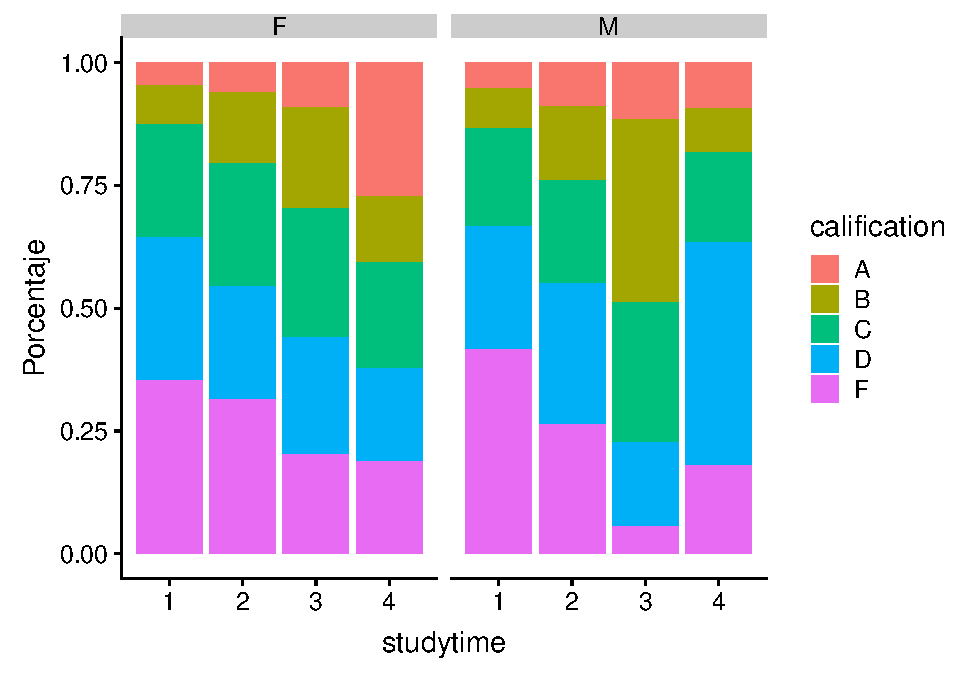
\includegraphics{Practica2_files/figure-latex/unnamed-chunk-24-1.pdf}

\begin{Shaded}
\begin{Highlighting}[]
\KeywordTok{ggplot}\NormalTok{(students,}\KeywordTok{aes}\NormalTok{(}\DataTypeTok{x=}\NormalTok{studytime,}\DataTypeTok{fill=}\NormalTok{calification))}\OperatorTok{+}\KeywordTok{geom_bar}\NormalTok{()}\OperatorTok{+}\KeywordTok{ylab}\NormalTok{(}\StringTok{"Frecuencia"}\NormalTok{)}\OperatorTok{+}\KeywordTok{facet_wrap}\NormalTok{(}\OperatorTok{~}\NormalTok{sex )}
\end{Highlighting}
\end{Shaded}

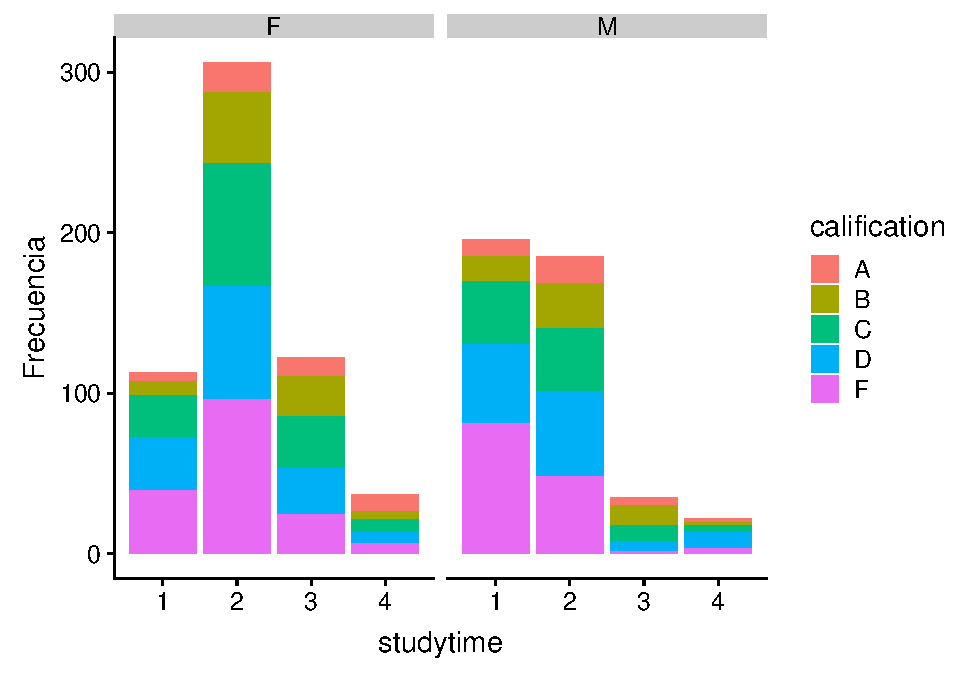
\includegraphics{Practica2_files/figure-latex/unnamed-chunk-24-2.pdf}

\begin{Shaded}
\begin{Highlighting}[]
\KeywordTok{ggplot}\NormalTok{(students,}\KeywordTok{aes}\NormalTok{(}\DataTypeTok{x=}\NormalTok{schoolsup,}\DataTypeTok{fill=}\NormalTok{calification))}\OperatorTok{+}\KeywordTok{geom_bar}\NormalTok{(}\DataTypeTok{position=}\StringTok{"fill"}\NormalTok{)}\OperatorTok{+}\KeywordTok{ylab}\NormalTok{(}\StringTok{"Porcentaje"}\NormalTok{)}\OperatorTok{+}\KeywordTok{facet_wrap}\NormalTok{(}\OperatorTok{~}\NormalTok{sex )}
\end{Highlighting}
\end{Shaded}

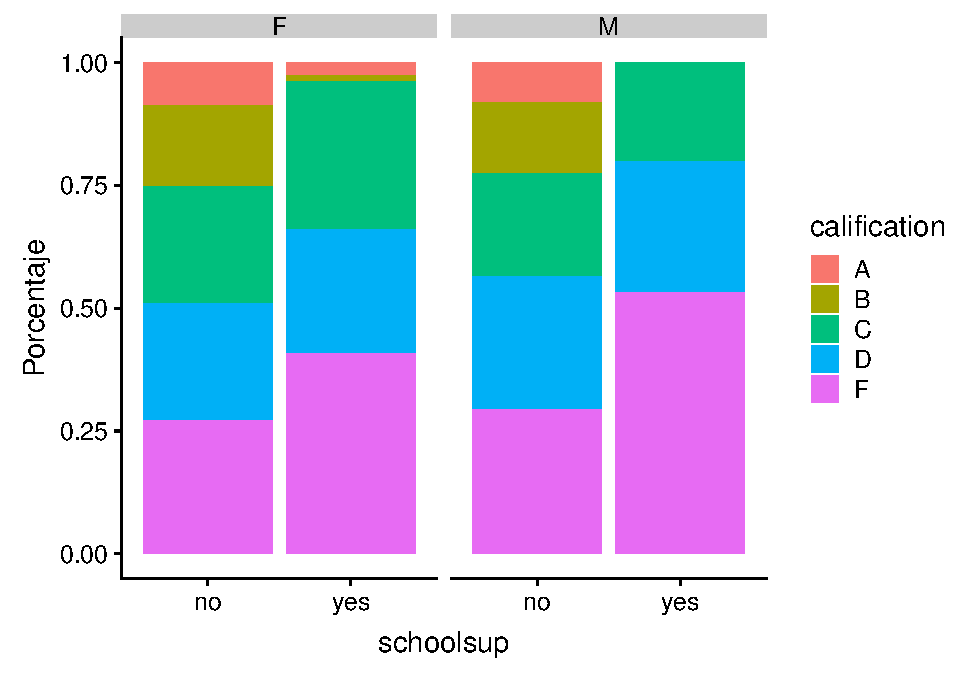
\includegraphics{Practica2_files/figure-latex/unnamed-chunk-25-1.pdf}

\begin{Shaded}
\begin{Highlighting}[]
\KeywordTok{ggplot}\NormalTok{(students,}\KeywordTok{aes}\NormalTok{(}\DataTypeTok{x=}\NormalTok{schoolsup,}\DataTypeTok{fill=}\NormalTok{calification))}\OperatorTok{+}\KeywordTok{geom_bar}\NormalTok{()}\OperatorTok{+}\KeywordTok{ylab}\NormalTok{(}\StringTok{"Frecuencia"}\NormalTok{)}\OperatorTok{+}\KeywordTok{facet_wrap}\NormalTok{(}\OperatorTok{~}\NormalTok{sex )}
\end{Highlighting}
\end{Shaded}

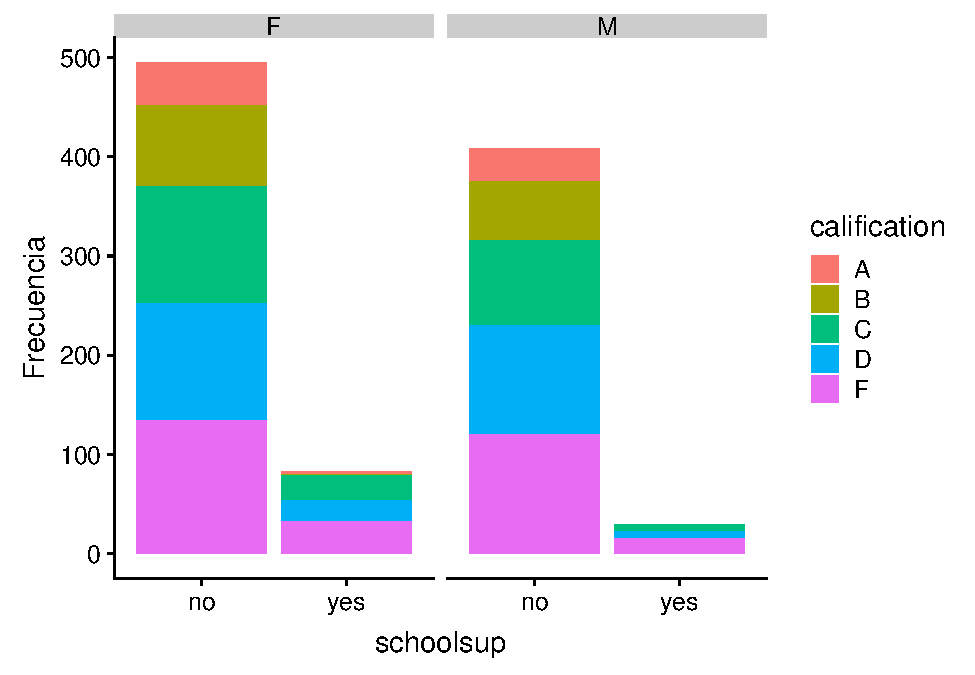
\includegraphics{Practica2_files/figure-latex/unnamed-chunk-25-2.pdf}

\begin{Shaded}
\begin{Highlighting}[]
\KeywordTok{ggplot}\NormalTok{(students,}\KeywordTok{aes}\NormalTok{(}\DataTypeTok{x=}\NormalTok{paid,}\DataTypeTok{fill=}\NormalTok{calification))}\OperatorTok{+}\KeywordTok{geom_bar}\NormalTok{(}\DataTypeTok{position=}\StringTok{"fill"}\NormalTok{)}\OperatorTok{+}\KeywordTok{ylab}\NormalTok{(}\StringTok{"Porcentaje"}\NormalTok{)}\OperatorTok{+}\KeywordTok{facet_wrap}\NormalTok{(}\OperatorTok{~}\NormalTok{sex )}
\end{Highlighting}
\end{Shaded}

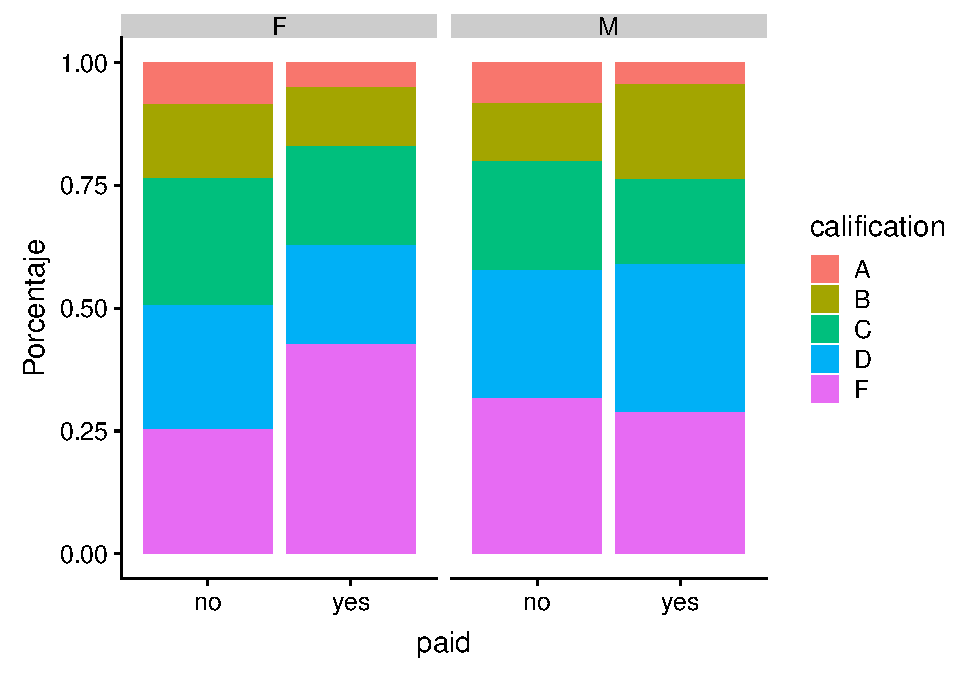
\includegraphics{Practica2_files/figure-latex/unnamed-chunk-26-1.pdf}

\begin{Shaded}
\begin{Highlighting}[]
\KeywordTok{ggplot}\NormalTok{(students,}\KeywordTok{aes}\NormalTok{(}\DataTypeTok{x=}\NormalTok{paid,}\DataTypeTok{fill=}\NormalTok{calification))}\OperatorTok{+}\KeywordTok{geom_bar}\NormalTok{()}\OperatorTok{+}\KeywordTok{ylab}\NormalTok{(}\StringTok{"Frecuencia"}\NormalTok{)}\OperatorTok{+}\KeywordTok{facet_wrap}\NormalTok{(}\OperatorTok{~}\NormalTok{sex )}
\end{Highlighting}
\end{Shaded}

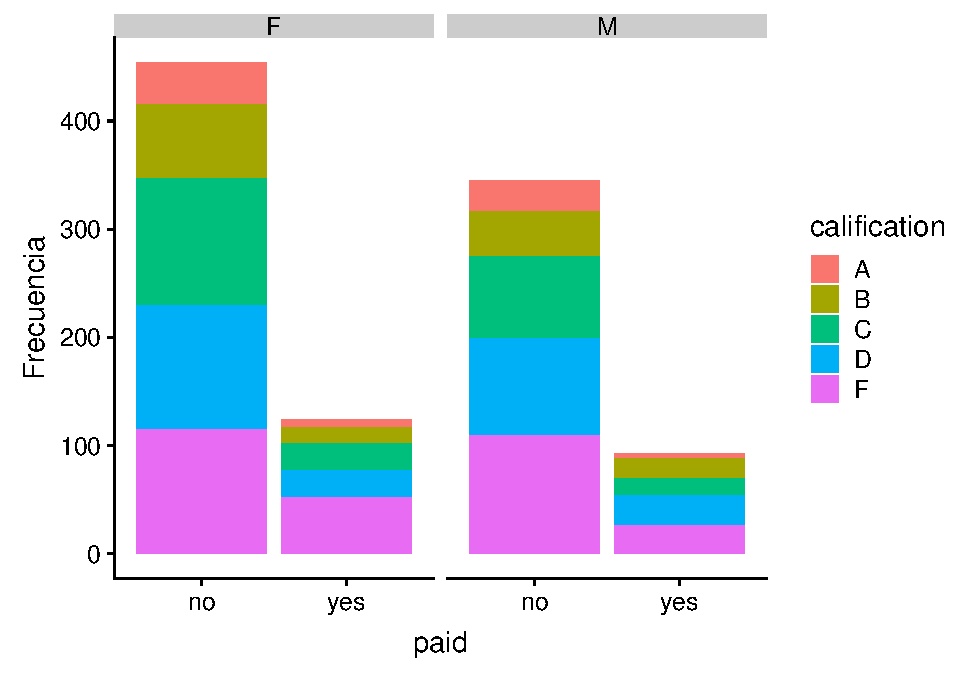
\includegraphics{Practica2_files/figure-latex/unnamed-chunk-26-2.pdf}

\begin{Shaded}
\begin{Highlighting}[]
\KeywordTok{ggplot}\NormalTok{(students,}\KeywordTok{aes}\NormalTok{(}\DataTypeTok{x=}\NormalTok{famsup,}\DataTypeTok{fill=}\NormalTok{calification))}\OperatorTok{+}\KeywordTok{geom_bar}\NormalTok{(}\DataTypeTok{position=}\StringTok{"fill"}\NormalTok{)}\OperatorTok{+}\KeywordTok{ylab}\NormalTok{(}\StringTok{"Porcentaje"}\NormalTok{)}\OperatorTok{+}\KeywordTok{facet_wrap}\NormalTok{(}\OperatorTok{~}\NormalTok{sex )}
\end{Highlighting}
\end{Shaded}

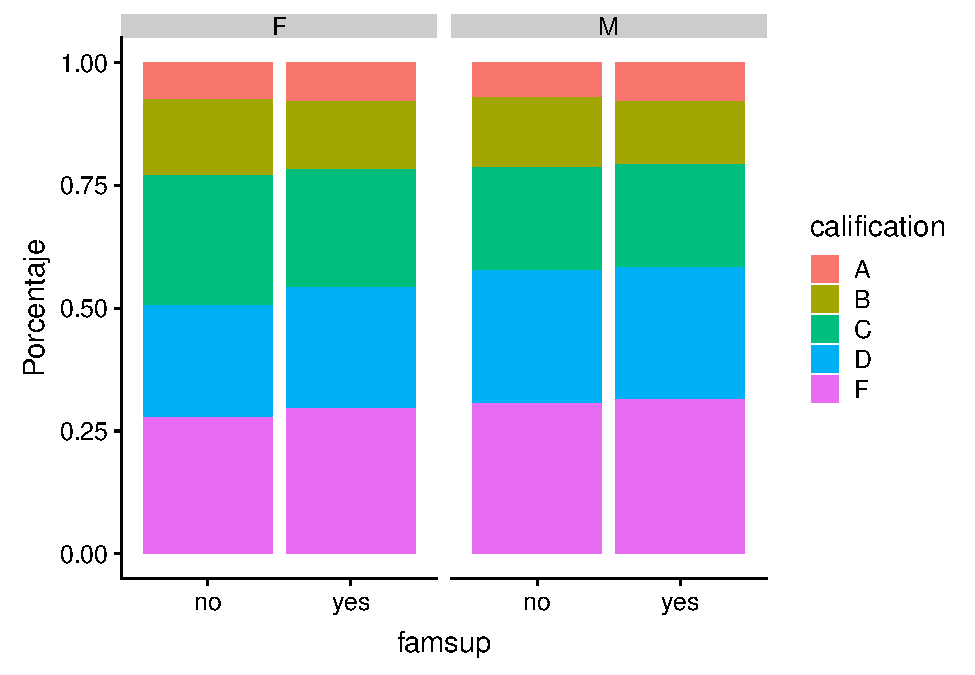
\includegraphics{Practica2_files/figure-latex/unnamed-chunk-27-1.pdf}

\begin{Shaded}
\begin{Highlighting}[]
\KeywordTok{ggplot}\NormalTok{(students,}\KeywordTok{aes}\NormalTok{(}\DataTypeTok{x=}\NormalTok{famsup,}\DataTypeTok{fill=}\NormalTok{calification))}\OperatorTok{+}\KeywordTok{geom_bar}\NormalTok{()}\OperatorTok{+}\KeywordTok{ylab}\NormalTok{(}\StringTok{"Frecuencia"}\NormalTok{)}\OperatorTok{+}\KeywordTok{facet_wrap}\NormalTok{(}\OperatorTok{~}\NormalTok{sex )}
\end{Highlighting}
\end{Shaded}

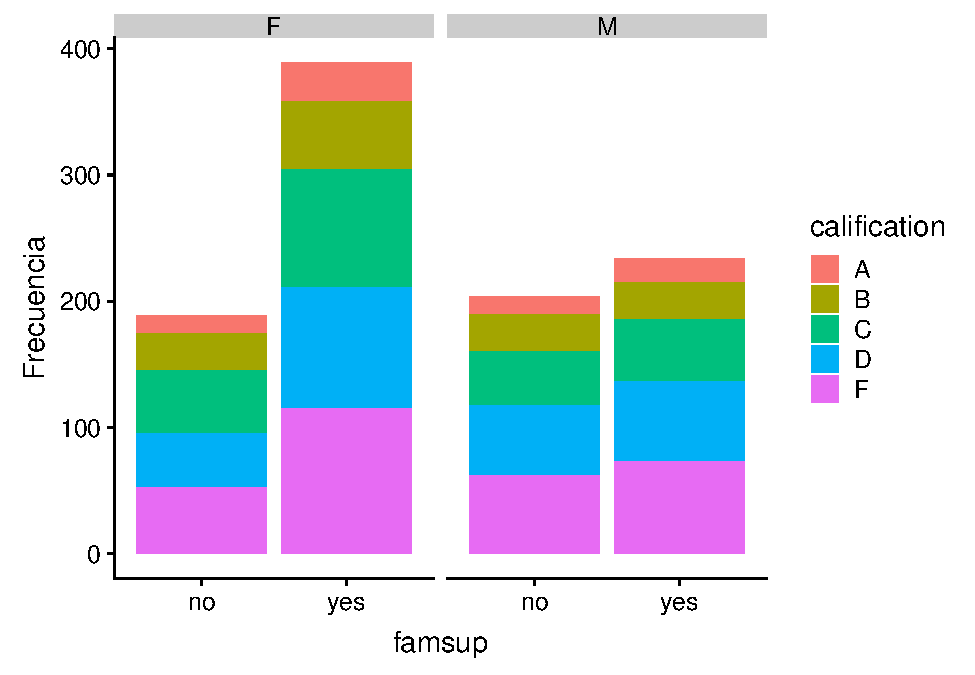
\includegraphics{Practica2_files/figure-latex/unnamed-chunk-27-2.pdf}

\hypertarget{comprobacion-de-la-normalidad-y-homogeneidad-de-la-varianza}{%
\subsubsection{Comprobación de la normalidad y homogeneidad de la
varianza}\label{comprobacion-de-la-normalidad-y-homogeneidad-de-la-varianza}}

Para la comprobación de que los valores que toman nuestras variables
cuantitativas provienen de una población distribuida normalmente,
utilizaremos la prueba de normalidad de Anderson-Darling. Así, se
comprueba que para que cada prueba se obtiene un p-valor superior al
nivel de significación prefijado α \(alpha\) = 0,05. Si esto se cumple,
entonces se considera que la variable en cuestión sigue una distribución
normal.

\begin{Shaded}
\begin{Highlighting}[]
\CommentTok{# Tests de normalidad }
\KeywordTok{library}\NormalTok{(nortest)}

\CommentTok{# Función que aplica distintos test de homogeneidad sobre los datos de entrada}
\NormalTok{normTest <-}\StringTok{ }\ControlFlowTok{function}\NormalTok{(data, name, }\DataTypeTok{alpha =} \FloatTok{0.05}\NormalTok{) \{}
\NormalTok{  ad_val =}\StringTok{ }\NormalTok{(}\KeywordTok{ad.test}\NormalTok{(data)}\OperatorTok{$}\NormalTok{p.value }\OperatorTok{>}\StringTok{ }\NormalTok{alpha) }\CommentTok{# Anderson-Darling test}
\NormalTok{  ks_val =}\StringTok{ }\NormalTok{(}\KeywordTok{ks.test}\NormalTok{(data, pnorm, }\KeywordTok{mean}\NormalTok{(data), }\KeywordTok{sd}\NormalTok{(data))}\OperatorTok{$}\NormalTok{p.value }\OperatorTok{>}\StringTok{ }\NormalTok{alpha) }\CommentTok{# Kolmogorov-Smirnov test}
\NormalTok{  sh_val =}\StringTok{ }\NormalTok{(}\KeywordTok{shapiro.test}\NormalTok{(data)}\OperatorTok{$}\NormalTok{p.value }\OperatorTok{>}\StringTok{ }\NormalTok{alpha) }\CommentTok{# Shapiro test}
\NormalTok{  csv_val =}\StringTok{ }\NormalTok{(}\KeywordTok{cvm.test}\NormalTok{(data)}\OperatorTok{$}\NormalTok{p.value }\OperatorTok{>}\StringTok{ }\NormalTok{alpha) }\CommentTok{# Cramer-von Mises test}
  \KeywordTok{cat}\NormalTok{(name)}
  \KeywordTok{cat}\NormalTok{(}\StringTok{"}\CharTok{\textbackslash{}t}\StringTok{"}\NormalTok{)}
  \KeywordTok{cat}\NormalTok{(ad_val,ks_val,sh_val,csv_val,}\StringTok{"}\CharTok{\textbackslash{}t}\StringTok{"}\NormalTok{)}
  \KeywordTok{cat}\NormalTok{(}\StringTok{"}\CharTok{\textbackslash{}n}\StringTok{"}\NormalTok{)}
\NormalTok{\}}
\end{Highlighting}
\end{Shaded}

\begin{Shaded}
\begin{Highlighting}[]
\NormalTok{col.names =}\StringTok{ }\KeywordTok{colnames}\NormalTok{(students)}
\KeywordTok{cat}\NormalTok{(}\StringTok{"Distribucion normal: }\CharTok{\textbackslash{}n}\StringTok{"}\NormalTok{)}
\end{Highlighting}
\end{Shaded}

\begin{verbatim}
## Distribucion normal:
\end{verbatim}

\begin{Shaded}
\begin{Highlighting}[]
\ControlFlowTok{for}\NormalTok{ (i }\ControlFlowTok{in} \DecValTok{1}\OperatorTok{:}\KeywordTok{ncol}\NormalTok{(students)) \{}
  \ControlFlowTok{if}\NormalTok{ (}\KeywordTok{is.integer}\NormalTok{(students[,i]) }\OperatorTok{|}\StringTok{ }\KeywordTok{is.numeric}\NormalTok{(students[,i])) \{}
    \KeywordTok{normTest}\NormalTok{(students[,i], col.names[i])}
\NormalTok{  \}}
\NormalTok{\}}
\end{Highlighting}
\end{Shaded}

\begin{verbatim}
## age  FALSE FALSE FALSE FALSE     
## Medu FALSE FALSE FALSE FALSE     
## Fedu FALSE FALSE FALSE FALSE     
## traveltime   FALSE FALSE FALSE FALSE     
## studytime    FALSE FALSE FALSE FALSE     
## failures FALSE FALSE FALSE FALSE     
## famrel   FALSE FALSE FALSE FALSE     
## freetime FALSE FALSE FALSE FALSE     
## goout    FALSE FALSE FALSE FALSE     
## Dalc FALSE FALSE FALSE FALSE     
## Walc FALSE FALSE FALSE FALSE     
## health   FALSE FALSE FALSE FALSE     
## absences FALSE FALSE FALSE FALSE     
## G1   FALSE FALSE FALSE FALSE     
## G2   FALSE FALSE FALSE FALSE     
## G3   FALSE FALSE FALSE FALSE     
## score    FALSE FALSE FALSE FALSE     
\end{verbatim}

Luego a la vista de los resultados obtenidos en los diferentes tests de
normalidad, vemos que ninguna de las variables numéricas que tenemos en
nuestro juego de datos sigue una distribución normal con respecto al
conjunto total de los datos.

Ahora vamos a ver si estas variables numéricas siguen una distribución
normal en cada uno de los grupos que hemos separado para realizar
nuestro análisis. Es decir, vamos a ver si:

Hemos visto que las notas registradas no siguen una distrubución normal
para el conjunto total de los datos pero, seguirán una distribución
normal en el conjunto de hombres o de mujeres? ¿Y en el caso de que el
tiempo de estudio sea de más de 3 horas o de menos? ¿Y de los alumnos
mayores de 16 años o menores? ¿Y si separamos los datos entre alumnos
que reciben clases particulares pagadas y no? ¿Y si reciben ayuda
extraescolar de familia o en el colegio?

\begin{Shaded}
\begin{Highlighting}[]
\KeywordTok{normTest}\NormalTok{(students.female[,}\KeywordTok{c}\NormalTok{(}\StringTok{"score"}\NormalTok{)], }\StringTok{"score~female"}\NormalTok{)}
\end{Highlighting}
\end{Shaded}

\begin{verbatim}
## score~female FALSE TRUE FALSE FALSE  
\end{verbatim}

\begin{Shaded}
\begin{Highlighting}[]
\KeywordTok{normTest}\NormalTok{(students.male[,}\KeywordTok{c}\NormalTok{(}\StringTok{"score"}\NormalTok{)], }\StringTok{"score~male"}\NormalTok{)}
\end{Highlighting}
\end{Shaded}

\begin{verbatim}
## score~male   FALSE TRUE FALSE FALSE  
\end{verbatim}

\begin{Shaded}
\begin{Highlighting}[]
\KeywordTok{normTest}\NormalTok{(students.studytime[,}\KeywordTok{c}\NormalTok{(}\StringTok{"score"}\NormalTok{)], }\StringTok{"score~studytime"}\NormalTok{)}
\end{Highlighting}
\end{Shaded}

\begin{verbatim}
## score~studytime  TRUE TRUE FALSE TRUE    
\end{verbatim}

\begin{Shaded}
\begin{Highlighting}[]
\KeywordTok{normTest}\NormalTok{(students.nostudytime[,}\KeywordTok{c}\NormalTok{(}\StringTok{"score"}\NormalTok{)], }\StringTok{"score~nostudytime"}\NormalTok{)}
\end{Highlighting}
\end{Shaded}

\begin{verbatim}
## score~nostudytime    FALSE FALSE FALSE FALSE     
\end{verbatim}

\begin{Shaded}
\begin{Highlighting}[]
\KeywordTok{normTest}\NormalTok{(students.mayores[,}\KeywordTok{c}\NormalTok{(}\StringTok{"score"}\NormalTok{)], }\StringTok{"score~mayores"}\NormalTok{)}
\end{Highlighting}
\end{Shaded}

\begin{verbatim}
## score~mayores    FALSE TRUE FALSE FALSE  
\end{verbatim}

\begin{Shaded}
\begin{Highlighting}[]
\KeywordTok{normTest}\NormalTok{(students.menores[,}\KeywordTok{c}\NormalTok{(}\StringTok{"score"}\NormalTok{)], }\StringTok{"score~menores"}\NormalTok{)}
\end{Highlighting}
\end{Shaded}

\begin{verbatim}
## score~menores    TRUE TRUE TRUE TRUE     
\end{verbatim}

\begin{Shaded}
\begin{Highlighting}[]
\KeywordTok{normTest}\NormalTok{(students.paid[,}\KeywordTok{c}\NormalTok{(}\StringTok{"score"}\NormalTok{)], }\StringTok{"score~paid"}\NormalTok{)}
\end{Highlighting}
\end{Shaded}

\begin{verbatim}
## score~paid   TRUE TRUE TRUE TRUE     
\end{verbatim}

\begin{Shaded}
\begin{Highlighting}[]
\KeywordTok{normTest}\NormalTok{(students.nopaid[,}\KeywordTok{c}\NormalTok{(}\StringTok{"score"}\NormalTok{)], }\StringTok{"score~nopaid"}\NormalTok{)}
\end{Highlighting}
\end{Shaded}

\begin{verbatim}
## score~nopaid FALSE FALSE FALSE FALSE     
\end{verbatim}

\begin{Shaded}
\begin{Highlighting}[]
\KeywordTok{normTest}\NormalTok{(students.schoolsup[,}\KeywordTok{c}\NormalTok{(}\StringTok{"score"}\NormalTok{)], }\StringTok{"score~schoolsup"}\NormalTok{)}
\end{Highlighting}
\end{Shaded}

\begin{verbatim}
## score~schoolsup  TRUE TRUE TRUE TRUE     
\end{verbatim}

\begin{Shaded}
\begin{Highlighting}[]
\KeywordTok{normTest}\NormalTok{(students.noschoolsup[,}\KeywordTok{c}\NormalTok{(}\StringTok{"score"}\NormalTok{)], }\StringTok{"score~noschoolsup"}\NormalTok{)}
\end{Highlighting}
\end{Shaded}

\begin{verbatim}
## score~noschoolsup    FALSE FALSE FALSE FALSE     
\end{verbatim}

\begin{Shaded}
\begin{Highlighting}[]
\KeywordTok{normTest}\NormalTok{(students.famsup[,}\KeywordTok{c}\NormalTok{(}\StringTok{"score"}\NormalTok{)], }\StringTok{"score~famsup"}\NormalTok{)}
\end{Highlighting}
\end{Shaded}

\begin{verbatim}
## score~famsup FALSE TRUE FALSE TRUE   
\end{verbatim}

\begin{Shaded}
\begin{Highlighting}[]
\KeywordTok{normTest}\NormalTok{(students.nofamsup[,}\KeywordTok{c}\NormalTok{(}\StringTok{"score"}\NormalTok{)], }\StringTok{"score~nofamsup"}\NormalTok{)}
\end{Highlighting}
\end{Shaded}

\begin{verbatim}
## score~nofamsup   FALSE TRUE FALSE FALSE  
\end{verbatim}

Según los resultados obtenidos vemos que, para los alumnos menores de 16
años, las notas medias sí siguen una distribución normal, y para el caso
de los que reciben clases particulares pagadas también así como para
aquellos que reciben apoyo educativo adicional . Para el caso de las
alumnas femeninas,y de los grupos que reciben o no reciben ayuda
extraescolar familiar, el test de Kolmogorov sí indica que las variables
de notas medias siguen una distribución normal

\begin{quote}
Se utiliza el test de Fligner-Killeen, al no tener normalidad en los
datos. Se utilizaría el test Levene cuando hay normalidad en los datos.
\end{quote}

Vamos a estudiar ahora la homogeneidad de la varianza para los
diferentes grupos que queremos analizar. En primer lugar vamos a
analizar la homocedasticidad entre niños y niñas. Vimos en el apartado
anterior que esta variable no sigue una distribución normal para estos
grupos, luego para realizar nuestro análisis utilizaremos el test de
Fligner-Killeen.

\begin{Shaded}
\begin{Highlighting}[]
\KeywordTok{fligner.test}\NormalTok{(score }\OperatorTok{~}\StringTok{ }\NormalTok{sex, }\DataTypeTok{data =}\NormalTok{ students)}
\end{Highlighting}
\end{Shaded}

\begin{verbatim}
## 
##  Fligner-Killeen test of homogeneity of variances
## 
## data:  score by sex
## Fligner-Killeen:med chi-squared = 0.18014, df = 1, p-value =
## 0.6713
\end{verbatim}

Vemos, por tanto, que el valor de p obtenido (p-value) es mayor que 0,05
luego esto indica que no se observa diferencia significativa entre las
varianzas por grupos de sexo.

Vamos a aplicar el test de Levene para ver que resultado obtenemos en
este caso:

\begin{Shaded}
\begin{Highlighting}[]
\KeywordTok{leveneTest}\NormalTok{(score }\OperatorTok{~}\StringTok{ }\NormalTok{sex, }\DataTypeTok{data =}\NormalTok{ students)}
\end{Highlighting}
\end{Shaded}

\begin{verbatim}
## Levene's Test for Homogeneity of Variance (center = median)
##         Df F value Pr(>F)
## group    1   0.141 0.7074
##       1014
\end{verbatim}

Para este caso también se cumpliría que el valor de p es mayor de 0,05
luego también indicaría que no existe diferencia significativa entre las
varianzas

Veamos ahora cómo se distribuye la varianza para la media escolar entre
los grupos de alumnos que reciben clases privadas de las asignaturas.
Nuevamente, como estos valores no siguen una distribución normal,
utilizaremos el test de Fligner-Killeen

\begin{Shaded}
\begin{Highlighting}[]
\KeywordTok{fligner.test}\NormalTok{(score }\OperatorTok{~}\StringTok{ }\NormalTok{paid, }\DataTypeTok{data =}\NormalTok{ students)}
\end{Highlighting}
\end{Shaded}

\begin{verbatim}
## 
##  Fligner-Killeen test of homogeneity of variances
## 
## data:  score by paid
## Fligner-Killeen:med chi-squared = 0.95484, df = 1, p-value =
## 0.3285
\end{verbatim}

Nuevamente, vemos que el valor de p es mayor de 0.05, luego podemos
concluir que las varianzas están homogéneamente distrubuidas.

Si aplicamos es test de Levene

\begin{Shaded}
\begin{Highlighting}[]
\KeywordTok{leveneTest}\NormalTok{(score }\OperatorTok{~}\StringTok{ }\NormalTok{paid, }\DataTypeTok{data =}\NormalTok{ students)}
\end{Highlighting}
\end{Shaded}

\begin{verbatim}
## Levene's Test for Homogeneity of Variance (center = median)
##         Df F value Pr(>F)
## group    1  1.0994 0.2946
##       1014
\end{verbatim}

Vemos también el mismo resultado

Si ahora analizamos las distribuciones atendiendo a si reciben clases
estraescolares o ayudas de sus padres, vamos a ver qué obtenemos,
nuevamente aplicando el test de Fligner-Killeen por la falta de
normalidad en nuestros datos.

\begin{Shaded}
\begin{Highlighting}[]
\KeywordTok{fligner.test}\NormalTok{(score }\OperatorTok{~}\StringTok{ }\NormalTok{schoolsup, }\DataTypeTok{data =}\NormalTok{ students)}
\end{Highlighting}
\end{Shaded}

\begin{verbatim}
## 
##  Fligner-Killeen test of homogeneity of variances
## 
## data:  score by schoolsup
## Fligner-Killeen:med chi-squared = 13.884, df = 1, p-value =
## 0.0001945
\end{verbatim}

En este caso vemos que el valor de p obtenido es menor que 0,05 luego
vemos que la variable score (que recoge las medias de todas las notas
obtenidas) presenta varianzas estadísticamente diferentes para los
grupos de alumnos que reciben ayuda extraescolar o no en el colegio.

Vamos a ver qué resultados obtenemos para este caso utilizando el test
de Levene

\begin{Shaded}
\begin{Highlighting}[]
\KeywordTok{leveneTest}\NormalTok{(score }\OperatorTok{~}\StringTok{ }\NormalTok{schoolsup, }\DataTypeTok{data =}\NormalTok{ students)}
\end{Highlighting}
\end{Shaded}

\begin{verbatim}
## Levene's Test for Homogeneity of Variance (center = median)
##         Df F value    Pr(>F)    
## group    1   14.54 0.0001455 ***
##       1014                      
## ---
## Signif. codes:  0 '***' 0.001 '**' 0.01 '*' 0.05 '.' 0.1 ' ' 1
\end{verbatim}

Nuevamente el valor es menor que 0.05

Analicemos ahora cómo se distribuye la varianza de las notas medias para
los grupos de alumnos que reciben ayuda suplementaria en casa.
Nuevamente, usamos el test de Fligner-Killeen

\begin{Shaded}
\begin{Highlighting}[]
\KeywordTok{fligner.test}\NormalTok{(score }\OperatorTok{~}\StringTok{ }\NormalTok{famsup, }\DataTypeTok{data =}\NormalTok{ students)}
\end{Highlighting}
\end{Shaded}

\begin{verbatim}
## 
##  Fligner-Killeen test of homogeneity of variances
## 
## data:  score by famsup
## Fligner-Killeen:med chi-squared = 1.0762, df = 1, p-value = 0.2996
\end{verbatim}

En este caso, se observa que el valor de p (p-value) es mayor de 0,05
luego podemos concluir que las varianzas son homogéneas para estos
grupos de estudiantes

Analicemos cómo se distribuye la varianza de las notas medias por los
diferentes grupos de edad, entre los alumnos menores de 16 y los mayores
de 16

\begin{Shaded}
\begin{Highlighting}[]
\NormalTok{a <-}\StringTok{ }\NormalTok{students[students}\OperatorTok{$}\NormalTok{age }\OperatorTok{<}\StringTok{ }\DecValTok{16}\NormalTok{,}\StringTok{"score"}\NormalTok{]}
\NormalTok{b <-}\StringTok{ }\NormalTok{students[students}\OperatorTok{$}\NormalTok{age }\OperatorTok{>=}\StringTok{ }\DecValTok{16}\NormalTok{,}\StringTok{"score"}\NormalTok{]}
\KeywordTok{fligner.test}\NormalTok{(}\DataTypeTok{x =} \KeywordTok{list}\NormalTok{(a,b))}
\end{Highlighting}
\end{Shaded}

\begin{verbatim}
## 
##  Fligner-Killeen test of homogeneity of variances
## 
## data:  list(a, b)
## Fligner-Killeen:med chi-squared = 5.3901, df = 1, p-value =
## 0.02025
\end{verbatim}

El valor de p que obtenemos es menor que 0.05 lyego rechazamos la
hipótesis de homocedasticidad y concluimos que la variable score tiene
varianzas estadísticamente diferentes para los alumnos menores de 16 y
los mayores de 16.

Por último estudiaremos la distribución de la varianza para los grupos
de alumnos que estudian más o menos de 3 horas.

\begin{Shaded}
\begin{Highlighting}[]
\NormalTok{a <-}\StringTok{ }\NormalTok{students[students}\OperatorTok{$}\NormalTok{studytime }\OperatorTok{<}\StringTok{ }\DecValTok{3}\NormalTok{,}\StringTok{"score"}\NormalTok{]}
\NormalTok{b <-}\StringTok{ }\NormalTok{students[students}\OperatorTok{$}\NormalTok{studytime }\OperatorTok{>=}\StringTok{ }\DecValTok{3}\NormalTok{,}\StringTok{"score"}\NormalTok{]}
\KeywordTok{fligner.test}\NormalTok{(}\DataTypeTok{x =} \KeywordTok{list}\NormalTok{(a,b))}
\end{Highlighting}
\end{Shaded}

\begin{verbatim}
## 
##  Fligner-Killeen test of homogeneity of variances
## 
## data:  list(a, b)
## Fligner-Killeen:med chi-squared = 0.0058552, df = 1, p-value =
## 0.939
\end{verbatim}

El valor de p es mayor de 0.05 luego podemos concluir que sí existe
homogeneidad de la varianza

Vamos a representar los histogramas de estas variables

\begin{Shaded}
\begin{Highlighting}[]
\NormalTok{plotNormHistogram <-}\StringTok{ }\ControlFlowTok{function}\NormalTok{(data, name) \{}
    \KeywordTok{qqnorm}\NormalTok{(data,}\DataTypeTok{main =} \KeywordTok{paste}\NormalTok{(}\StringTok{"Normal Q-Q Plot for "}\NormalTok{,name))}
    \KeywordTok{qqline}\NormalTok{(data,}\DataTypeTok{col=}\StringTok{"red"}\NormalTok{)}
    \KeywordTok{hist}\NormalTok{(data, }
      \DataTypeTok{main=}\KeywordTok{paste}\NormalTok{(}\StringTok{"Histogram for "}\NormalTok{, name), }
      \DataTypeTok{xlab=}\NormalTok{name, }\DataTypeTok{freq =} \OtherTok{FALSE}\NormalTok{)}
\NormalTok{\}}
\end{Highlighting}
\end{Shaded}

\begin{Shaded}
\begin{Highlighting}[]
\KeywordTok{par}\NormalTok{(}\DataTypeTok{mfrow=}\KeywordTok{c}\NormalTok{(}\DecValTok{2}\NormalTok{,}\DecValTok{2}\NormalTok{))}
\ControlFlowTok{for}\NormalTok{(i }\ControlFlowTok{in} \DecValTok{1}\OperatorTok{:}\KeywordTok{ncol}\NormalTok{(students)) \{}
  \ControlFlowTok{if}\NormalTok{ (}\KeywordTok{is.numeric}\NormalTok{(students[,i]))\{}
    \KeywordTok{plotNormHistogram}\NormalTok{(students[,i], }\KeywordTok{colnames}\NormalTok{(students)[i])}
\NormalTok{  \}}
\NormalTok{\}}
\end{Highlighting}
\end{Shaded}

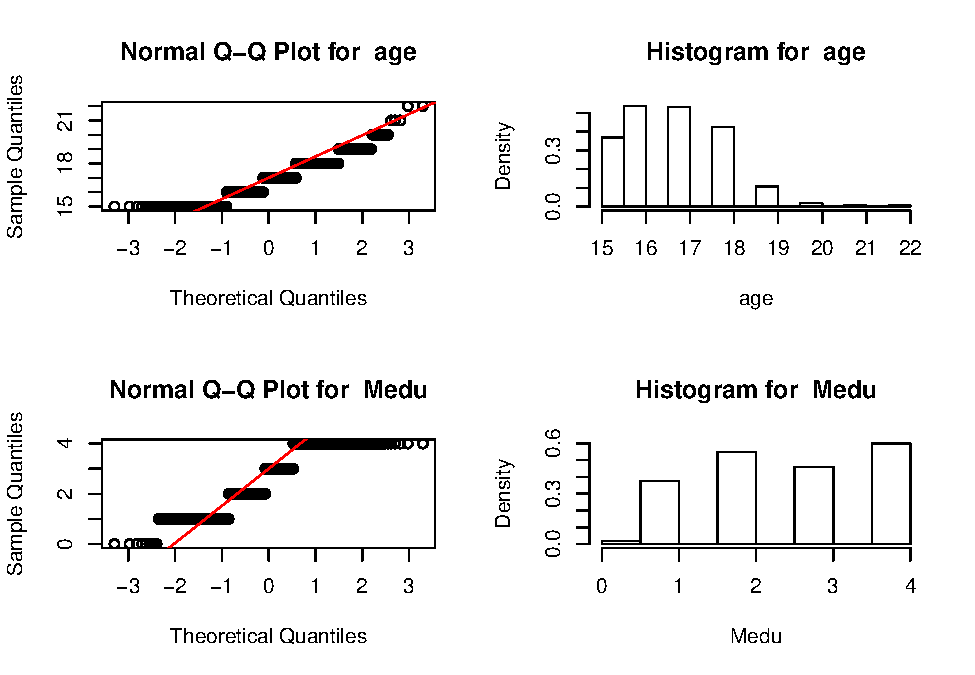
\includegraphics{Practica2_files/figure-latex/unnamed-chunk-41-1.pdf}
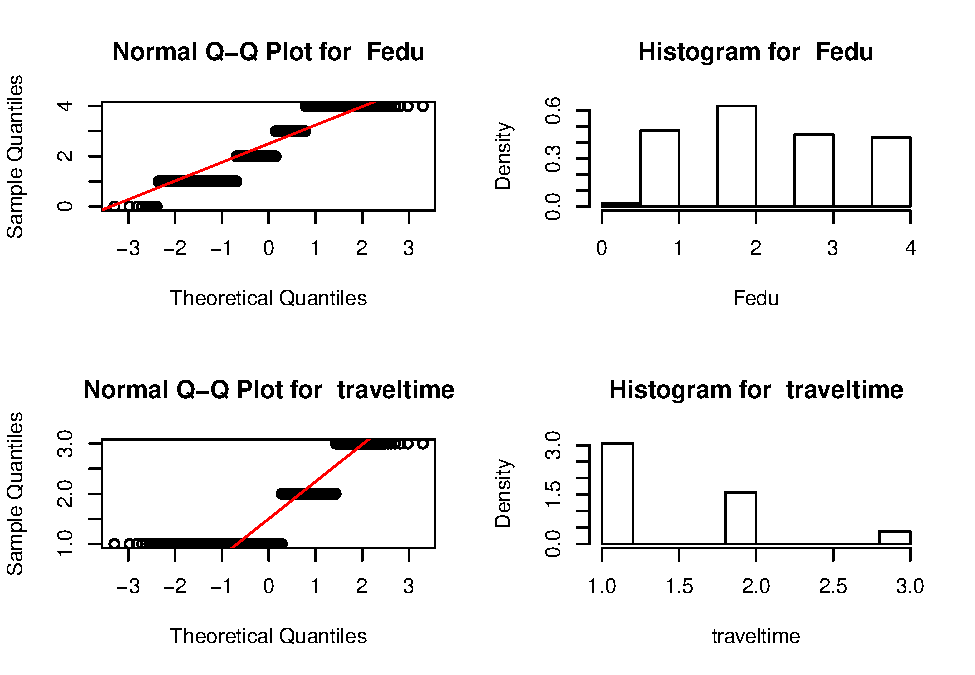
\includegraphics{Practica2_files/figure-latex/unnamed-chunk-41-2.pdf}
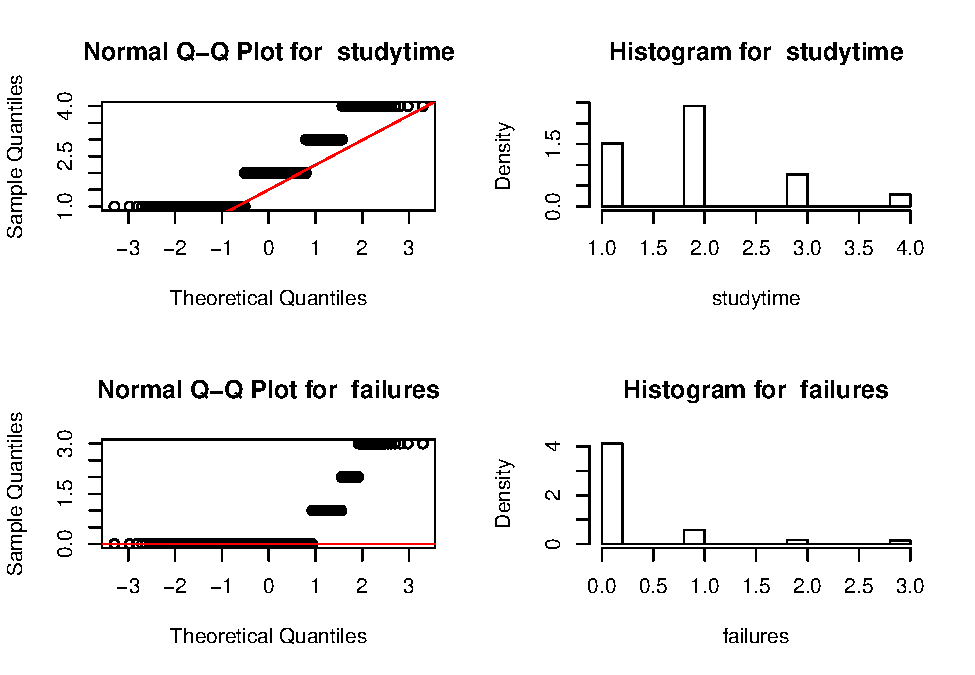
\includegraphics{Practica2_files/figure-latex/unnamed-chunk-41-3.pdf}
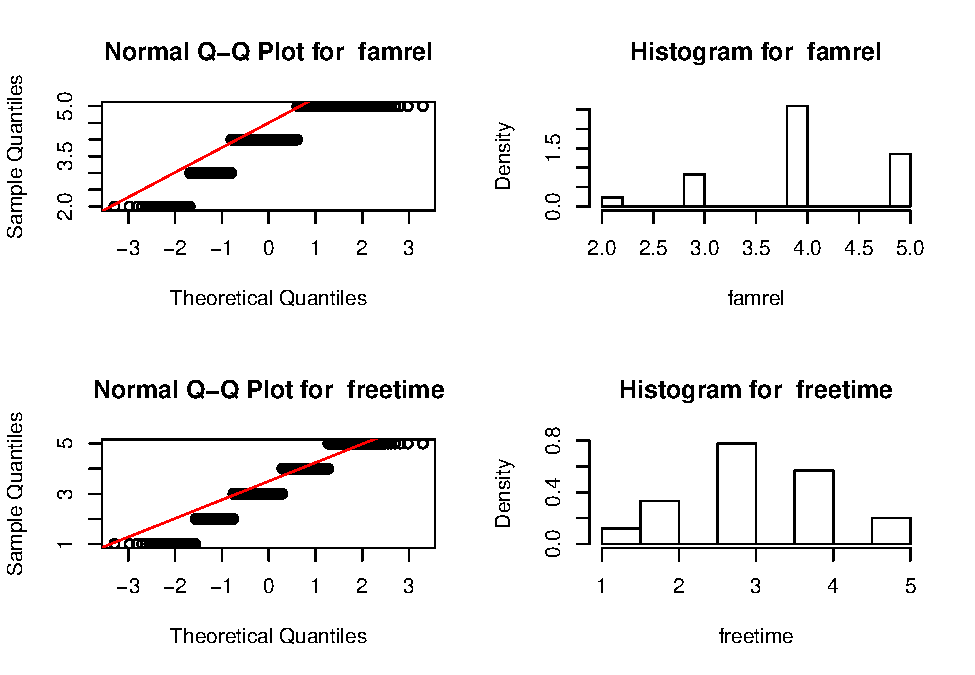
\includegraphics{Practica2_files/figure-latex/unnamed-chunk-41-4.pdf}
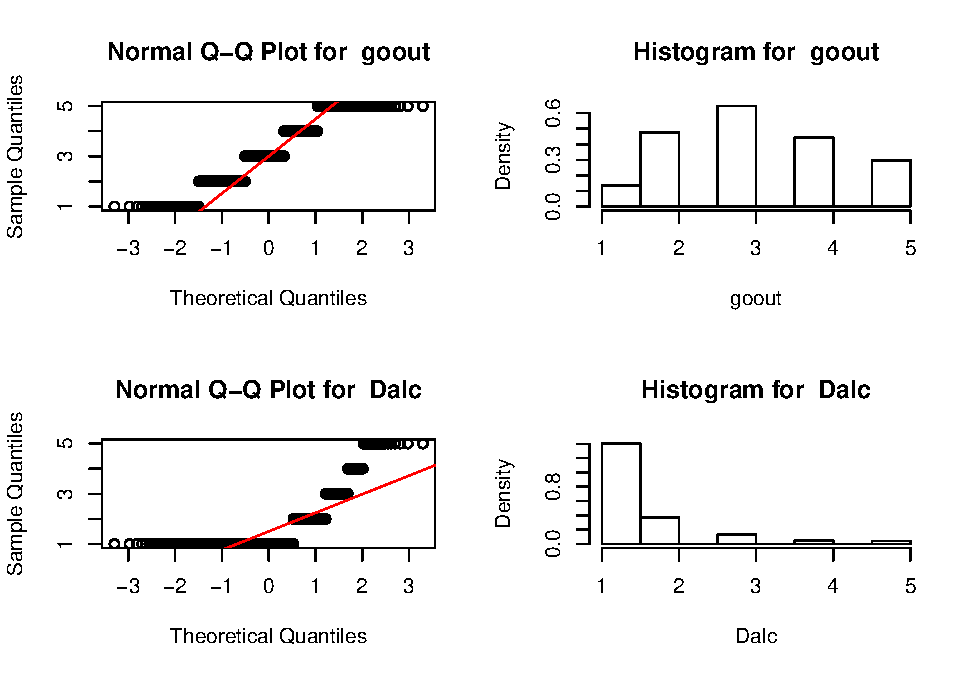
\includegraphics{Practica2_files/figure-latex/unnamed-chunk-41-5.pdf}
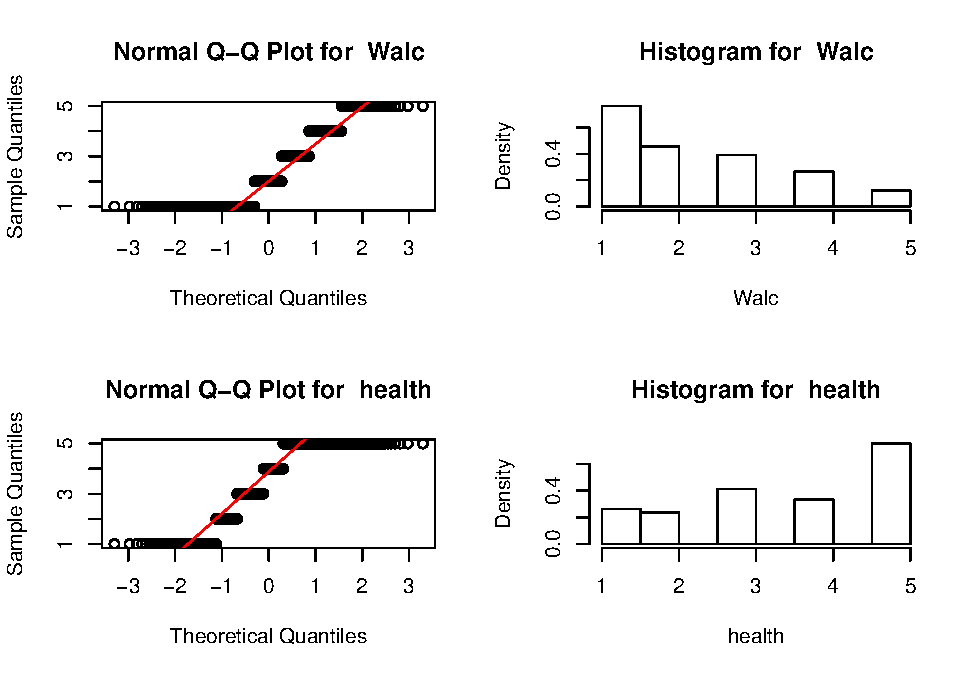
\includegraphics{Practica2_files/figure-latex/unnamed-chunk-41-6.pdf}
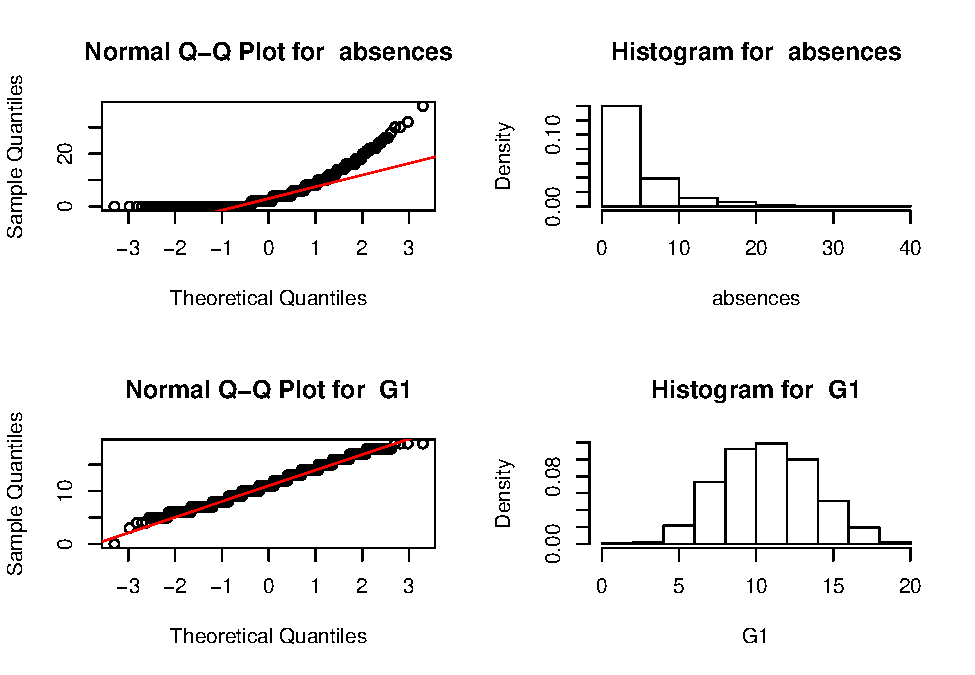
\includegraphics{Practica2_files/figure-latex/unnamed-chunk-41-7.pdf}
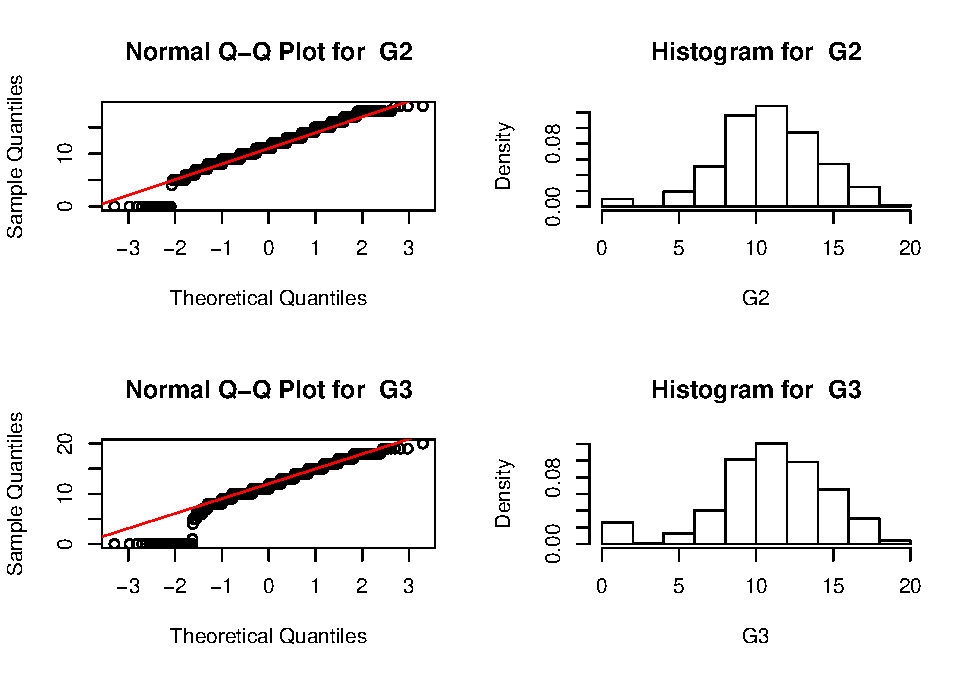
\includegraphics{Practica2_files/figure-latex/unnamed-chunk-41-8.pdf}
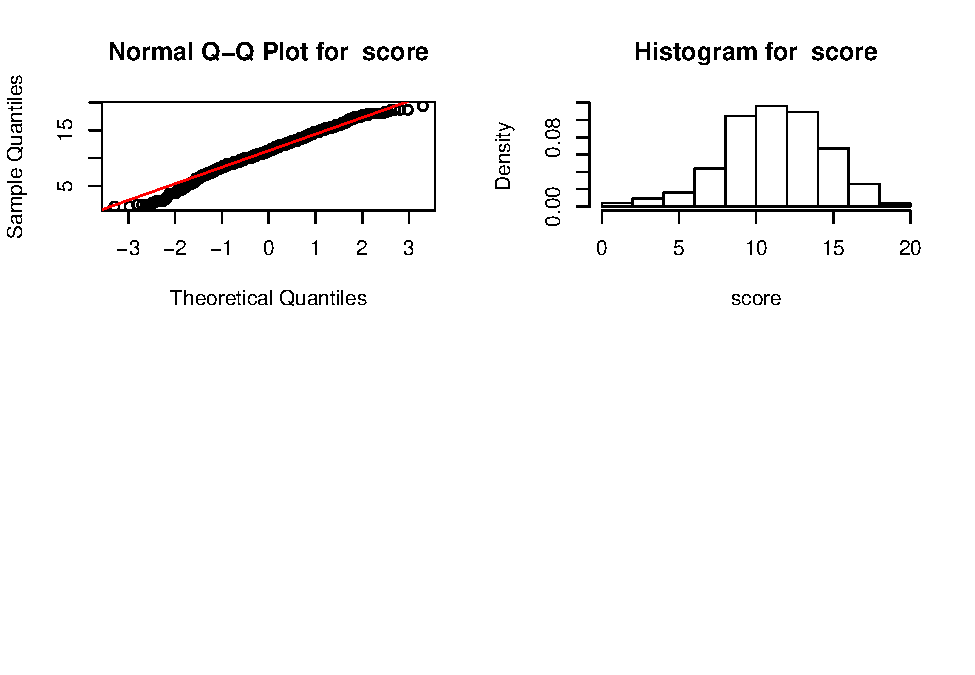
\includegraphics{Practica2_files/figure-latex/unnamed-chunk-41-9.pdf}

\begin{Shaded}
\begin{Highlighting}[]
\KeywordTok{par}\NormalTok{(}\DataTypeTok{mfrow=}\KeywordTok{c}\NormalTok{(}\DecValTok{2}\NormalTok{,}\DecValTok{2}\NormalTok{))}
\KeywordTok{plotNormHistogram}\NormalTok{(students.female[,}\KeywordTok{c}\NormalTok{(}\StringTok{"score"}\NormalTok{)], }\StringTok{"score~sex"}\NormalTok{)}
\KeywordTok{plotNormHistogram}\NormalTok{(students.male[,}\KeywordTok{c}\NormalTok{(}\StringTok{"score"}\NormalTok{)], }\StringTok{"score~sex"}\NormalTok{)}
\end{Highlighting}
\end{Shaded}

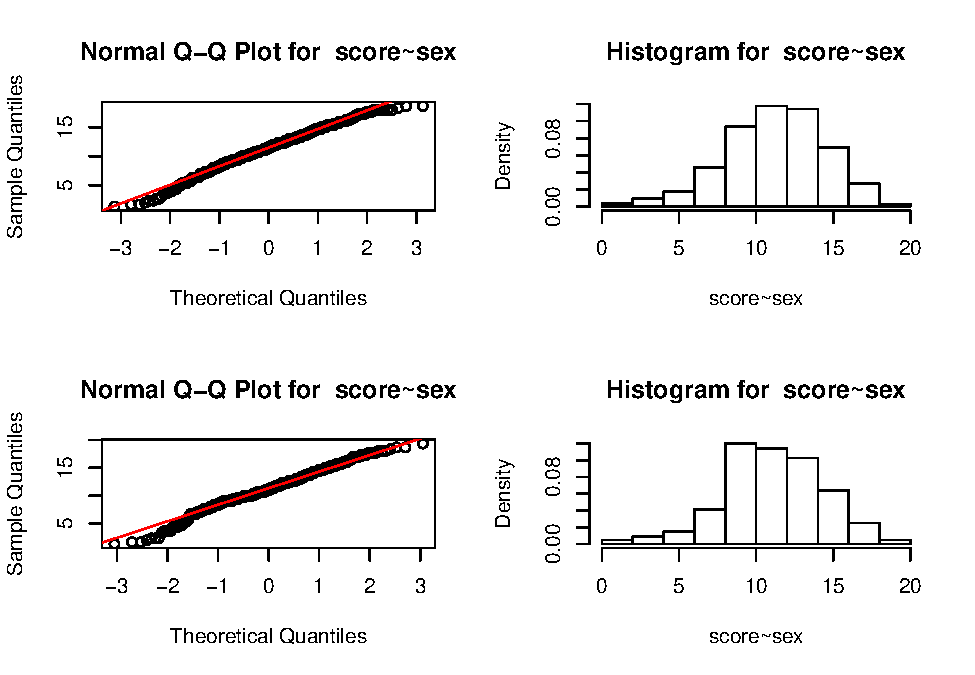
\includegraphics{Practica2_files/figure-latex/unnamed-chunk-42-1.pdf}

\begin{Shaded}
\begin{Highlighting}[]
\KeywordTok{plotNormHistogram}\NormalTok{(students.studytime[,}\KeywordTok{c}\NormalTok{(}\StringTok{"score"}\NormalTok{)], }\StringTok{"score~studytime"}\NormalTok{)}
\KeywordTok{plotNormHistogram}\NormalTok{(students.nostudytime[,}\KeywordTok{c}\NormalTok{(}\StringTok{"score"}\NormalTok{)], }\StringTok{"score~studytime"}\NormalTok{)}
\end{Highlighting}
\end{Shaded}

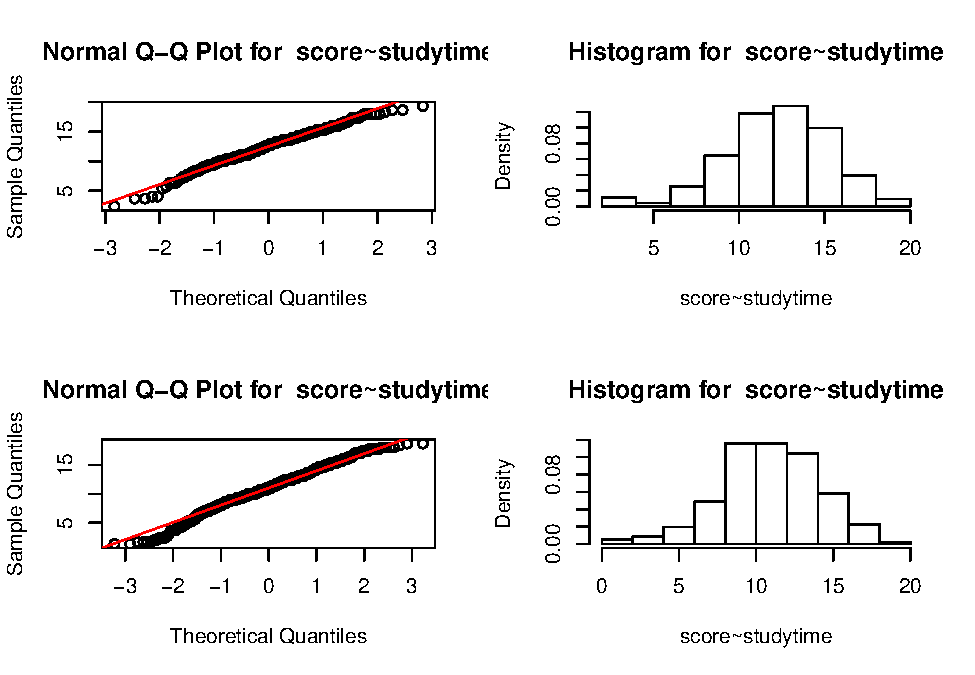
\includegraphics{Practica2_files/figure-latex/unnamed-chunk-42-2.pdf}

\begin{Shaded}
\begin{Highlighting}[]
\KeywordTok{plotNormHistogram}\NormalTok{(students.mayores[,}\KeywordTok{c}\NormalTok{(}\StringTok{"score"}\NormalTok{)], }\StringTok{"score~mayores"}\NormalTok{)}
\KeywordTok{plotNormHistogram}\NormalTok{(students.menores[,}\KeywordTok{c}\NormalTok{(}\StringTok{"score"}\NormalTok{)], }\StringTok{"score~menores"}\NormalTok{)}
\end{Highlighting}
\end{Shaded}

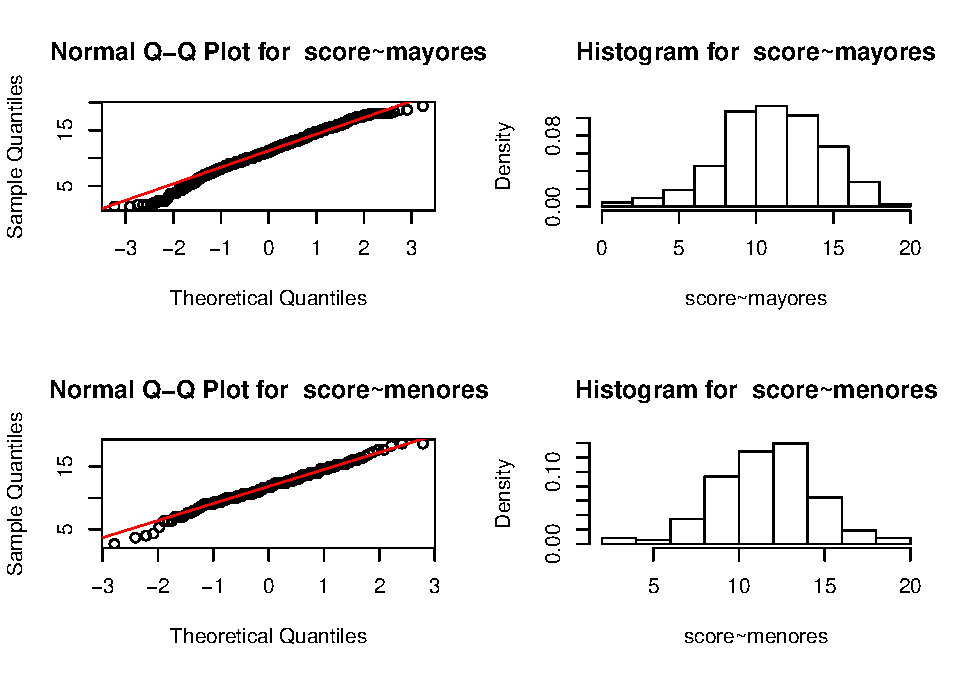
\includegraphics{Practica2_files/figure-latex/unnamed-chunk-42-3.pdf}

\hypertarget{pruebas-estadisticas}{%
\subsection{Pruebas estadísticas}\label{pruebas-estadisticas}}

Aplicación de pruebas estadísticas para comparar los grupos de datos. En
función de los datos y el objetivo del estudio, aplicar pruebas de
contraste de hipótesis, correlaciones, regresiones, etc. Aplicar al
menos tres métodos de análisis diferentes.

\hypertarget{correlaciones}{%
\subsubsection{Correlaciones}\label{correlaciones}}

\begin{Shaded}
\begin{Highlighting}[]
\NormalTok{color=}\KeywordTok{diverge_hcl}\NormalTok{(}\KeywordTok{length}\NormalTok{(students}\OperatorTok{$}\NormalTok{calification))[}\KeywordTok{rank}\NormalTok{(students}\OperatorTok{$}\NormalTok{calification)]}
\KeywordTok{pairs}\NormalTok{(}\OperatorTok{~}\StringTok{ }\NormalTok{G1 }\OperatorTok{+}\StringTok{ }\NormalTok{G2 }\OperatorTok{+}\StringTok{ }\NormalTok{G3 }\OperatorTok{+}\StringTok{ }\NormalTok{score, }\DataTypeTok{data =}\NormalTok{ students, }\DataTypeTok{pch =} \DecValTok{19}\NormalTok{, }\DataTypeTok{cex =} \FloatTok{0.5}\NormalTok{, }\DataTypeTok{lower.panel =} \OtherTok{NULL}\NormalTok{, }\DataTypeTok{col =}\NormalTok{ color)}
\KeywordTok{title}\NormalTok{(}\StringTok{"Correlación notas"}\NormalTok{)}
\end{Highlighting}
\end{Shaded}

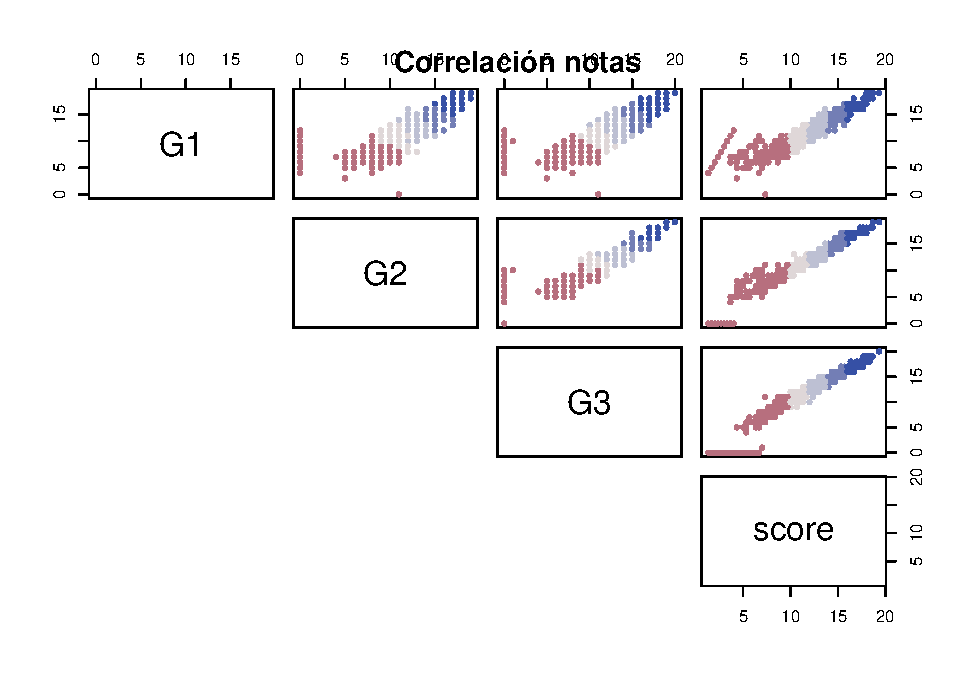
\includegraphics{Practica2_files/figure-latex/unnamed-chunk-43-1.pdf}

Luego, a la vista de estos diagramas, parece intuirse que existe una
posible relación lineal entre las notas de cada trimestre.

Como ya hemos visto que estas variables no siguen una distribución
normal, vamos a analizar la correlación utilizando el test de Spearman

\begin{Shaded}
\begin{Highlighting}[]
\KeywordTok{cor}\NormalTok{(}\DataTypeTok{x =}\NormalTok{ students}\OperatorTok{$}\NormalTok{G1, }\DataTypeTok{y =} \KeywordTok{log10}\NormalTok{(students}\OperatorTok{$}\NormalTok{G2), }\DataTypeTok{method =} \StringTok{"spearman"}\NormalTok{)}
\end{Highlighting}
\end{Shaded}

\begin{verbatim}
## [1] 0.8994989
\end{verbatim}

\begin{Shaded}
\begin{Highlighting}[]
\KeywordTok{cor}\NormalTok{(}\DataTypeTok{x =}\NormalTok{ students}\OperatorTok{$}\NormalTok{G1, }\DataTypeTok{y =} \KeywordTok{log10}\NormalTok{(students}\OperatorTok{$}\NormalTok{G3), }\DataTypeTok{method =} \StringTok{"spearman"}\NormalTok{)}
\end{Highlighting}
\end{Shaded}

\begin{verbatim}
## [1] 0.8881195
\end{verbatim}

\begin{Shaded}
\begin{Highlighting}[]
\KeywordTok{cor}\NormalTok{(}\DataTypeTok{x =}\NormalTok{ students}\OperatorTok{$}\NormalTok{G1, }\DataTypeTok{y =} \KeywordTok{log10}\NormalTok{(students}\OperatorTok{$}\NormalTok{score), }\DataTypeTok{method =} \StringTok{"spearman"}\NormalTok{)}
\end{Highlighting}
\end{Shaded}

\begin{verbatim}
## [1] 0.9523118
\end{verbatim}

\begin{Shaded}
\begin{Highlighting}[]
\KeywordTok{cor}\NormalTok{(}\DataTypeTok{x =}\NormalTok{ students}\OperatorTok{$}\NormalTok{G2, }\DataTypeTok{y =} \KeywordTok{log10}\NormalTok{(students}\OperatorTok{$}\NormalTok{G3), }\DataTypeTok{method =} \StringTok{"spearman"}\NormalTok{)}
\end{Highlighting}
\end{Shaded}

\begin{verbatim}
## [1] 0.9559785
\end{verbatim}

\begin{Shaded}
\begin{Highlighting}[]
\KeywordTok{cor}\NormalTok{(}\DataTypeTok{x =}\NormalTok{ students}\OperatorTok{$}\NormalTok{G2, }\DataTypeTok{y =} \KeywordTok{log10}\NormalTok{(students}\OperatorTok{$}\NormalTok{score), }\DataTypeTok{method =} \StringTok{"spearman"}\NormalTok{)}
\end{Highlighting}
\end{Shaded}

\begin{verbatim}
## [1] 0.9774371
\end{verbatim}

\begin{Shaded}
\begin{Highlighting}[]
\KeywordTok{cor}\NormalTok{(}\DataTypeTok{x =}\NormalTok{ students}\OperatorTok{$}\NormalTok{G3, }\DataTypeTok{y =} \KeywordTok{log10}\NormalTok{(students}\OperatorTok{$}\NormalTok{score), }\DataTypeTok{method =} \StringTok{"spearman"}\NormalTok{)}
\end{Highlighting}
\end{Shaded}

\begin{verbatim}
## [1] 0.9776167
\end{verbatim}

Vemos que para los 4 casos el grado de correlación es alto (mayor que
0,8). Pero para poder realmente considerar que existe correlación entre
las variables debemos calcular la significancia

\begin{Shaded}
\begin{Highlighting}[]
\CommentTok{# https://rpubs.com/Joaquin_AR/223351}
\KeywordTok{cor.test}\NormalTok{(}\DataTypeTok{x =}\NormalTok{ students}\OperatorTok{$}\NormalTok{G1,}
         \DataTypeTok{y =} \KeywordTok{log10}\NormalTok{(students}\OperatorTok{$}\NormalTok{G2),}
         \DataTypeTok{alternative =} \StringTok{"two.sided"}\NormalTok{,}
         \DataTypeTok{conf.level  =} \FloatTok{0.95}\NormalTok{,}
         \DataTypeTok{method      =} \StringTok{"spearman"}\NormalTok{)}
\end{Highlighting}
\end{Shaded}

\begin{verbatim}
## 
##  Spearman's rank correlation rho
## 
## data:  students$G1 and log10(students$G2)
## S = 17567113, p-value < 2.2e-16
## alternative hypothesis: true rho is not equal to 0
## sample estimates:
##       rho 
## 0.8994989
\end{verbatim}

\begin{Shaded}
\begin{Highlighting}[]
\KeywordTok{cor.test}\NormalTok{(}\DataTypeTok{x =}\NormalTok{ students}\OperatorTok{$}\NormalTok{G1,}
         \DataTypeTok{y =} \KeywordTok{log10}\NormalTok{(students}\OperatorTok{$}\NormalTok{G3),}
         \DataTypeTok{alternative =} \StringTok{"two.sided"}\NormalTok{,}
         \DataTypeTok{conf.level  =} \FloatTok{0.95}\NormalTok{,}
         \DataTypeTok{method      =} \StringTok{"spearman"}\NormalTok{)}
\end{Highlighting}
\end{Shaded}

\begin{verbatim}
## 
##  Spearman's rank correlation rho
## 
## data:  students$G1 and log10(students$G3)
## S = 19556166, p-value < 2.2e-16
## alternative hypothesis: true rho is not equal to 0
## sample estimates:
##       rho 
## 0.8881195
\end{verbatim}

\begin{Shaded}
\begin{Highlighting}[]
\KeywordTok{cor.test}\NormalTok{(}\DataTypeTok{x =}\NormalTok{ students}\OperatorTok{$}\NormalTok{G1,}
         \DataTypeTok{y =} \KeywordTok{log10}\NormalTok{(students}\OperatorTok{$}\NormalTok{score),}
         \DataTypeTok{alternative =} \StringTok{"two.sided"}\NormalTok{,}
         \DataTypeTok{conf.level  =} \FloatTok{0.95}\NormalTok{,}
         \DataTypeTok{method      =} \StringTok{"spearman"}\NormalTok{)}
\end{Highlighting}
\end{Shaded}

\begin{verbatim}
## 
##  Spearman's rank correlation rho
## 
## data:  students$G1 and log10(students$score)
## S = 8335669, p-value < 2.2e-16
## alternative hypothesis: true rho is not equal to 0
## sample estimates:
##       rho 
## 0.9523118
\end{verbatim}

\begin{Shaded}
\begin{Highlighting}[]
\KeywordTok{cor.test}\NormalTok{(}\DataTypeTok{x =}\NormalTok{ students}\OperatorTok{$}\NormalTok{G2,}
         \DataTypeTok{y =} \KeywordTok{log10}\NormalTok{(students}\OperatorTok{$}\NormalTok{G3),}
         \DataTypeTok{alternative =} \StringTok{"two.sided"}\NormalTok{,}
         \DataTypeTok{conf.level  =} \FloatTok{0.95}\NormalTok{,}
         \DataTypeTok{method      =} \StringTok{"spearman"}\NormalTok{)}
\end{Highlighting}
\end{Shaded}

\begin{verbatim}
## 
##  Spearman's rank correlation rho
## 
## data:  students$G2 and log10(students$G3)
## S = 7694747, p-value < 2.2e-16
## alternative hypothesis: true rho is not equal to 0
## sample estimates:
##       rho 
## 0.9559785
\end{verbatim}

\begin{Shaded}
\begin{Highlighting}[]
\KeywordTok{cor.test}\NormalTok{(}\DataTypeTok{x =}\NormalTok{ students}\OperatorTok{$}\NormalTok{G2,}
         \DataTypeTok{y =} \KeywordTok{log10}\NormalTok{(students}\OperatorTok{$}\NormalTok{score),}
         \DataTypeTok{alternative =} \StringTok{"two.sided"}\NormalTok{,}
         \DataTypeTok{conf.level  =} \FloatTok{0.95}\NormalTok{,}
         \DataTypeTok{method      =} \StringTok{"spearman"}\NormalTok{)}
\end{Highlighting}
\end{Shaded}

\begin{verbatim}
## 
##  Spearman's rank correlation rho
## 
## data:  students$G2 and log10(students$score)
## S = 3943881, p-value < 2.2e-16
## alternative hypothesis: true rho is not equal to 0
## sample estimates:
##       rho 
## 0.9774371
\end{verbatim}

\begin{Shaded}
\begin{Highlighting}[]
\KeywordTok{cor.test}\NormalTok{(}\DataTypeTok{x =}\NormalTok{ students}\OperatorTok{$}\NormalTok{G3,}
         \DataTypeTok{y =} \KeywordTok{log10}\NormalTok{(students}\OperatorTok{$}\NormalTok{score),}
         \DataTypeTok{alternative =} \StringTok{"two.sided"}\NormalTok{,}
         \DataTypeTok{conf.level  =} \FloatTok{0.95}\NormalTok{,}
         \DataTypeTok{method      =} \StringTok{"spearman"}\NormalTok{)}
\end{Highlighting}
\end{Shaded}

\begin{verbatim}
## 
##  Spearman's rank correlation rho
## 
## data:  students$G3 and log10(students$score)
## S = 3912492, p-value < 2.2e-16
## alternative hypothesis: true rho is not equal to 0
## sample estimates:
##       rho 
## 0.9776167
\end{verbatim}

Vemos que, para todos los casos, los coeficientes de correlación son
significativos puesto que p está próximo a 0 en los tres casos.

\hypertarget{las-chicas-sacan-mejores-notas-que-los-chicos}{%
\subsubsection{¿Las chicas sacan mejores notas que los
chicos?}\label{las-chicas-sacan-mejores-notas-que-los-chicos}}

\begin{Shaded}
\begin{Highlighting}[]
\KeywordTok{t.test}\NormalTok{(students.male}\OperatorTok{$}\NormalTok{score, students.female}\OperatorTok{$}\NormalTok{score, }\DataTypeTok{alternative =} \StringTok{"less"}\NormalTok{)}
\end{Highlighting}
\end{Shaded}

\begin{verbatim}
## 
##  Welch Two Sample t-test
## 
## data:  students.male$score and students.female$score
## t = -0.70516, df = 942.96, p-value = 0.2404
## alternative hypothesis: true difference in means is less than 0
## 95 percent confidence interval:
##       -Inf 0.1930021
## sample estimates:
## mean of x mean of y 
##  11.22451  11.36909
\end{verbatim}

\hypertarget{quien-mas-tiempo-dedica-al-estudio-saca-mejores-notas}{%
\subsubsection{¿Quien más tiempo dedica al estudio saca mejores
notas?}\label{quien-mas-tiempo-dedica-al-estudio-saca-mejores-notas}}

\begin{Shaded}
\begin{Highlighting}[]
\KeywordTok{t.test}\NormalTok{(students.nostudytime}\OperatorTok{$}\NormalTok{score, students.studytime}\OperatorTok{$}\NormalTok{score, }\DataTypeTok{alternative =} \StringTok{"less"}\NormalTok{)}
\end{Highlighting}
\end{Shaded}

\begin{verbatim}
## 
##  Welch Two Sample t-test
## 
## data:  students.nostudytime$score and students.studytime$score
## t = -5.7825, df = 345.35, p-value = 8.24e-09
## alternative hypothesis: true difference in means is less than 0
## 95 percent confidence interval:
##      -Inf -0.99914
## sample estimates:
## mean of x mean of y 
##  11.00958  12.40741
\end{verbatim}

\hypertarget{aquellos-alumnos-que-van-a-clases-particulares-o-reciben-ayuda-por-parte-de-sus-padres-sacan-mejores-notas}{%
\subsection{Aquellos alumnos que van a clases particulares o reciben
ayuda por parte de sus padres sacan mejores
notas}\label{aquellos-alumnos-que-van-a-clases-particulares-o-reciben-ayuda-por-parte-de-sus-padres-sacan-mejores-notas}}

\hypertarget{modelo-lineal}{%
\subsubsection{Modelo lineal}\label{modelo-lineal}}

\begin{Shaded}
\begin{Highlighting}[]
\NormalTok{smp_siz =}\StringTok{ }\KeywordTok{floor}\NormalTok{(}\FloatTok{0.75}\OperatorTok{*}\KeywordTok{nrow}\NormalTok{(students))}

\KeywordTok{set.seed}\NormalTok{(}\DecValTok{123}\NormalTok{)   }\CommentTok{# set seed to ensure you always have same random numbers generated}
\NormalTok{train_ind =}\StringTok{ }\KeywordTok{sample}\NormalTok{(}\KeywordTok{seq_len}\NormalTok{(}\KeywordTok{nrow}\NormalTok{(students)),}\DataTypeTok{size =}\NormalTok{ smp_siz)  }\CommentTok{# Randomly identifies the rows equal to sample size ( defined in previous instruction) from  all the rows of Smarket dataset and stores the row number in train_ind}
\NormalTok{train =}\StringTok{ }\NormalTok{students[train_ind,] }\CommentTok{#creates the training dataset with row numbers stored in train_ind}
\NormalTok{test =}\StringTok{ }\NormalTok{students[}\OperatorTok{-}\NormalTok{train_ind,]  }\CommentTok{# creates the test dataset excluding the row numbers mentioned in train_ind}
\end{Highlighting}
\end{Shaded}

\begin{Shaded}
\begin{Highlighting}[]
\CommentTok{# Generación de varios modelos}
\NormalTok{modelo1 <-}\StringTok{ }\KeywordTok{lm}\NormalTok{(score }\OperatorTok{~}\StringTok{ }\NormalTok{G1, }\DataTypeTok{data =}\NormalTok{ train)}
\NormalTok{modelo2 <-}\StringTok{ }\KeywordTok{lm}\NormalTok{(score }\OperatorTok{~}\StringTok{ }\NormalTok{G1 }\OperatorTok{+}\StringTok{ }\NormalTok{G2, }\DataTypeTok{data =}\NormalTok{ train)}
\NormalTok{modelo3 <-}\StringTok{ }\KeywordTok{lm}\NormalTok{(score }\OperatorTok{~}\StringTok{ }\NormalTok{G1 }\OperatorTok{+}\StringTok{ }\NormalTok{G2 }\OperatorTok{+}\StringTok{ }\NormalTok{G3, }\DataTypeTok{data =}\NormalTok{ train)}
\NormalTok{modelo4 <-}\StringTok{ }\KeywordTok{lm}\NormalTok{(score }\OperatorTok{~}\StringTok{ }\NormalTok{G1 }\OperatorTok{+}\StringTok{ }\NormalTok{G3, }\DataTypeTok{data =}\NormalTok{ train)}
\NormalTok{modelo5 <-}\StringTok{ }\KeywordTok{lm}\NormalTok{(score }\OperatorTok{~}\StringTok{ }\NormalTok{G1 }\OperatorTok{+}\StringTok{ }\NormalTok{G3 }\OperatorTok{+}\StringTok{ }\NormalTok{studytime, }\DataTypeTok{data =}\NormalTok{ train)}
\NormalTok{modelo6 <-}\StringTok{ }\KeywordTok{lm}\NormalTok{(score }\OperatorTok{~}\StringTok{ }\NormalTok{studytime }\OperatorTok{+}\StringTok{ }\NormalTok{sex }\OperatorTok{+}\StringTok{ }\NormalTok{absences, }\DataTypeTok{data =}\NormalTok{ train)}
\NormalTok{modelo7 <-}\StringTok{ }\KeywordTok{lm}\NormalTok{(score }\OperatorTok{~}\StringTok{ }\NormalTok{studytime }\OperatorTok{+}\StringTok{ }\NormalTok{paid, }\DataTypeTok{data =}\NormalTok{ train)}
\NormalTok{modelo8 <-}\StringTok{ }\KeywordTok{lm}\NormalTok{(score }\OperatorTok{~}\StringTok{ }\NormalTok{G1 }\OperatorTok{+}\StringTok{ }\NormalTok{G3 }\OperatorTok{+}\StringTok{ }\NormalTok{studytime }\OperatorTok{+}\StringTok{ }\NormalTok{paid, }\DataTypeTok{data =}\NormalTok{ train)}

\NormalTok{tabla.coeficientes <-}\StringTok{ }\KeywordTok{matrix}\NormalTok{(}
    \KeywordTok{c}\NormalTok{(}\DecValTok{1}\NormalTok{, }\KeywordTok{summary}\NormalTok{(modelo1)}\OperatorTok{$}\NormalTok{r.squared,}
      \DecValTok{2}\NormalTok{, }\KeywordTok{summary}\NormalTok{(modelo2)}\OperatorTok{$}\NormalTok{r.squared,}
      \DecValTok{3}\NormalTok{, }\KeywordTok{summary}\NormalTok{(modelo3)}\OperatorTok{$}\NormalTok{r.squared,}
      \DecValTok{4}\NormalTok{, }\KeywordTok{summary}\NormalTok{(modelo4)}\OperatorTok{$}\NormalTok{r.squared,}
      \DecValTok{5}\NormalTok{, }\KeywordTok{summary}\NormalTok{(modelo5)}\OperatorTok{$}\NormalTok{r.squared,}
      \DecValTok{6}\NormalTok{, }\KeywordTok{summary}\NormalTok{(modelo6)}\OperatorTok{$}\NormalTok{r.squared,}
      \DecValTok{7}\NormalTok{, }\KeywordTok{summary}\NormalTok{(modelo7)}\OperatorTok{$}\NormalTok{r.squared,}
      \DecValTok{8}\NormalTok{, }\KeywordTok{summary}\NormalTok{(modelo8)}\OperatorTok{$}\NormalTok{r.squared),}
    \DataTypeTok{ncol =} \DecValTok{2}\NormalTok{, }\DataTypeTok{byrow =} \OtherTok{TRUE}\NormalTok{)}
\KeywordTok{colnames}\NormalTok{(tabla.coeficientes) <-}\StringTok{ }\KeywordTok{c}\NormalTok{(}\StringTok{"Modelo"}\NormalTok{, }\StringTok{"R^2"}\NormalTok{)}
\NormalTok{tabla.coeficientes}
\end{Highlighting}
\end{Shaded}

\begin{verbatim}
##      Modelo        R^2
## [1,]      1 0.86189376
## [2,]      2 0.97525864
## [3,]      3 1.00000000
## [4,]      4 0.98575585
## [5,]      5 0.98575710
## [6,]      6 0.05081104
## [7,]      7 0.05004247
## [8,]      8 0.98581015
\end{verbatim}

\begin{Shaded}
\begin{Highlighting}[]
\KeywordTok{summary}\NormalTok{(modelo1)}
\end{Highlighting}
\end{Shaded}

\begin{verbatim}
## 
## Call:
## lm(formula = score ~ G1, data = train)
## 
## Residuals:
##     Min      1Q  Median      3Q     Max 
## -8.0625 -0.3960 -0.0623  0.6042  7.2702 
## 
## Coefficients:
##             Estimate Std. Error t value Pr(>|t|)    
## (Intercept)  0.06309    0.16884   0.374    0.709    
## G1           0.99995    0.01452  68.870   <2e-16 ***
## ---
## Signif. codes:  0 '***' 0.001 '**' 0.01 '*' 0.05 '.' 0.1 ' ' 1
## 
## Residual standard error: 1.198 on 760 degrees of freedom
## Multiple R-squared:  0.8619, Adjusted R-squared:  0.8617 
## F-statistic:  4743 on 1 and 760 DF,  p-value: < 2.2e-16
\end{verbatim}

\begin{Shaded}
\begin{Highlighting}[]
\NormalTok{y_predict =}\StringTok{ }\KeywordTok{predict}\NormalTok{(modelo8, test)}
\end{Highlighting}
\end{Shaded}

\begin{Shaded}
\begin{Highlighting}[]
\KeywordTok{plot}\NormalTok{(test}\OperatorTok{$}\NormalTok{score, }\DataTypeTok{col =} \StringTok{"green"}\NormalTok{, }\DataTypeTok{xlab =} \StringTok{""}\NormalTok{, }\DataTypeTok{ylab =} \StringTok{""}\NormalTok{, }\DataTypeTok{ylim =} \KeywordTok{range}\NormalTok{(}\DecValTok{0}\NormalTok{,}\DecValTok{15}\NormalTok{)) }
\KeywordTok{points}\NormalTok{(y_predict, }\DataTypeTok{col =} \StringTok{"blue"}\NormalTok{) }
\KeywordTok{legend}\NormalTok{(}\StringTok{"bottom"}\NormalTok{, }\KeywordTok{c}\NormalTok{(}\StringTok{"real"}\NormalTok{, }\StringTok{"predicted"}\NormalTok{), }\DataTypeTok{pch =} \StringTok{"o"}\NormalTok{, }\DataTypeTok{col =} \KeywordTok{c}\NormalTok{(}\StringTok{"green"}\NormalTok{, }\StringTok{"blue"}\NormalTok{), }\DataTypeTok{trace =} \OtherTok{TRUE}\NormalTok{)}
\end{Highlighting}
\end{Shaded}

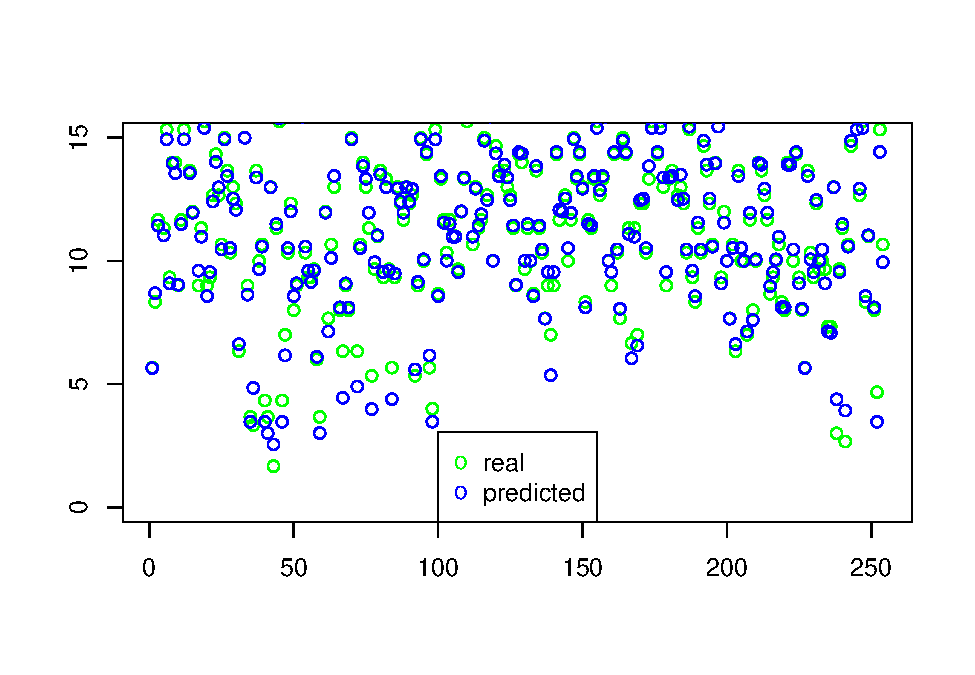
\includegraphics{Practica2_files/figure-latex/unnamed-chunk-52-1.pdf}

\begin{verbatim}
##   xchar= 7.792 ; (yextra, ychar)= 0, 1.218 
##   rect2(99.96,3.054, w=55.09, h=3.654, ...)
##   points2( 107.7 107.7 , 1.836 0.618 , pch= o o , ...)
\end{verbatim}

\hypertarget{regresion-logistica}{%
\subsection{Regresión logística}\label{regresion-logistica}}

Vamos a utilizar regresión logística para intentar averiguar qué
variable de las categóricas con las que hemos estado trabajando puede
predecirse mejor a partir de la nota media dle curso. Vamos a generar
modelos de regresión logística para distintas variables dicotómicas, y
vamos a ver cuál de ellos es mejor.

Nos centraremos en las siguientes variables:

\begin{itemize}
\tightlist
\item
  Sexo: podemos predecir el sexo del alumno en función de la nota?
\item
  SchoolSup: podemos predecir si el alumno ha tenido ayuda en la escuela
  en función de la nota media?
\item
  famSup: podemos predecir si el alumno ha tenido ayuda en casa en
  función de la nota media?
\item
  higher: Podemos predecir si el alumno querrá seguir estudiando en
  función de la nota media obtenida?
\end{itemize}

En primer lugar vamos a representar las observaciones para cada uno de
estos casos para poder intuir gráficamente si la varibale escogida (la
media de las notas: score) está relacionada con la variable respuesta
(obtienen ayuda escolar) y puede considerarse que es un buen predictor

\begin{Shaded}
\begin{Highlighting}[]
\KeywordTok{par}\NormalTok{(}\DataTypeTok{mfrow=}\KeywordTok{c}\NormalTok{(}\DecValTok{2}\NormalTok{,}\DecValTok{2}\NormalTok{))}
\KeywordTok{ggplot}\NormalTok{(}\DataTypeTok{data =}\NormalTok{ students, }\KeywordTok{aes}\NormalTok{(}\DataTypeTok{x =}\NormalTok{ sex, }\DataTypeTok{y =}\NormalTok{ score, }\DataTypeTok{color =}\NormalTok{ sex)) }\OperatorTok{+}
\StringTok{  }\KeywordTok{geom_boxplot}\NormalTok{(}\DataTypeTok{outlier.shape =} \OtherTok{NA}\NormalTok{) }\OperatorTok{+}
\StringTok{  }\KeywordTok{geom_jitter}\NormalTok{(}\DataTypeTok{width =} \FloatTok{0.1}\NormalTok{) }\OperatorTok{+}
\StringTok{  }\KeywordTok{theme_bw}\NormalTok{() }\OperatorTok{+}
\StringTok{  }\KeywordTok{theme}\NormalTok{(}\DataTypeTok{legend.position =} \StringTok{"null"}\NormalTok{)}
\end{Highlighting}
\end{Shaded}

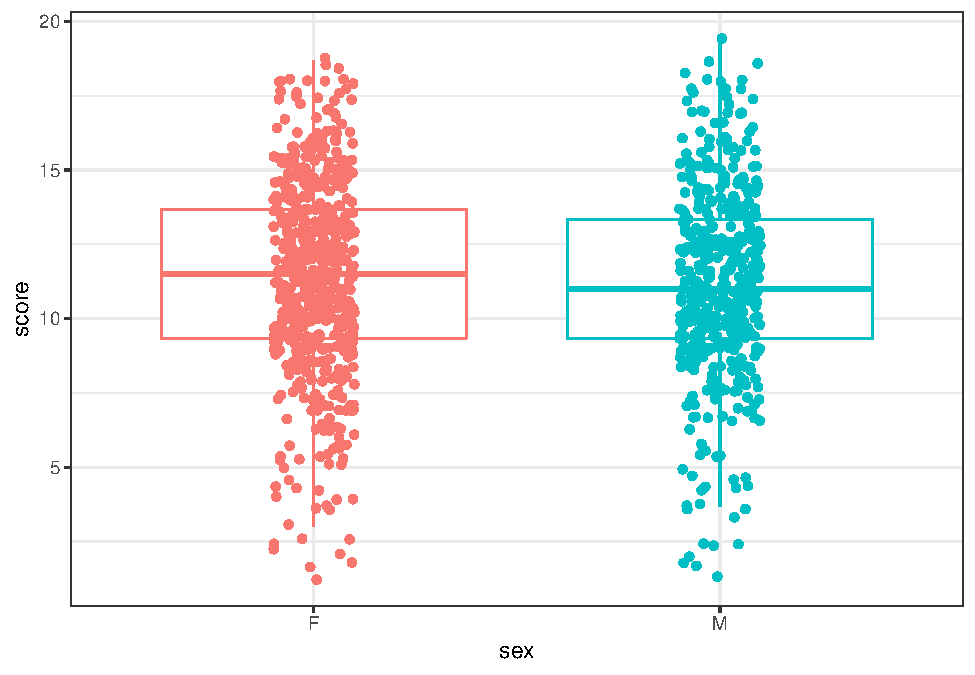
\includegraphics{Practica2_files/figure-latex/unnamed-chunk-53-1.pdf}

\begin{Shaded}
\begin{Highlighting}[]
\KeywordTok{ggplot}\NormalTok{(}\DataTypeTok{data =}\NormalTok{ students, }\KeywordTok{aes}\NormalTok{(}\DataTypeTok{x =}\NormalTok{ schoolsup, }\DataTypeTok{y =}\NormalTok{ score, }\DataTypeTok{color =}\NormalTok{ schoolsup)) }\OperatorTok{+}
\StringTok{  }\KeywordTok{geom_boxplot}\NormalTok{(}\DataTypeTok{outlier.shape =} \OtherTok{NA}\NormalTok{) }\OperatorTok{+}
\StringTok{  }\KeywordTok{geom_jitter}\NormalTok{(}\DataTypeTok{width =} \FloatTok{0.1}\NormalTok{) }\OperatorTok{+}
\StringTok{  }\KeywordTok{theme_bw}\NormalTok{() }\OperatorTok{+}
\StringTok{  }\KeywordTok{theme}\NormalTok{(}\DataTypeTok{legend.position =} \StringTok{"null"}\NormalTok{)}
\end{Highlighting}
\end{Shaded}

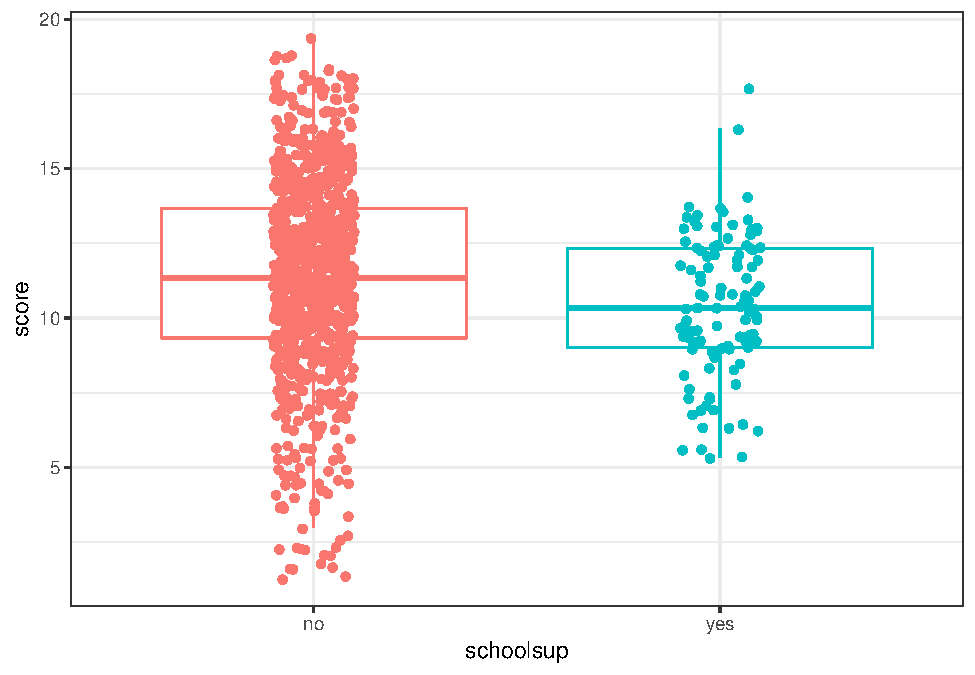
\includegraphics{Practica2_files/figure-latex/unnamed-chunk-53-2.pdf}

\begin{Shaded}
\begin{Highlighting}[]
\KeywordTok{ggplot}\NormalTok{(}\DataTypeTok{data =}\NormalTok{ students, }\KeywordTok{aes}\NormalTok{(}\DataTypeTok{x =}\NormalTok{ famsup, }\DataTypeTok{y =}\NormalTok{ score, }\DataTypeTok{color =}\NormalTok{ famsup)) }\OperatorTok{+}
\StringTok{  }\KeywordTok{geom_boxplot}\NormalTok{(}\DataTypeTok{outlier.shape =} \OtherTok{NA}\NormalTok{) }\OperatorTok{+}
\StringTok{  }\KeywordTok{geom_jitter}\NormalTok{(}\DataTypeTok{width =} \FloatTok{0.1}\NormalTok{) }\OperatorTok{+}
\StringTok{  }\KeywordTok{theme_bw}\NormalTok{() }\OperatorTok{+}
\StringTok{  }\KeywordTok{theme}\NormalTok{(}\DataTypeTok{legend.position =} \StringTok{"null"}\NormalTok{)}
\end{Highlighting}
\end{Shaded}

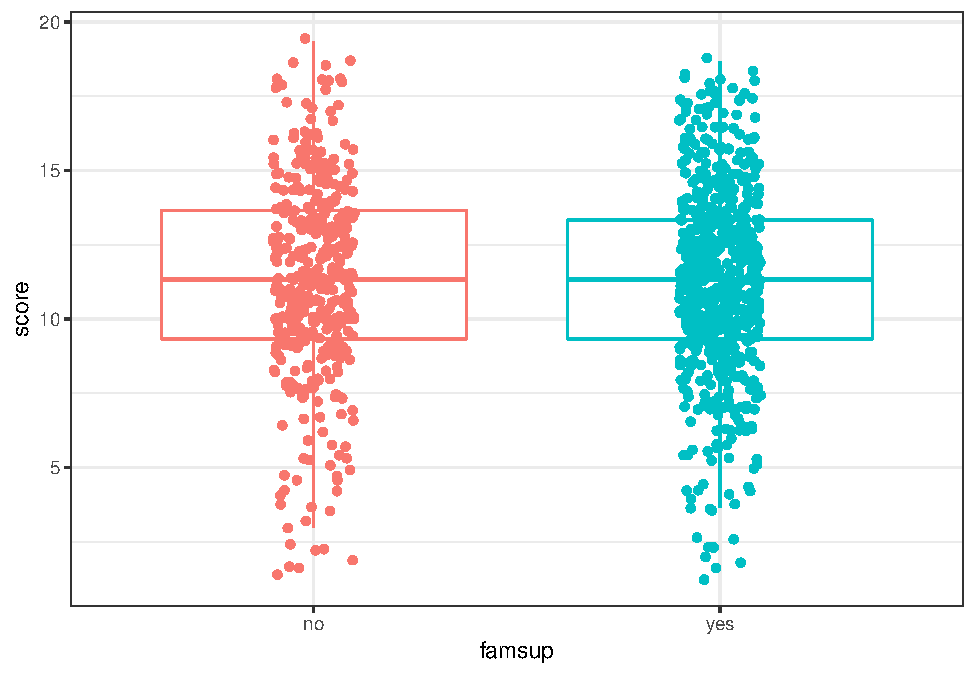
\includegraphics{Practica2_files/figure-latex/unnamed-chunk-53-3.pdf}

\begin{Shaded}
\begin{Highlighting}[]
\KeywordTok{ggplot}\NormalTok{(}\DataTypeTok{data =}\NormalTok{ students, }\KeywordTok{aes}\NormalTok{(}\DataTypeTok{x =}\NormalTok{ higher, }\DataTypeTok{y =}\NormalTok{ score, }\DataTypeTok{color =}\NormalTok{ higher)) }\OperatorTok{+}
\StringTok{  }\KeywordTok{geom_boxplot}\NormalTok{(}\DataTypeTok{outlier.shape =} \OtherTok{NA}\NormalTok{) }\OperatorTok{+}
\StringTok{  }\KeywordTok{geom_jitter}\NormalTok{(}\DataTypeTok{width =} \FloatTok{0.1}\NormalTok{) }\OperatorTok{+}
\StringTok{  }\KeywordTok{theme_bw}\NormalTok{() }\OperatorTok{+}
\StringTok{  }\KeywordTok{theme}\NormalTok{(}\DataTypeTok{legend.position =} \StringTok{"null"}\NormalTok{)}
\end{Highlighting}
\end{Shaded}

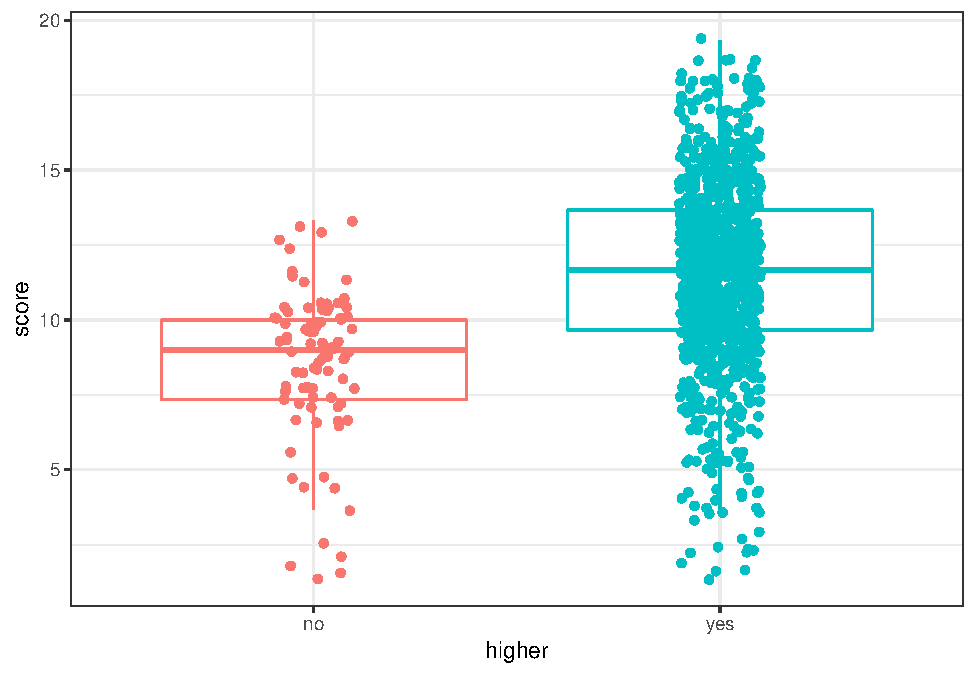
\includegraphics{Practica2_files/figure-latex/unnamed-chunk-53-4.pdf}

A la vista de las gráficas, parece que en el único caso en el que se
aprecian diferencias significativas en las notas es en el caso en el que
los estudiantes quieren seguir estudiando.

Ahora vamos a generar los modelos para cada una de ellas a ver qué
obtenemos

\begin{Shaded}
\begin{Highlighting}[]
\NormalTok{m1 <-}\StringTok{ }\KeywordTok{glm}\NormalTok{(sex }\OperatorTok{~}\StringTok{ }\NormalTok{score, }\DataTypeTok{data =}\NormalTok{ students, }\DataTypeTok{family =} \StringTok{"binomial"}\NormalTok{)}
\KeywordTok{summary}\NormalTok{(m1)}
\end{Highlighting}
\end{Shaded}

\begin{verbatim}
## 
## Call:
## glm(formula = sex ~ score, family = "binomial", data = students)
## 
## Deviance Residuals: 
##    Min      1Q  Median      3Q     Max  
## -1.119  -1.064  -1.041   1.293   1.346  
## 
## Coefficients:
##             Estimate Std. Error z value Pr(>|z|)
## (Intercept) -0.12144    0.22984  -0.528    0.597
## score       -0.01380    0.01957  -0.705    0.481
## 
## (Dispersion parameter for binomial family taken to be 1)
## 
##     Null deviance: 1389.1  on 1015  degrees of freedom
## Residual deviance: 1388.6  on 1014  degrees of freedom
## AIC: 1392.6
## 
## Number of Fisher Scoring iterations: 4
\end{verbatim}

\begin{Shaded}
\begin{Highlighting}[]
\NormalTok{m2 <-}\StringTok{ }\KeywordTok{glm}\NormalTok{(schoolsup }\OperatorTok{~}\StringTok{ }\NormalTok{score, }\DataTypeTok{data =}\NormalTok{ students, }\DataTypeTok{family =} \StringTok{"binomial"}\NormalTok{)}
\KeywordTok{summary}\NormalTok{(m2)}
\end{Highlighting}
\end{Shaded}

\begin{verbatim}
## 
## Call:
## glm(formula = schoolsup ~ score, family = "binomial", data = students)
## 
## Deviance Residuals: 
##     Min       1Q   Median       3Q      Max  
## -0.7553  -0.5148  -0.4604  -0.4047   2.3777  
## 
## Coefficients:
##             Estimate Std. Error z value Pr(>|z|)    
## (Intercept) -0.97320    0.33213  -2.930 0.003388 ** 
## score       -0.10147    0.03021  -3.359 0.000783 ***
## ---
## Signif. codes:  0 '***' 0.001 '**' 0.01 '*' 0.05 '.' 0.1 ' ' 1
## 
## (Dispersion parameter for binomial family taken to be 1)
## 
##     Null deviance: 709.29  on 1015  degrees of freedom
## Residual deviance: 698.08  on 1014  degrees of freedom
## AIC: 702.08
## 
## Number of Fisher Scoring iterations: 5
\end{verbatim}

\begin{Shaded}
\begin{Highlighting}[]
\NormalTok{m3 <-}\StringTok{ }\KeywordTok{glm}\NormalTok{(famsup }\OperatorTok{~}\StringTok{ }\NormalTok{score, }\DataTypeTok{data =}\NormalTok{ students, }\DataTypeTok{family =} \StringTok{"binomial"}\NormalTok{)}
\KeywordTok{summary}\NormalTok{(m3)}
\end{Highlighting}
\end{Shaded}

\begin{verbatim}
## 
## Call:
## glm(formula = famsup ~ score, family = "binomial", data = students)
## 
## Deviance Residuals: 
##     Min       1Q   Median       3Q      Max  
## -1.3861  -1.3772   0.9872   0.9895   0.9941  
## 
## Coefficients:
##              Estimate Std. Error z value Pr(>|z|)  
## (Intercept)  0.480656   0.234243   2.052   0.0402 *
## score       -0.001761   0.019911  -0.088   0.9295  
## ---
## Signif. codes:  0 '***' 0.001 '**' 0.01 '*' 0.05 '.' 0.1 ' ' 1
## 
## (Dispersion parameter for binomial family taken to be 1)
## 
##     Null deviance: 1356.0  on 1015  degrees of freedom
## Residual deviance: 1355.9  on 1014  degrees of freedom
## AIC: 1359.9
## 
## Number of Fisher Scoring iterations: 4
\end{verbatim}

\begin{Shaded}
\begin{Highlighting}[]
\NormalTok{m4 <-}\StringTok{ }\KeywordTok{glm}\NormalTok{(higher }\OperatorTok{~}\StringTok{ }\NormalTok{score, }\DataTypeTok{data =}\NormalTok{ students, }\DataTypeTok{family =} \StringTok{"binomial"}\NormalTok{)}
\KeywordTok{summary}\NormalTok{(m4)}
\end{Highlighting}
\end{Shaded}

\begin{verbatim}
## 
## Call:
## glm(formula = higher ~ score, family = "binomial", data = students)
## 
## Deviance Residuals: 
##     Min       1Q   Median       3Q      Max  
## -2.5849   0.2226   0.3234   0.4261   1.2286  
## 
## Coefficients:
##             Estimate Std. Error z value Pr(>|z|)    
## (Intercept) -0.50010    0.34669  -1.443    0.149    
## score        0.28537    0.03613   7.898 2.84e-15 ***
## ---
## Signif. codes:  0 '***' 0.001 '**' 0.01 '*' 0.05 '.' 0.1 ' ' 1
## 
## (Dispersion parameter for binomial family taken to be 1)
## 
##     Null deviance: 589.22  on 1015  degrees of freedom
## Residual deviance: 521.16  on 1014  degrees of freedom
## AIC: 525.16
## 
## Number of Fisher Scoring iterations: 6
\end{verbatim}

Se observa que el AIC (criterio de información de Akaike) menor de los 4
modelos es el correspondiente al hecho de querer cursar estudios
superiores

\hypertarget{conclusiones}{%
\subsection{Conclusiones}\label{conclusiones}}

\hypertarget{recursos}{%
\section{Recursos}\label{recursos}}

Los siguientes recursos son de utilidad para la realización de la
práctica: ● Calvo M., Subirats L., Pérez D. (2019). Introducción a la
limpieza y análisis de los datos. Editorial UOC. ● Megan Squire (2015).
Clean Data. Packt Publishing Ltd. ● Jiawei Han, Micheine Kamber, Jian
Pei (2012). Data mining: concepts and techniques. Morgan Kaufmann. ●
Jason W. Osborne (2010). Data Cleaning Basics: Best Practices in Dealing
with Extreme Scores. Newborn and Infant Nursing Reviews; 10 (1):
pp.~1527-3369. ● Peter Dalgaard (2008). Introductory statistics with R.
Springer Science \& Business Media. ● Wes McKinney (2012). Python for
Data Analysis. O'Reilley Media, Inc. ● Tutorial de Github
\url{https://guides.github.com/activities/hello-world}.


\end{document}
